
\documentclass[preprint,12pt]{elsarticle}
\usepackage{amsmath,fullpage,graphicx,caption,float}
\usepackage{amssymb}
\usepackage{array,ragged2e,pst-node,pst-dbicons}
\usepackage{pstricks}
\usepackage{pst-node}
\usepackage{pst-blur}
\usepackage{comment}
\usepackage{color}
\usepackage{subfigure}
\usepackage{lscape}
\usepackage{multirow}
\usepackage{hyperref}
\usepackage{mathtools}
\usepackage{siunitx}
\newcommand{\defeq}{\vcentcolon=}


\usepackage{float}
\restylefloat{table}
\usepackage[margin=20mm]{geometry}

\setlength{\parskip}{1.25ex}
\renewcommand\baselinestretch{1.3}
\renewcommand\arraystretch{1.5}

% equation numbering:
\numberwithin{equation}{section}

\mathchardef\mhyphen="2D
\definecolor{Pink}{rgb}{1.,0.75,0.8}
\newcolumntype{C}[1]{>{\Centering}p{#1}}
\def\Tab#1{\tabular{C{3cm}}\rule[-5mm]{0pt}{1cm}#1\\\hline
                           ~\\\hline~\endtabular}
\seticonparams{entity}{shadow,fillcolor=black!20,fillstyle=solid,framesep=0pt}

\mathchardef\mhyphen="2D


\journal{Nuclear Instruments and Methods}

\begin{document}

\begin{frontmatter}



\title{Time Of Flight System for CLAS12}

%% use optional labels to link authors explicitly to addresses:
\author[USC]{R.~W.~Gothe}
\author[USC]{G.~V.~Fedotov}
\author[USC]{E.~Phelps}
\author[USC]{Iu.~Skorodumina}
\author[USC]{Y.~Tian}
\author[USC]{A.~Trivedi}
\author[USC]{N.~Tyler}

\address[USC]{University of South Carolina, Columbia, South Carolina 29208}
%% \address[label2]{<address>}

\author{}

\address{}

\begin{abstract}
In this paper the process of developing and testing of TOF system for CLAS12 is described. To speed up testing process new so-called ``6-bar'' method of time resolution determination using cosmic rays is developed. With new measuring procedure the world record time resolution for given scintilliator length is achived.  

\end{abstract}

\begin{keyword}
TOF, Nuclear physics experiment
%% keywords here, in the form: keyword \sep keyword

%% MSC codes here, in the form: \MSC code \sep code
%% or \MSC[2008] code \sep code (2000 is the default)

\end{keyword}

\end{frontmatter}


\pagebreak





\section{12-GeV upgrade and CLAS12 overview}
\label{12GeV}

%\subsection{Detector-based rather than physics-based}
%\subsection{Condense content of other CLAS12 publications}
%\subsection{Highlight significance of each detector subsystem for particle reconstruction in different kinematic regimes}

{\it Note:\\
Detector-based rather than physics-based.\\
Condense content of other CLAS12 publications.\\
Highlight specific requirement of each detector subsystem for particle reconstruction in different kinematic regimes.\\
Segue into next section FTOF12 \\

Important figures: \\
complete detector $\rightarrow$ FTOF12 at that level
}

\begin{figure}[h!]
\centering
\mbox{\subfigure[$\:$FTOF panels installed in Hall-B.]{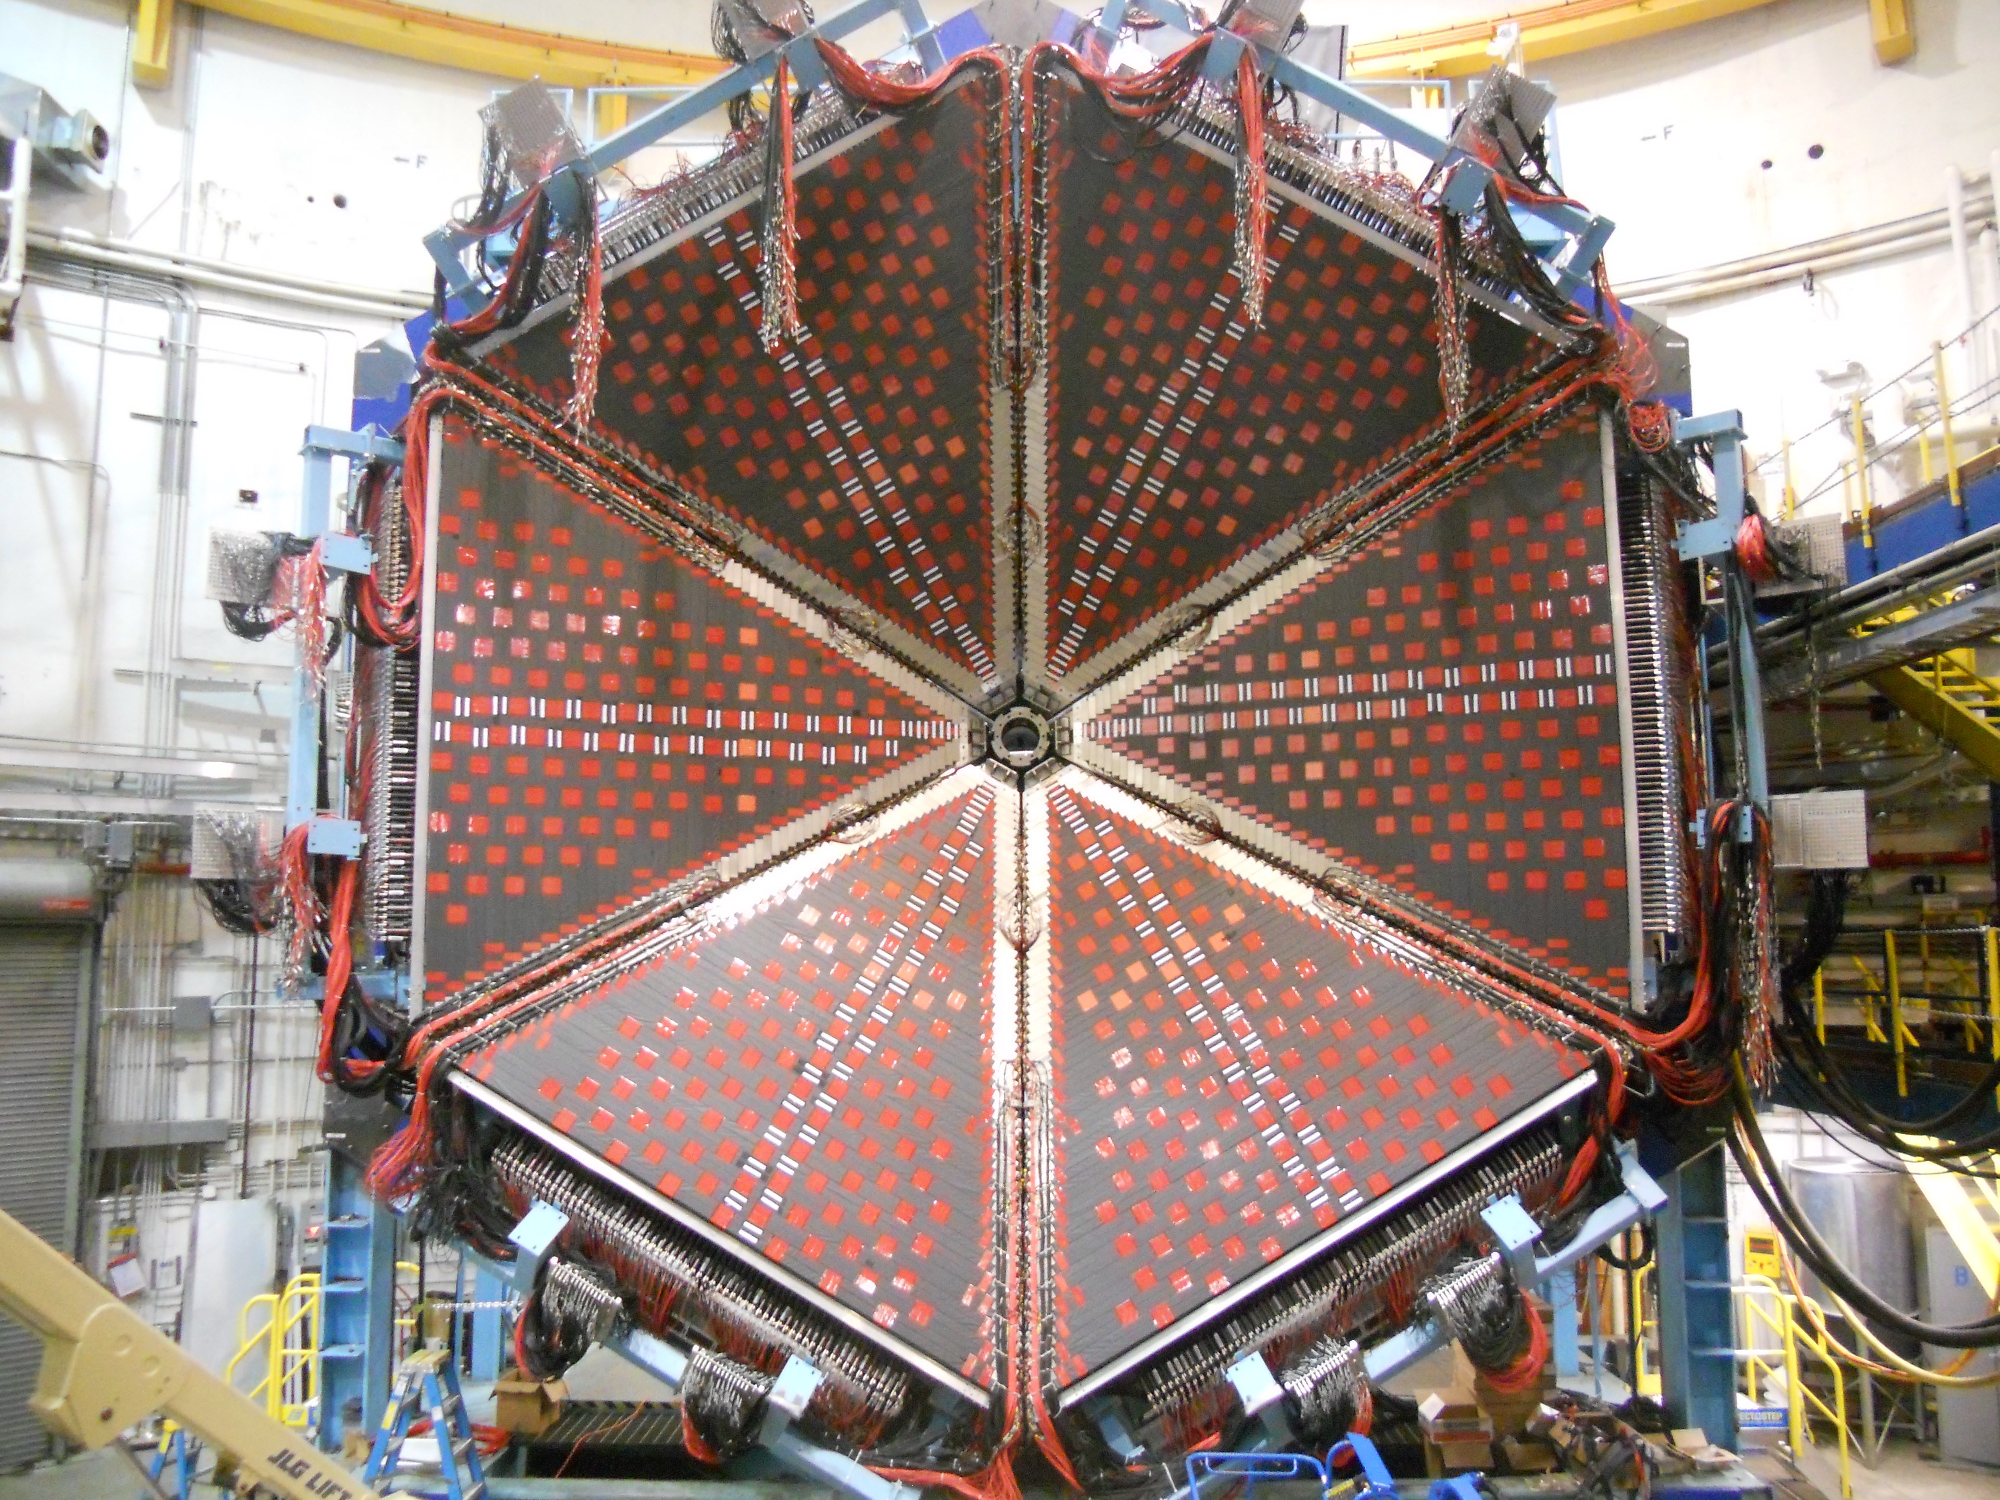
\includegraphics[width=0.4\textwidth]{ralf/fig_ralf_12gev_upgrade/tof_installed1.pdf}}\quad
\subfigure[$\:$FTOF installation process.]{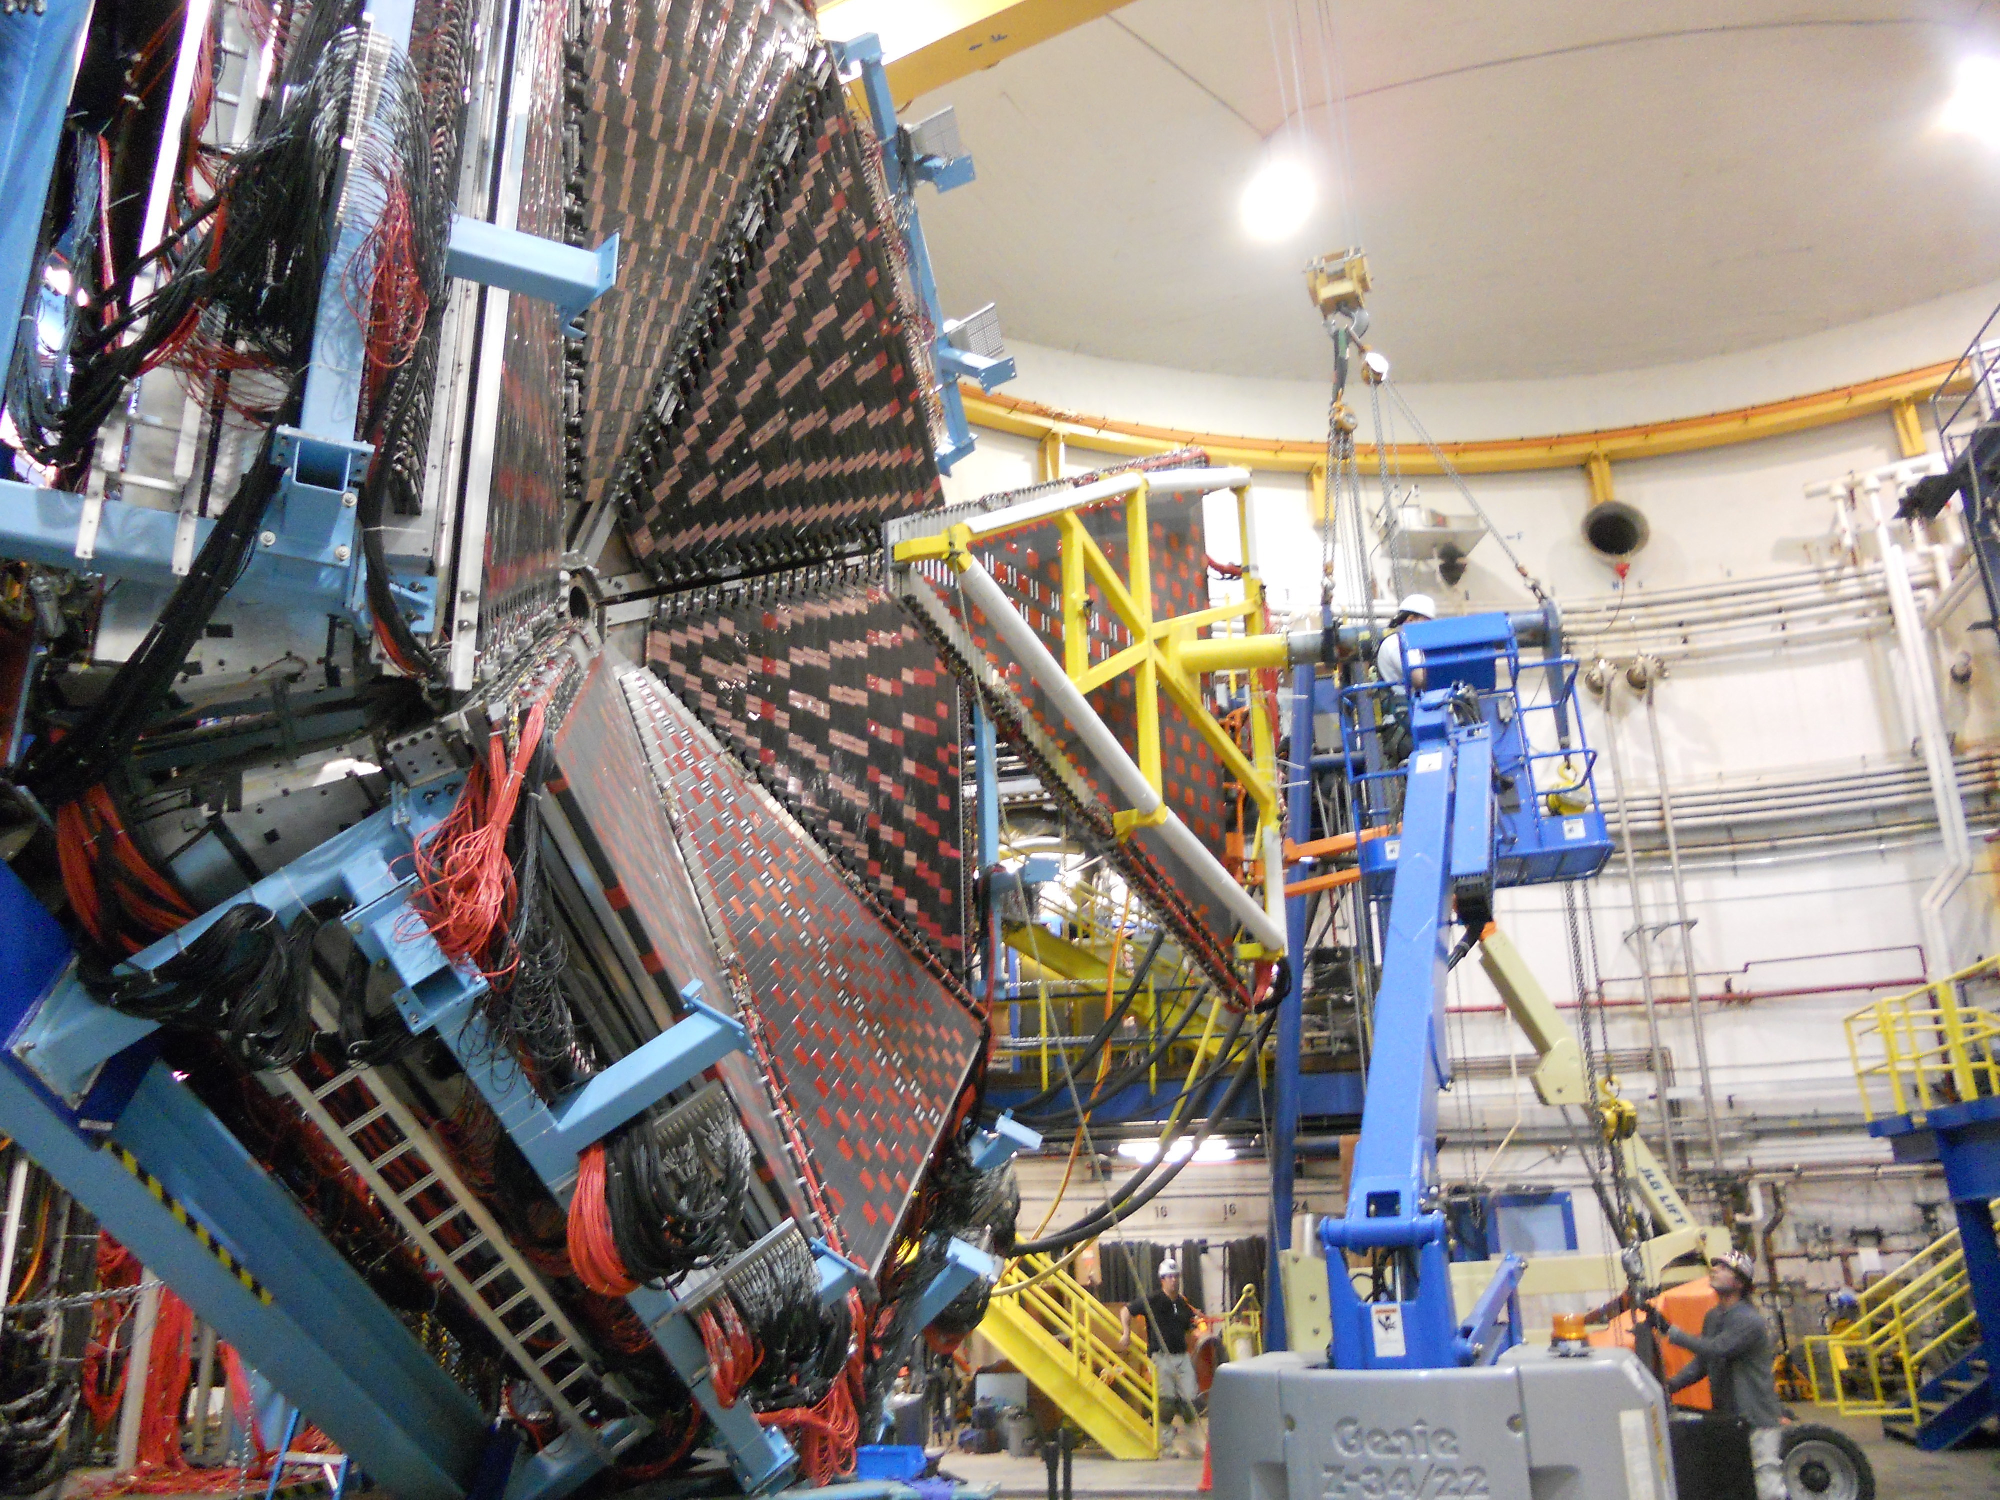
\includegraphics[width=0.4\textwidth]{ralf/fig_ralf_12gev_upgrade/tof_installed2.pdf}}}
\caption{\label{fig:tof_installed}\label{fig:tof_installation}}
\end{figure}

\section{FTOF12 requirements and high-level design}
\label{FTOF12}


{\it Important figures:\\
particle separation curves on t vs. p assuming 4separation (p$K$, $K\pi$, p$\pi$).  print quality version of some combination of these: \\
resolution curves on time resolution vs. counter length (old, new, combined) \\
resolution curves on time resolution vs. counter length per scintillator material (per advertised attenuation lengths)\\
CLAS12 geometry $\rightarrow$ FTOF12 geometry (zoom in, light guides and PMT form-factors)
stray B-field map (or just state upper bound)\\
stray B-field map (or just state upper bound)
}

The time-of-flight subsystem of the CLAS detector in Hall B was designed to allow separation of pions and kaons in the kinematic range accessible with a $6$-$GeV$ electron beam by providing time resolutions from $90\:ps$ to $160\:ps$ at the forward angles, where the most energetic particles are detected.~\cite{clastof} To reliably separate $p$, $\pi$, and $K$ in the kinematic range accessible with the proposed $11$-$GeV$ beam of the CEBAF upgrade, the FTOF detector must achieve a resolution of $80\:ps$~\cite{tdr} as illustrated in Fig.$\:$\ref{fig:partIdReq}. This assumes a $4\sigma$ time difference between two particles, thus allowing for identification of a signal in the presence of other particles with a ten-fold higher rate.
\begin{figure}[h!]
\centerline{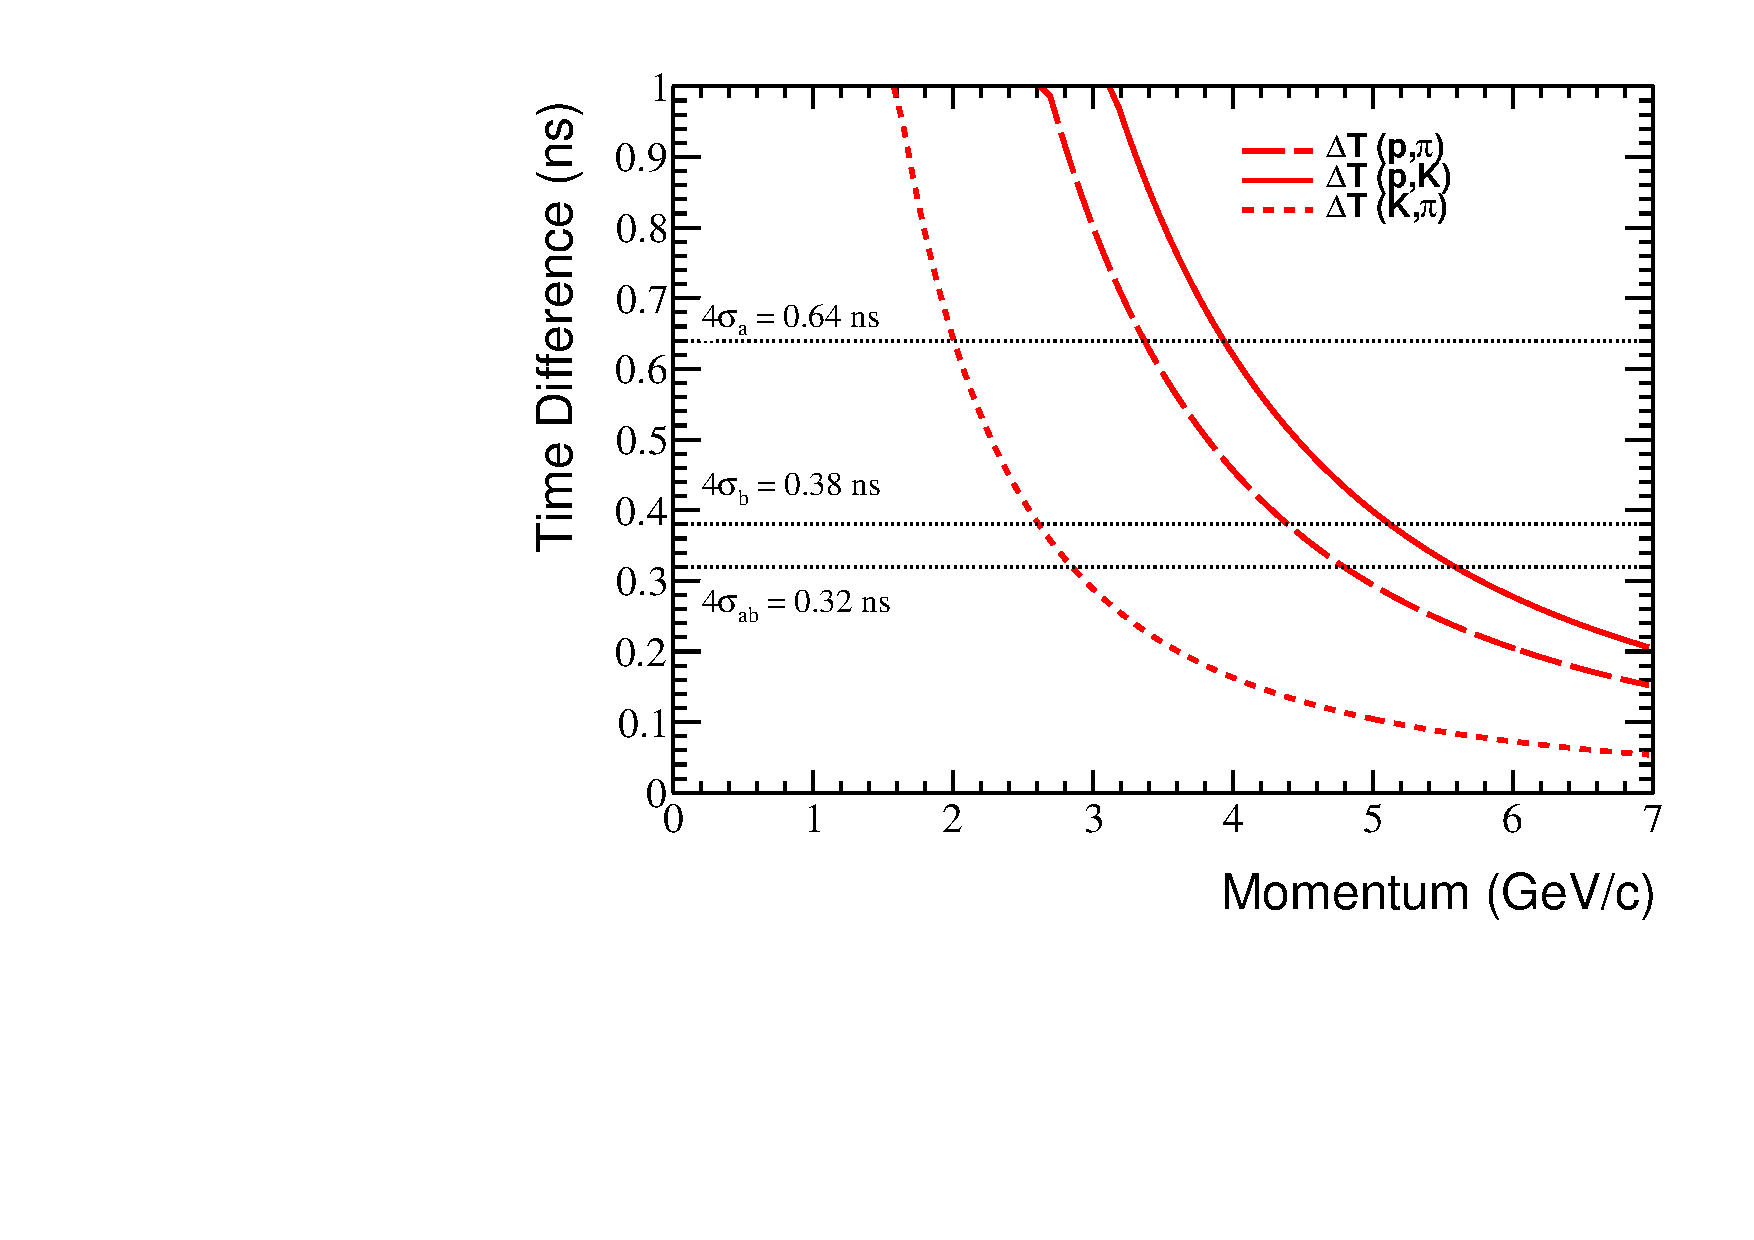
\includegraphics[width=6cm,height=6cm]{evan/fig_evan_ftof_requirements/DeltaT.pdf}}
\caption{The three curves indicate the time differences,$\Delta t$, between $p/\pi$,$p/K$, and $\pi/K$ over the $650\;cm$ path length from the target to Panel 1B. }
\label{fig:DeltaT}
\end{figure}
\begin{figure}[h!]
\centering
\mbox{\subfigure[$\:$Particle separation.]{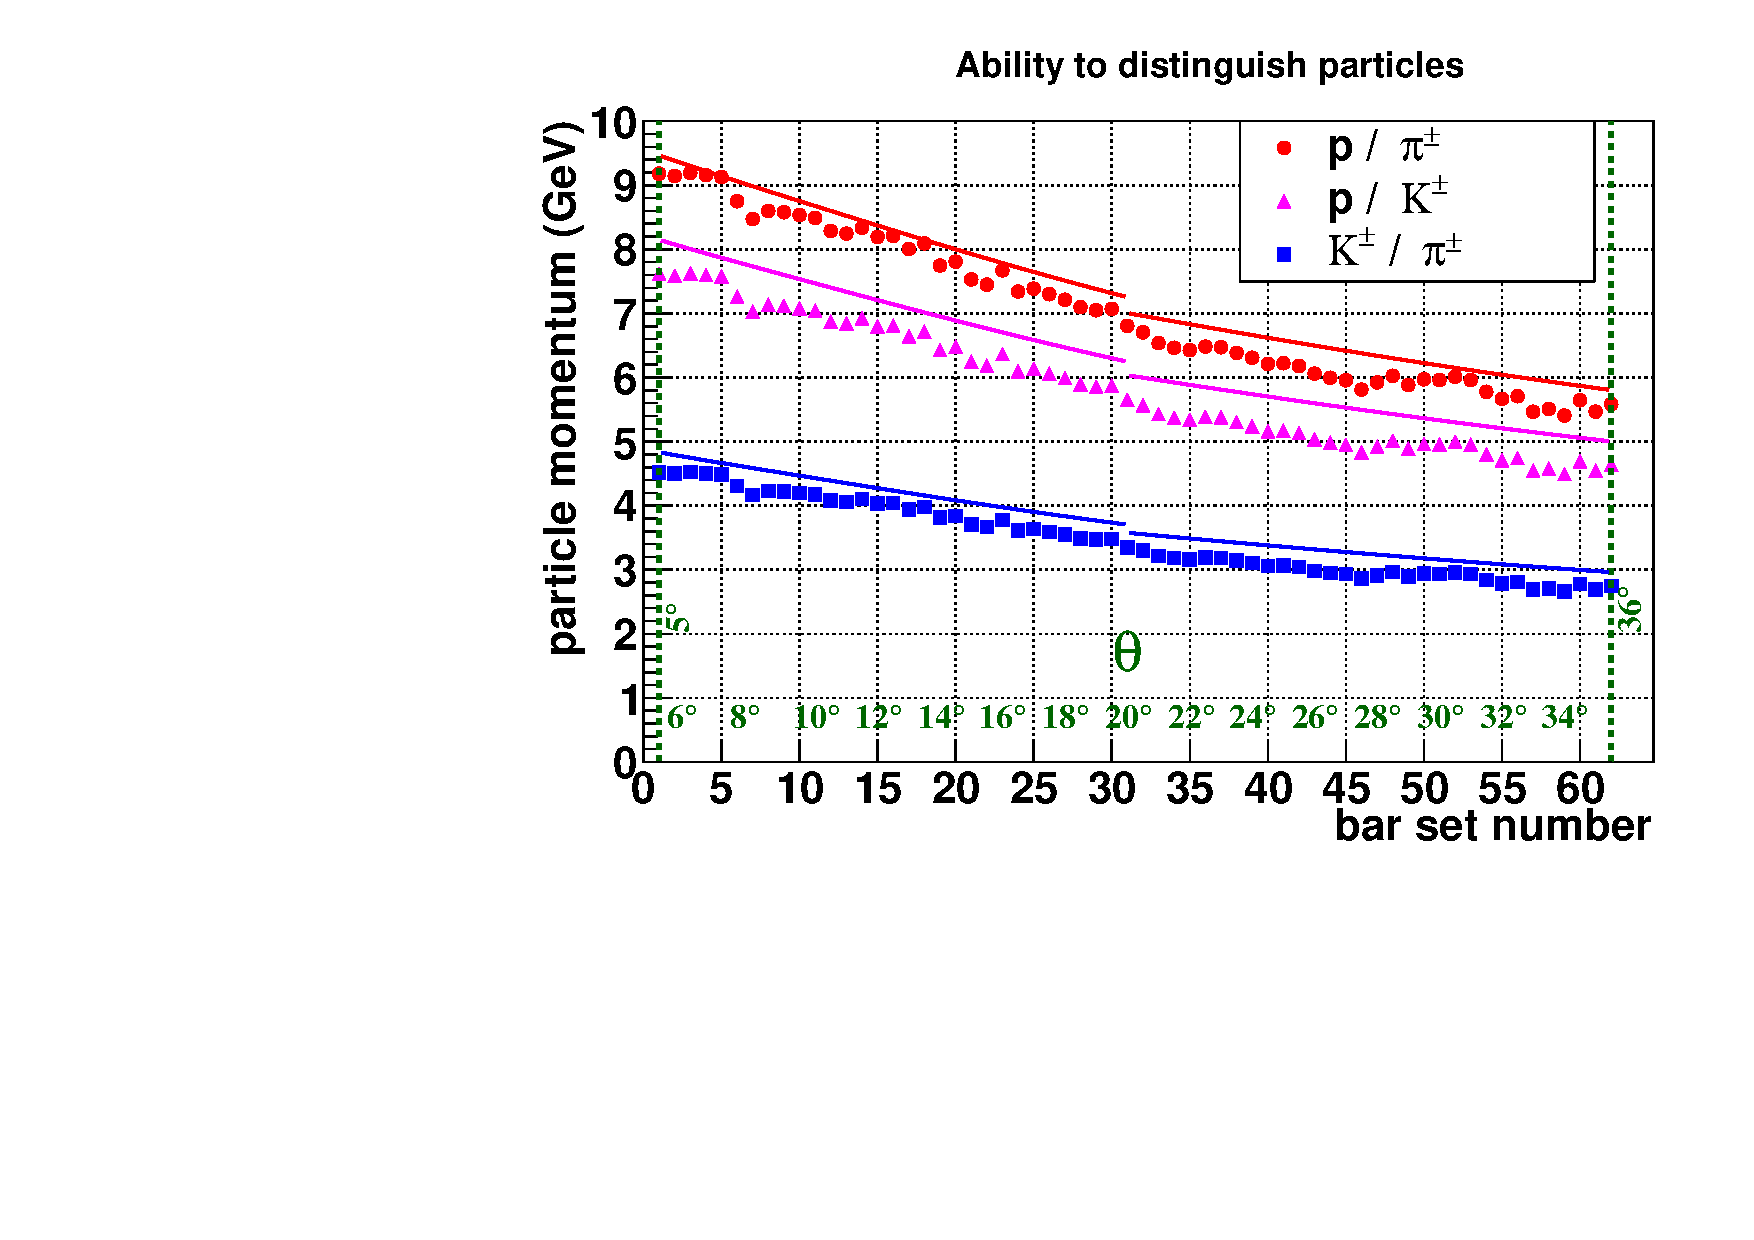
\includegraphics[width=0.4\textwidth]{evan/fig_evan_ftof_requirements/p_max.pdf}}\quad
\subfigure[$\:$Resolution curves.]{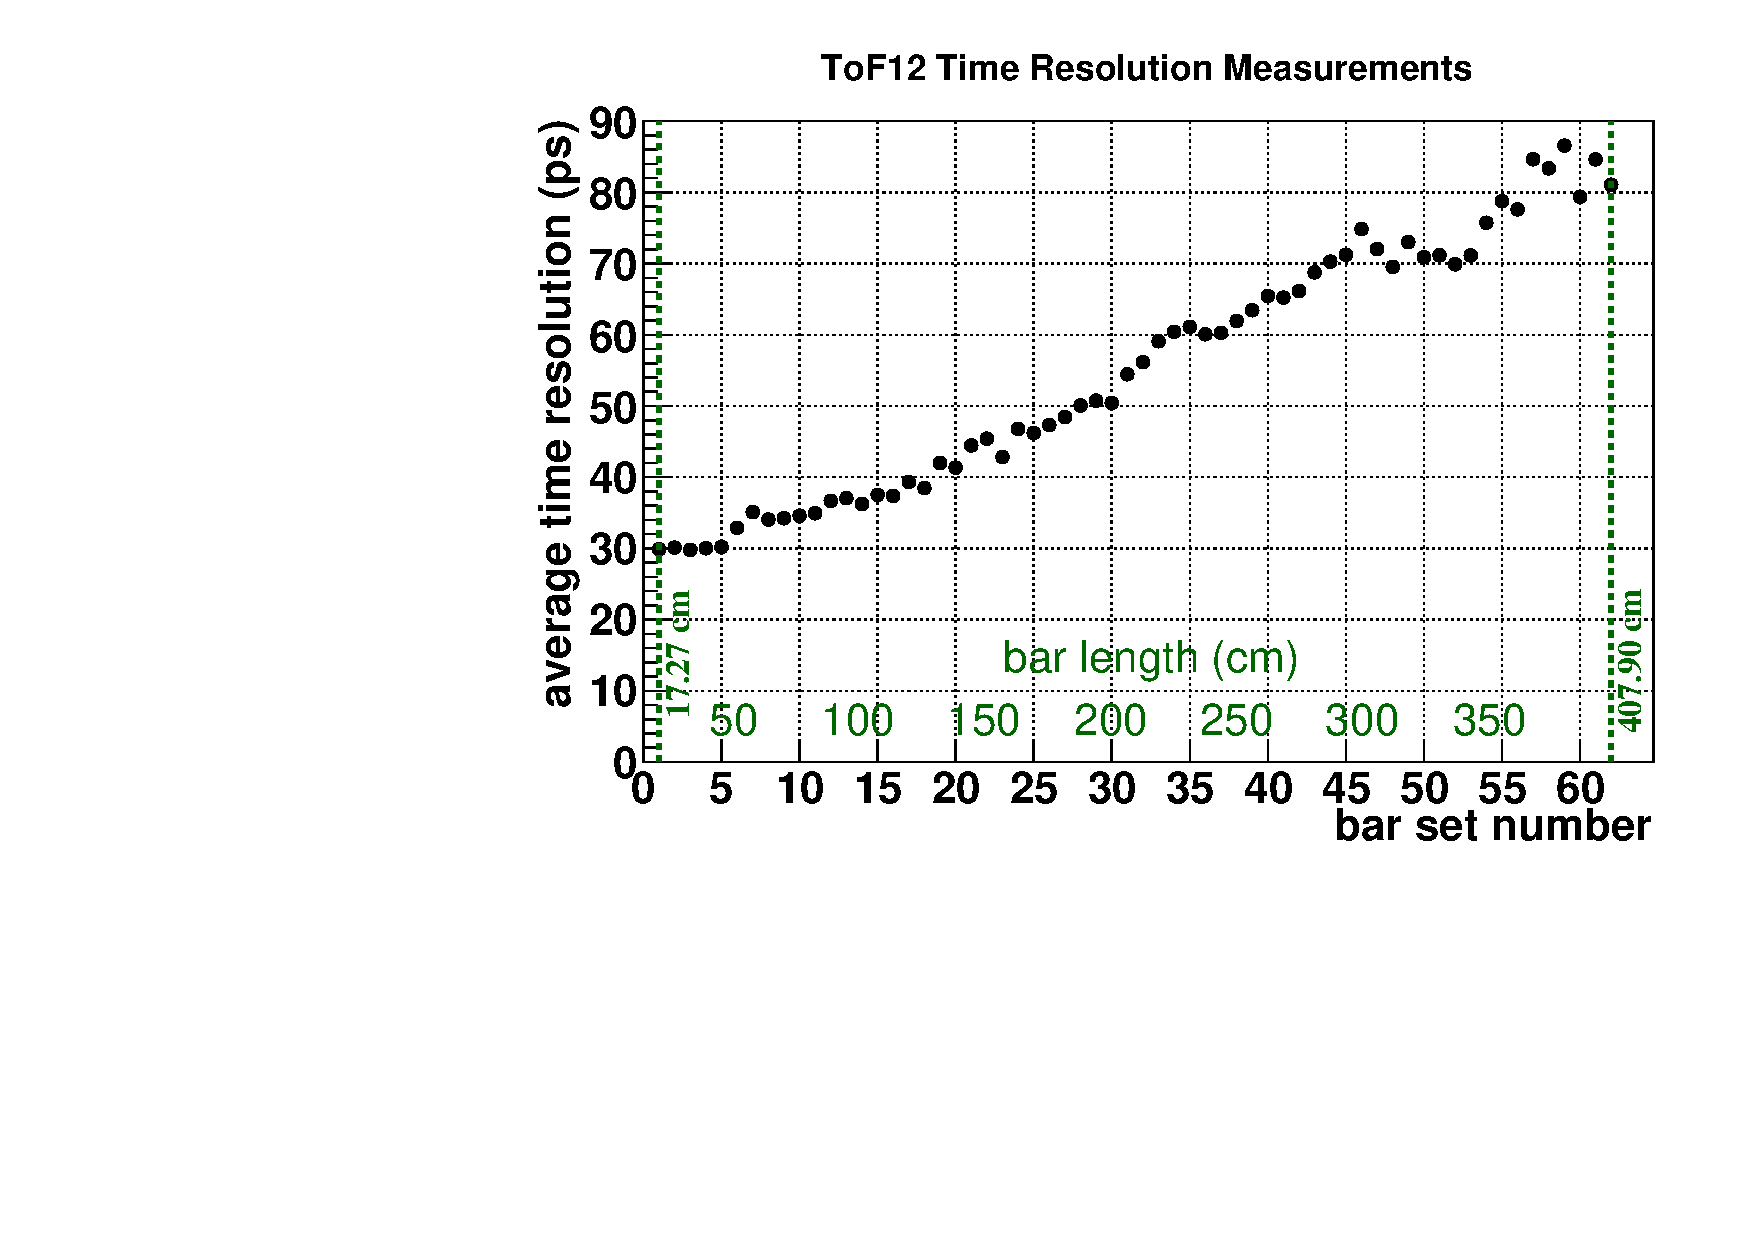
\includegraphics[width=0.4\textwidth]{evan/fig_evan_ftof_requirements/res.pdf}}}
\caption{(a) Maximum momentum up to which particles can be separated as function of bar set number or polar angle thete. Calculations were made in assumption of 650-$cm$ path length from the target to Panel 1B.~\cite{tdr}. Various symbols represent different particle pairs:  red circles - $p$/$\pi$, purple triangles - $p$/$K$, and  blue squares - $K$/$/pi$. (b) Average time resolution as function of bar set number or bar length. Black circles represent measurements performed at USC, while blue squares correspond to JLab measurements. For USC results resolutions of individual bars were averaged, while for JLab results resolution of three bar combinations were averaged. \label{fig:partIdReq}\label{fig:resLength}}
\end{figure}

As in the current $6$-$GeV$ FTOF detector (Panel 1A), each counter of the additional $12$-$GeV$ FTOF (Panel 1B) is composed of a long rectangular plastic scintillator with two cylindrical PMTs, one on each end, directly attached without light guides. The scintillator lengths are tightly constrained by the established six-panel FTOF geometry and the requirement that the new panels do not  restrict the CLAS12 acceptance as defined by the other detector components, but the thickness and width, $6\:cm \times 6\:cm$, are selected to optimize photon statistics, geometric matching with the photocathodes, and closest possible stacking. Compared to the Panel-1A $5\:cm \times 15\:cm$ FTOF scintillators, the $6\:cm \times 6\:cm$ scintillators increase the number of photons produced by a factor of 6/5; the increased ratio of photocathode area to scintillator exit window area increases the number of photons that reach the photocathode by at least a factor of 25/12.  Thus, disregarding that the area ratio factor acts on the number of photons after light attenuation, the Panel-1B scintillator geometry increases the number of photons reaching the photocathode by a factor of about 5/2 and, therefore, improves the resolution by a factor of $\sqrt{2/5}$, neglecting the resolution of any contributions that are independent of light level.

With a resolution of better than $150\:ps$ for the longest counters of Panel 1A, the Panel-1B counters must achieve resolutions better than $95\:ps$ for the combined resolution goal of $80\:ps$ to be reached (Fig.$\:$\ref{fig:resLength}). Preliminary prototype results exceed this requirement.

\subsubsection{Source method}
\label{sect:Source_method}

One of the methods that can be used to determine counter resolution is so called "source" or "coordinate method" (see CLAS-NOTE 2004-016 \cite{knu-clasnote}) that is based on the fact that the light flash coordinate and arrival times of signals in two PMTs are correlated. In this method radioactive small Sr-90 $\beta$-source is placed in various positions along the bar in order to measure position-specific resolution. 

For given project this method is highly inappropriate for two main reasons: (a) large number of counters (372) with length up to four meters leads to huge amount of manual measurements; (b) the Sr-90 events
are not representative neither in penetration depth nor photon statistics, since energy of $\beta$-particles from the source is in order of MeV, while particles that will be measured in CLAS12 have energy order of GeV.

Thus this method was used for initial electronic and selected individual counters test only.

\subsubsection{Thin scintillator cosmic ray method}
\label{sect:Thin_scintillator}

Another method of counter resolution determination is so-called "thin scintillator cosmic rays method" that uses two thin scintillators to effectively collimate cosmic rays
trajectories to perpendicularly traverse the counter at a fixed position, as shown in Fig.$\:$\ref{fig:thin_method1}. In this method time information from top and bottom counters is not needed. In order to fix track position signal coincidence  in six PMTs is required. This method was tested using five millimeters thin scintillators and it turned out that event rate is extremely low. Moreover, like in source method described in Sec.~\ref{sect:Source_method} huge amount of manual measurements is needed. 

\begin{figure}[]
\centering
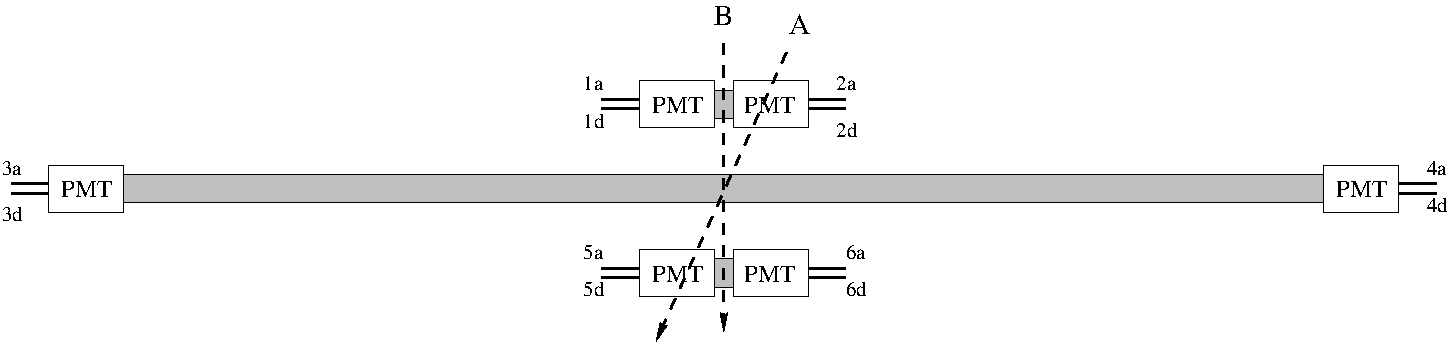
\includegraphics[width=0.9\textwidth]{gleb/fig_gleb_thin_scintillator/thin_method1.pdf}
\caption{In the thin scintillator cosmic ray  method, 5mm-thin scintillators are placed above and below the
counter to be tested so that the position of cosmic ray events on the middle counter is fixed. The
TDC difference between left and right PMTs on the middle counter is then used to determine the
counter's resolution. Only vertical tracks such as B survive, when signals in six PMTs are in coincidence. \label{fig:thin_method1}}
\end{figure}

In order to increase event rate this method can be modified as shown in Fig.$\:$\ref{fig:thin_method2}. In that case one thin scintillator ten times thicker than in previous setup is positioned between two longer scintillators achieving a partial collimation. Since non vertical tracks shown as A on Fig.$\:$\ref{fig:thin_method2} pass only part of the middle scintillator height, amplitudes of their signals are lower  then from the vertical tracks shown by B on Fig.$\:$\ref{fig:thin_method2}. So the positions on top and bottom scintillators are further restricted by cutting away low ADC events on the middle bar. But it turned out that this procedure does not sufficiently increase event rate and does not allow to get rid of the multiple manual measurements.




\begin{figure}[]
\centering
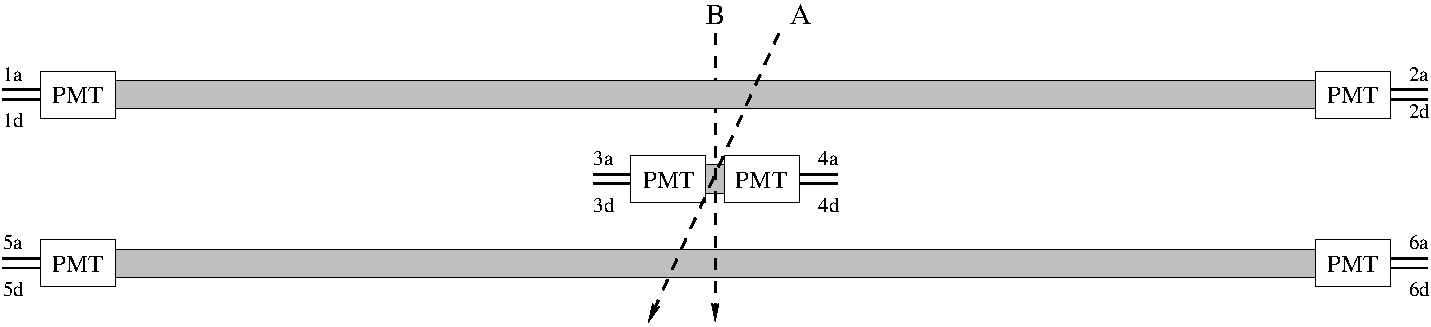
\includegraphics[width=0.9\textwidth]{gleb/fig_gleb_thin_scintillator/thin_method2.pdf}
\caption{This variant of the reference counter method does not physically restrict particles to pass
through vertically (path B), because particles along path A also triggers all six PMTs. However,
paths such as A are further reduced by cutting away middle-bar low ADC values, which correspond
generally to particles traveling through less than the 5-cm vertical extent of the middle scintillator.\label{fig:thin_method2}}
\end{figure}


Both described variants of thin scintillator cosmic rays method can be transformed into so-called "reference counter method", in which thin scintillator counters need to be replaced by reference counters with known resolutions. In that case one should use TDC information from reference counters and vertical tracks selection is not needed anymore that lead to the higher event rate. Then it becomes possible for setup like shown on Fig.$\:$\ref{fig:thin_method1} to derive the resolution of tested counter through the resulutions of reference counters, and for setup like shown on Fig.$\:$\ref{fig:thin_method2}  to derive the combined resolution of two tested counters through the resolution of the known one. 

In case of the need to test many similar counters it is natural to build setup from the three counters of the same lenght and to extract their combined resolution. These modifications lead to the three bar cosmic rays method described in Sec.~\ref{sect:Three_Bar_Cosmic_Ray_Method}

\section{Six Bar Cosmic-Ray Method}

The six bar cosmic-ray method is a generalization and improvement of
the three bar cosmic-ray method facilitating individual counter
resolution measurements.  As such, it is necessary to recapitulate the
three bar cosmic-ray method prior to presenting the six bar cosmic-ray
method.

\subsection{Three Bar Cosmic-Ray Method}
\label{sect:Three_Bar_Cosmic_Ray_Method}

The three bar cosmic-ray method (hereafter known as the three bar
method) allows the determination of the time resolution of a counter
given two counters with known time resolutions.  A counter here is a
scintillator with photomultiplier tubes (PMTs) attached at each end.
The three bar cosmic-ray method proceeds by stacking the three
counters vertically with equal spacing between adjacent counters and
each counter being parallel to the other two.

\begin{figure}[H]
  \centering
  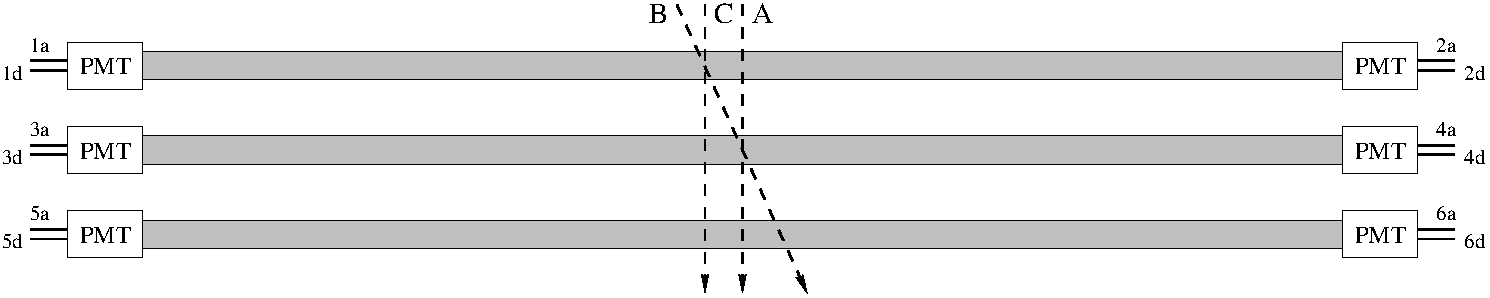
\includegraphics[width=15cm]{gary/fig_gary_three_bar/Fig14-M.pdf}
  \caption{In the three bar method, cosmic-ray particles are required
    to pass through all three counters.  A, B, and C denote possible
    particle paths through the three counters.}
  \label{3bar}
\end{figure}

%% This figure was deprecated due to earlier (and better) figure for
%% the three bar setup

%% \begin{figure}[H]
%%   \centering
%%   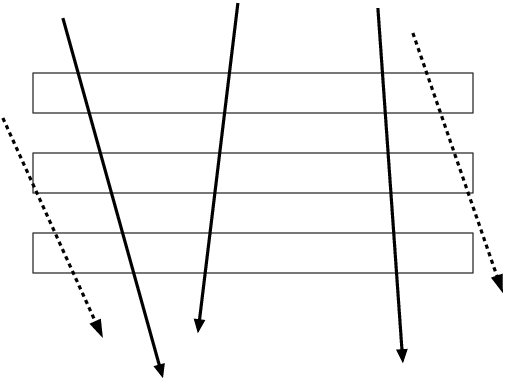
\includegraphics[width=15cm]{3bar.png}
%%   \caption{In the three bar method, cosmic-ray particles are required
%%     to pass through all three counters; solid lines illustrate
%%     detected particle tracks whereas dashed lines show discarded
%%     paths.}
%%   \label{3bar}
%% \end{figure}

Cosmic-ray particles will interact with the counters at random.  If
only those events in which all three counters detected a cosmic-ray
particle are considered, then the geometry of the setup allows the
unknown resolution to be determined.  The detected cosmic-ray
particles are assumed to have high enough energy so that the paths
they take are straight to good approximation (a good assumption in
practice).  Since the counters are arranged to be parallel with equal
spacing, and since the particle travels with fixed velocity, the time
taken to travel between any pair of adjacent counters is the same.

The interacting cosmic-ray particle causes each PMT to signal; these
are sent to a time-to-digital converter (TDC) and reported as the
interaction time of the scintillation light with the PMT.  One of the
six PMTs is chosen to provide the reference time for the event
\(t_{ref}\).  The reference time is subtracted from the raw time
reported from the TDC for each PMT since the raw TDC reported times
have arbitrary offsets.  Therefore the reference-subtracted timing for
each PMT is given by \(t = t_{\mathrm{raw}} - t_{ref}\).

The time that the cosmic-ray particle interacts with the
\(i\mathrm{th}\) scintillator is given by

\begin{equation}
  t'_i = \frac{t_{iL} + t_{iR}}{2} - \frac{L}{2 v}
\end{equation}

where \(t_{iL}\) and \(t_{iR}\) are the left and right PMTs for the
scintillator respectively, \(L\) is the length of the scintillator,
and \(v\) is the effective speed of light of the scintillator.
%% Not sure if this is right:
%% Since the PMT response depends on the amplitude of the light
%% received, \(v\) depends on both the material and geometry of the
%% scintillator.

However, since the counters have the same geometry and are made of the
same material, the counter term \(-\frac{L}{2 v}\) is the same for each
counter and can be subtracted from each counter interaction time to
yield
\begin{equation}
  t_i = t'_i + \frac{L}{2 v} = \frac{t_{iL} + t_{iR}}{2}.
\end{equation}
The counter interaction times for each of the three counters should be
given by:
\begin{equation}
  t_{\mathrm{t}} = \tau + \varepsilon_{\mathrm{t}},
\end{equation}
\begin{equation}
  t_{\mathrm{m}} = \tau + \varepsilon_{\mathrm{m}} + \delta,
\end{equation}
and
\begin{equation}
  t_{\mathrm{b}} = \tau + \varepsilon_{\mathrm{b}} + 2 \delta,
\end{equation}
where the \(t_i\) are the measured interaction times reported by the
electronics for each counter (top, middle, and bottom), \(\tau\) is
the actual time at which the cosmic-ray particle interacts with the
top counter, the \(\varepsilon_i\) are all the error contributions to
the measured time including those due to the electronics as well as
the intrinsic random contributions, and \(\delta\) is the time it
takes the cosmic-ray particle to move between adjacent counters.  As
noted above, this time \(\delta\) is the same for any pair of adjacent
counters due to equal spacing and the straight trajectory of the
cosmic-ray particle.

Note that the quantity
\begin{equation}
  T = \frac{t_{\mathrm{t}}+t_{\mathrm{b}}}{2} - t_{\mathrm{m}} = \frac{\varepsilon_{\mathrm{t}}+\varepsilon_{\mathrm{b}}}{2} - \varepsilon_{\mathrm{m}}
\end{equation}
does not depend on \(\tau\) or \(\delta\).  Since the resolution of
the readout electronics is typically small compared to the statistical
uncertainty in \(T\), the statistical uncertainty in \(T\) only
depends on the resolutions of the three counters:
\begin{equation}
  \sigma_T^2 =
  (\sigma_{\varepsilon_{\mathrm{t}}}^2+\sigma_{\varepsilon_{\mathrm{b}}}^2)/4+\sigma_{\varepsilon_{\mathrm{m}}}^2
\end{equation}
where the \(\sigma_{\varepsilon_i}\) are the statistical
resolutions of the individual counters.  The assumption of identical
counters, $\forall i \; \sigma_{\varepsilon_i} = \sigma_{\varepsilon}$,
implies finally that

\begin{equation}
  \sigma_T^2 = \frac{3}{2} \sigma_\varepsilon^2
\end{equation}

or, rearranging,

\begin{equation}
  \sigma_\varepsilon = \sqrt{\frac{2}{3}} \sigma_T
\end{equation}

\subsection{The Six Bar Cosmic-Ray Method}
The six bar method cosmic-ray method (hereafter known as the six bar
method) consists of six simultaneous three bar measurements.  The
system of equations for the counter resolutions that arises due to
Gaussian error propagation is then solved for the individual counter
resolutions.

\begin{figure}[H]
  \centering
  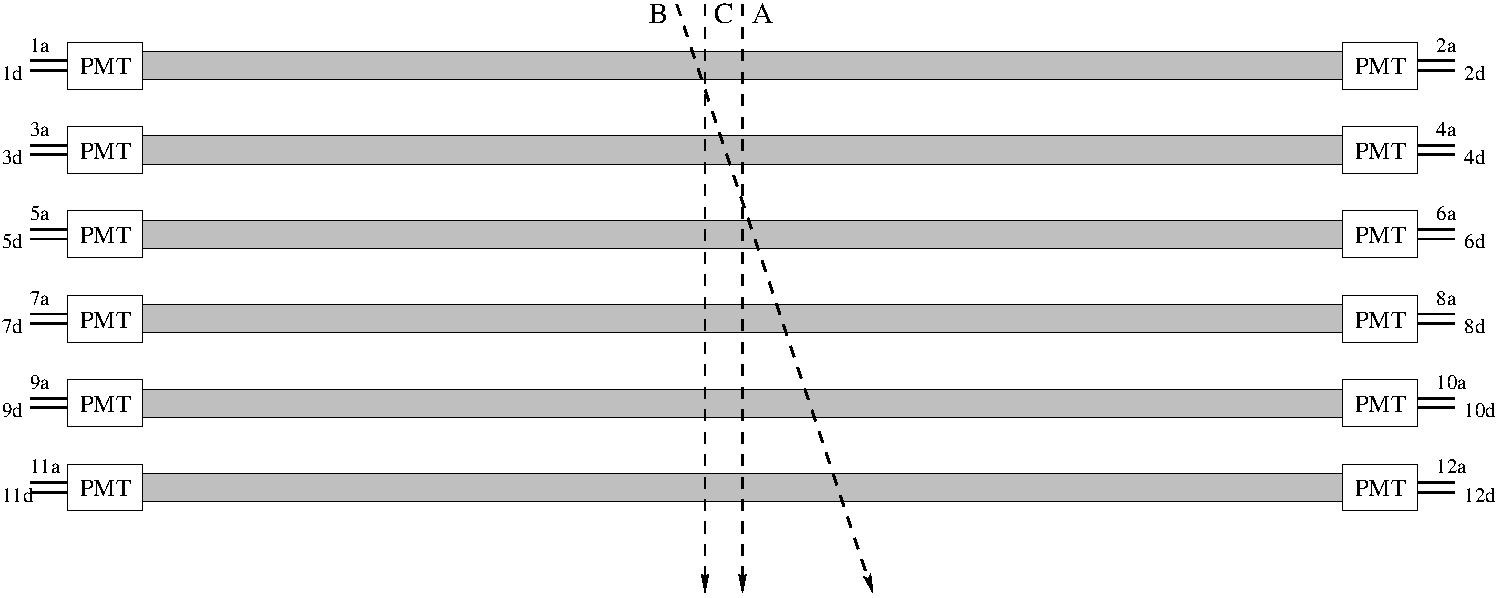
\includegraphics[width=15cm]{gary/fig_gary_six_bar_setup/6bar-setup.pdf}
  \caption{Depiction of six bar method setup.}
  \label{6bar-setup}
\end{figure}

Analogous to the three counters in the three bar method, six
identical-length counters are stacked vertically and equally-spaced,
and events are selected according to the requirement that the
cosmic-ray particle was detected by all six counters.  Labeling the
counters 1 through 6, starting with the top counter, and using the
notation (top, middle, bottom) to represent the counters involved in
each three bar measurement, the three-bar measurements performed are:
(1,2,3), (2,3,4), (3,4,5), (4,5,6), (1,3,5), and (2,4,6).  These are
the only possible combinations of three counters in which the spacing
between adjacent counters is the same.

\begin{figure}[H]
  \centering
  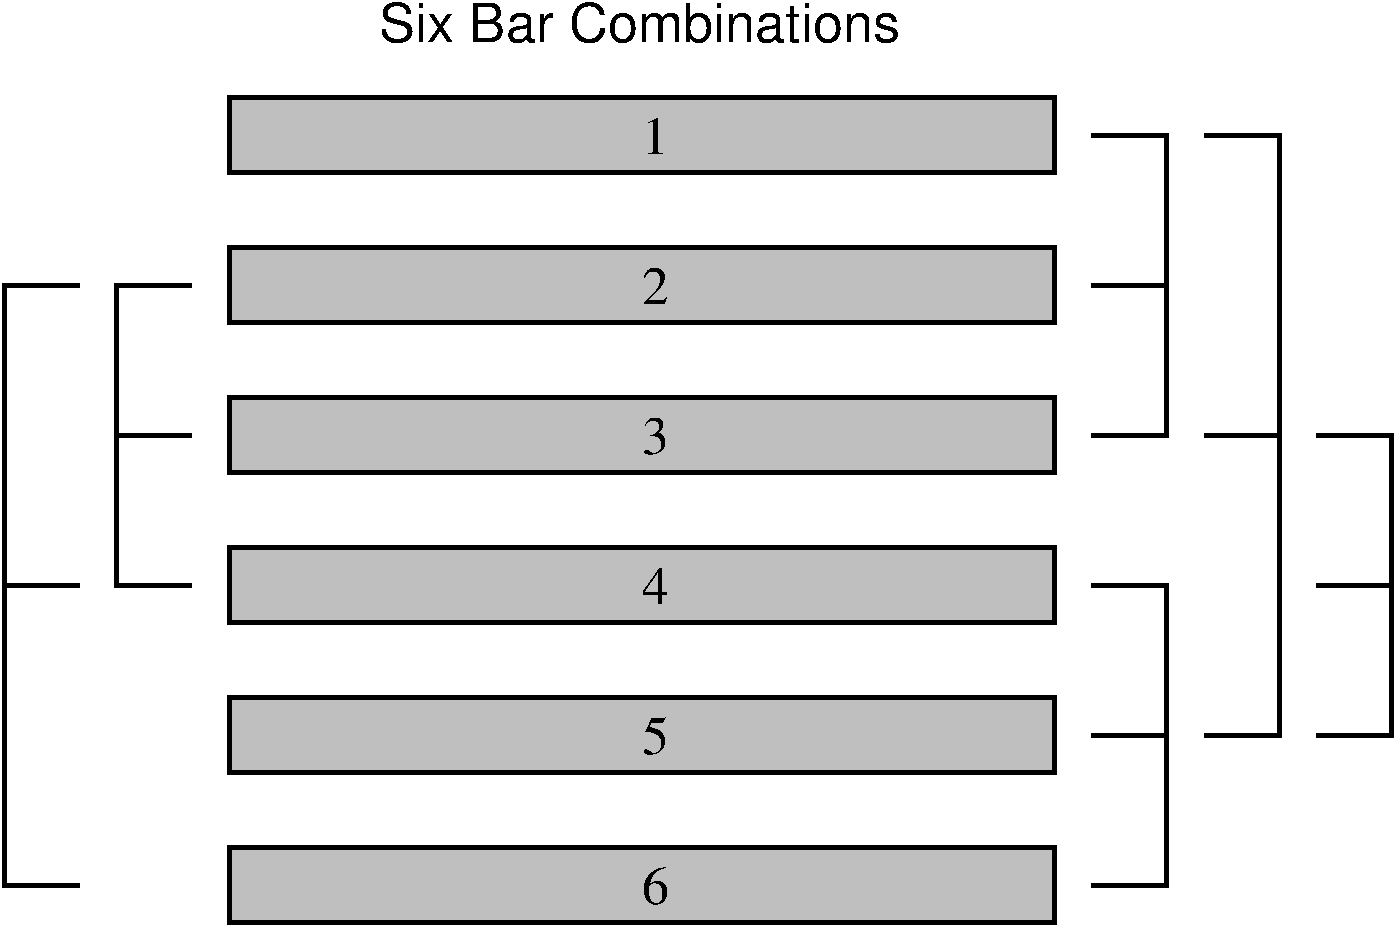
\includegraphics[width=15cm]{gary/fig_gary_six_bar_combinations/6bar-combinations.pdf}
  \caption{Depiction of which three bar combinations are selected for
    the six bar method.}
  \label{6bar-combinations}
\end{figure}

Using $t_n$ for the cosmic-ray interaction times through the
$n\mathrm{th}$ counter, the three-bar method observables for each of
the six combinations of three counters are given by:

\begin{equation}
  T_{(1,2,3)} = (t_1 + t_3)/2 - t_2,
\end{equation}
\begin{equation}
  T_{(2,3,4)} = (t_2 + t_4)/2 - t_3,
\end{equation}
\begin{equation}
  T_{(3,4,5)} = (t_3 + t_5)/2 - t_4,
\end{equation}
\begin{equation}
  T_{(4,5,6)} = (t_4 + t_6)/2 - t_5,
\end{equation}
\begin{equation}
  T_{(1,3,5)} = (t_1 + t_5)/2 - t_3,
\end{equation}
\begin{equation}
  T_{(2,4,6)} = (t_2 + t_6)/2 - t_4.
\end{equation}

Applying error propagation to the above equations, this system of
equations for the counter resolutions follows:

\begin{equation}
  \begin{cases}
    \sigma_{T_{(1,2,3)}}^2 = (\sigma_1^2 + \sigma_3^2)/4 + \sigma_2^2\\
    \sigma_{T_{(2,3,4)}}^2 = (\sigma_2^2 + \sigma_4^2)/4 + \sigma_3^2\\
    \sigma_{T_{(3,4,5)}}^2 = (\sigma_3^2 + \sigma_5^2)/4 + \sigma_4^2\\
    \sigma_{T_{(4,5,6)}}^2 = (\sigma_4^2 + \sigma_6^2)/4 + \sigma_5^2\\
    \sigma_{T_{(1,3,5)}}^2 = (\sigma_1^2 + \sigma_5^2)/4 + \sigma_3^2\\
    \sigma_{T_{(2,4,6)}}^2 = (\sigma_2^2 + \sigma_6^2)/4 + \sigma_4^2
  \end{cases}
\end{equation}

Written in matrix form, the system of equations is:

\begin{equation}
  \left[\begin{array}{c}
      \sigma_{T_{(1,2,3)}}^2 \\
      \sigma_{T_{(2,3,4)}}^2 \\
      \sigma_{T_{(3,4,5)}}^2 \\
      \sigma_{T_{(4,5,6)}}^2 \\
      \sigma_{T_{(1,3,5)}}^2 \\
      \sigma_{T_{(2,4,6)}}^2 \\
    \end{array}
    \right]
  = \left[ \begin{array}{cccccc}
      \frac{1}{4} & 1 & \frac{1}{4} & 0 & 0 & 0 \\
      0 & \frac{1}{4} & 1 & \frac{1}{4} & 0 & 0 \\
      0 & 0 & \frac{1}{4} & 1 & \frac{1}{4} & 0 \\
      0 & 0 & 0 & \frac{1}{4} & 1 & \frac{1}{4} \\
      \frac{1}{4} & 0 & 1 & 0 & \frac{1}{4} & 0 \\
      0 & \frac{1}{4} & 0 & 1 & 0 & \frac{1}{4}\\
    \end{array}
    \right]
  \left[
    \begin{array}{c}
      \sigma_1^2 \\
      \sigma_2^2 \\
      \sigma_3^2 \\
      \sigma_4^2 \\
      \sigma_5^2 \\
      \sigma_6^2 \\
    \end{array}
    \right]
\end{equation}

Since the determinant of the coefficient matrix is non-zero
($81/1024$), the system is independent and can be solved to yield the
\(\sigma_i^2\) by one of the many available techniques to solve a
linear system of equations.

\subsection{Refinement of the Six Bar Method}
The method as stated above suffers from a fundamental asymmetry in the
way the counters are used in the calculations (as shown in the table
below): The inner two counters are each involved in four of the $T_k$,
whereas the next outer two are only necessary for three each and the
outer most are only used in two of the $T_k$; this causes some
counters to have a stronger influence on the computed counter
resolutions than others.  In practice this results in large
fluctuations in the computed counter resolutions, but can be helped
with a slight modification to the method.\\

\begin{tabular}[c]{c || c || c}
  Counter & \# of Dependent $T_k$ & Dependent Combinations\\ \hline
  1 & 2 & (1,2,3), (1,3,5)\\
  2 & 3 & (1,2,3), (2,3,4),(2,4,6)\\
  3 & 4 & (1,2,3), (2,3,4), (3,4,5), (1,3,5)\\
  4 & 4 & (2,3,4), (3,4,5), (4,5,6), (2,4,6)\\
  5 & 3 & (3,4,5), (4,5,6), (1,3,5)\\
  6 & 2 & (4,5,6), (2,4,6)\\
\end{tabular}\\

To remedy this, two consecutive 6-bar measurements are run instead of
one, with the second measurement having the counters stacked in a
different order (known as the \textit{complementary ordering}).  The
order was selected to make the number of equations containing each
counter resolution the same, and is described by the permutation, from
top to bottom, (3,2,1,6,5,4).

\begin{figure}[H]
  \centering
  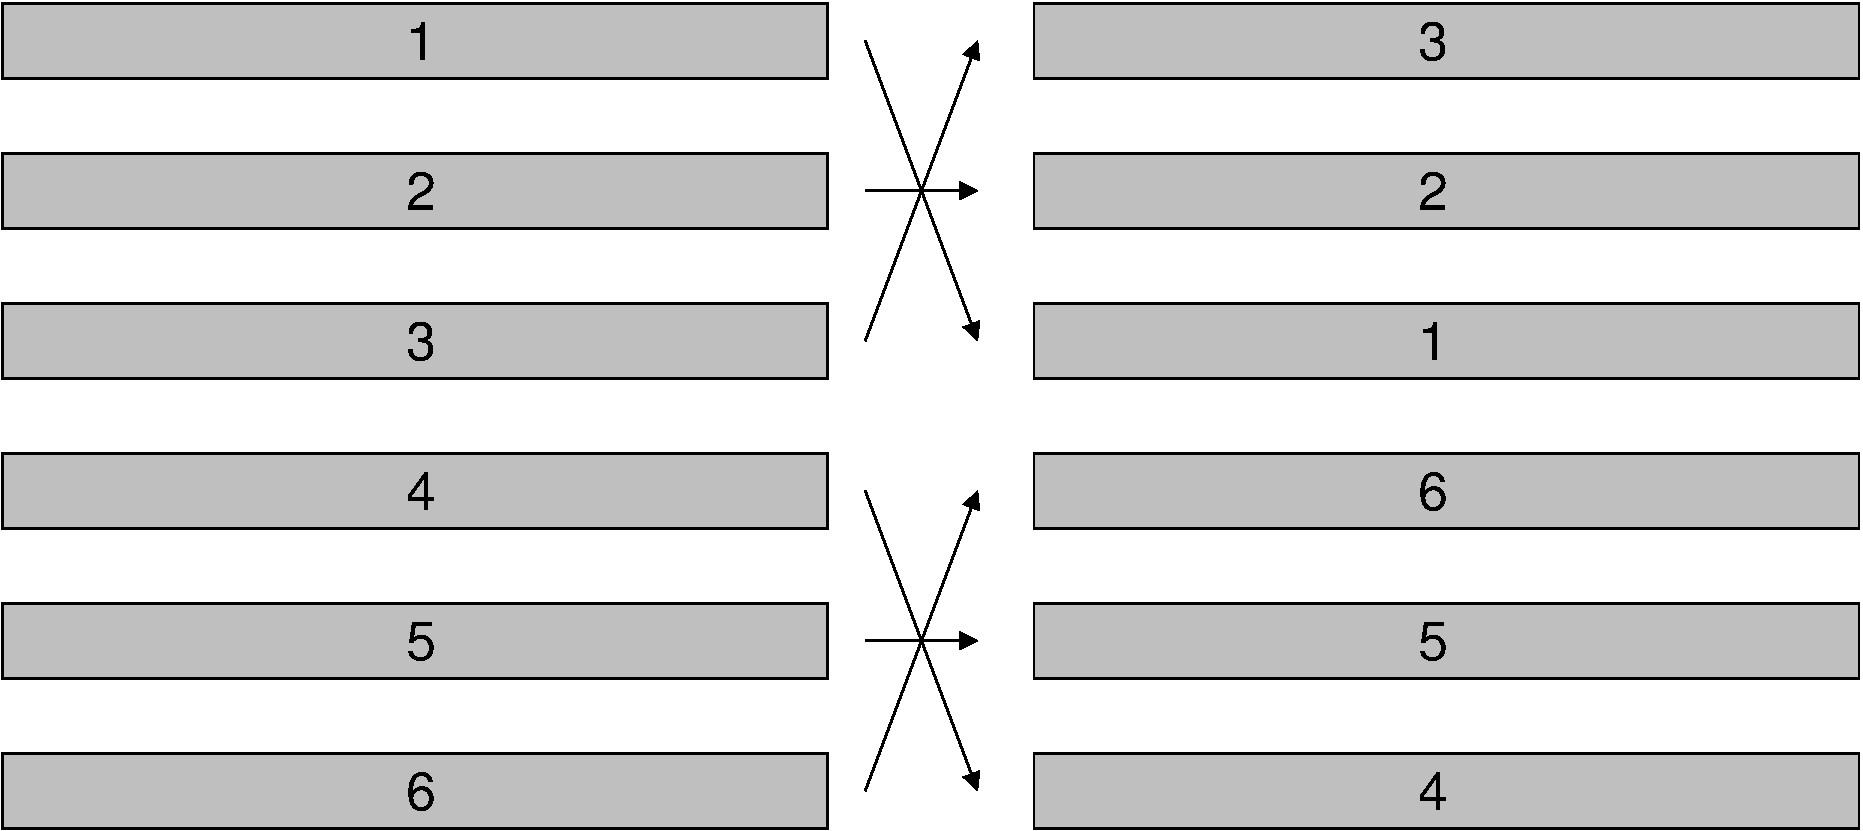
\includegraphics[width=15cm]{gary/fig_gary_six_bar_refinement/complementary.pdf}
  \caption{Rearrangement of the six counters for the complementary
    measurement.}
  \label{complementary}
\end{figure}

The additional three bar observables are

\begin{equation}
  T_{(3,2,1)} = (t_3 + t_1)/2 - t_2,
\end{equation}
\begin{equation}
  T_{(2,1,6)} = (t_2 + t_6)/2 - t_1,
\end{equation}
\begin{equation}
  T_{(1,6,5)} = (t_1 + t_5)/2 - t_6,
\end{equation}
\begin{equation}
  T_{(6,5,4)} = (t_6 + t_4)/2 - t_5,
\end{equation}
\begin{equation}
  T_{(3,1,5)} = (t_3 + t_5)/2 - t_1,
\end{equation}
\begin{equation}
  T_{(2,6,4)} = (t_2 + t_4)/2 - t_6,
\end{equation}

leading to the following over-constrained system of equations for the
individual counter resolutions,

\begin{equation}
  \begin{cases}
    \sigma_{T_{(1,2,3)}}^2 = (\sigma_1^2 + \sigma_3^2)/4 + \sigma_2^2\\
    \sigma_{T_{(2,3,4)}}^2 = (\sigma_2^2 + \sigma_4^2)/4 + \sigma_3^2\\
    \sigma_{T_{(3,4,5)}}^2 = (\sigma_3^2 + \sigma_5^2)/4 + \sigma_4^2\\
    \sigma_{T_{(4,5,6)}}^2 = (\sigma_4^2 + \sigma_6^2)/4 + \sigma_5^2\\
    \sigma_{T_{(1,3,5)}}^2 = (\sigma_1^2 + \sigma_5^2)/4 + \sigma_3^2\\
    \sigma_{T_{(2,4,6)}}^2 = (\sigma_2^2 + \sigma_6^2)/4 + \sigma_4^2\\
    \sigma_{T_{(3,2,1)}}^2 = (\sigma_3^2 + \sigma_1^2)/4 - \sigma_2^2\\
    \sigma_{T_{(2,1,6)}}^2 = (\sigma_2^2 + \sigma_6^2)/4 - \sigma_1^2\\
    \sigma_{T_{(1,6,5)}}^2 = (\sigma_1^2 + \sigma_5^2)/4 - \sigma_6^2\\
    \sigma_{T_{(6,5,4)}}^2 = (\sigma_6^2 + \sigma_4^2)/4 - \sigma_5^2\\
    \sigma_{T_{(3,1,5)}}^2 = (\sigma_3^2 + \sigma_5^2)/4 - \sigma_1^2\\
    \sigma_{T_{(2,6,4)}}^2 = (\sigma_2^2 + \sigma_4^2)/4 - \sigma_6^2
  \end{cases}
\end{equation}

and in matrix form,

\begin{equation}
  \left[\begin{array}{c}
      \sigma_{T_{(1,2,3)}}^2 \\
      \sigma_{T_{(2,3,4)}}^2 \\
      \sigma_{T_{(3,4,5)}}^2 \\
      \sigma_{T_{(4,5,6)}}^2 \\
      \sigma_{T_{(1,3,5)}}^2 \\
      \sigma_{T_{(2,4,6)}}^2 \\

      \sigma_{T_{(3,2,1)}}^2 \\
      \sigma_{T_{(2,1,6)}}^2 \\
      \sigma_{T_{(1,6,5)}}^2 \\
      \sigma_{T_{(6,5,4)}}^2 \\
      \sigma_{T_{(3,1,5)}}^2 \\
      \sigma_{T_{(2,6,4)}}^2 \\
    \end{array}
    \right]
  = \left[ \begin{array}{cccccc}
      \frac{1}{4} & 1 & \frac{1}{4} & 0 & 0 & 0 \\
      0 & \frac{1}{4} & 1 & \frac{1}{4} & 0 & 0 \\
      0 & 0 & \frac{1}{4} & 1 & \frac{1}{4} & 0 \\
      0 & 0 & 0 & \frac{1}{4} & 1 & \frac{1}{4} \\
      \frac{1}{4} & 0 & 1 & 0 & \frac{1}{4} & 0 \\
      0 & \frac{1}{4} & 0 & 1 & 0 & \frac{1}{4}\\

      \frac{1}{4} & 1 & \frac{1}{4} & 0 & 0 & 0 \\
      1 & \frac{1}{4} & 0 & 0 & 0 & \frac{1}{4} \\
      \frac{1}{4} & 0 & 0 & 0 & \frac{1}{4} & 1 \\
      0 & 0 & 0 & \frac{1}{4} & 1 & \frac{1}{4} \\
      1 & 0 & \frac{1}{4} & 0 & \frac{1}{4} & 0 \\
      0 & \frac{1}{4} & 0 & \frac{1}{4} & 0 & 1 \\
    \end{array}
    \right]
  \left[
    \begin{array}{c}
      \sigma_1^2 \\
      \sigma_2^2 \\
      \sigma_3^2 \\
      \sigma_4^2 \\
      \sigma_5^2 \\
      \sigma_6^2 \\
    \end{array}
    \right],
\end{equation}

or just

\begin{equation}
  \vec{T} = \hat{A} \vec{\sigma}.
\end{equation}

%I need to add some pictures showing the results of using the combined
%measurements vs. just the original six bar method.
In the combined over-constrained system of equations, each counter
resolution occurs in six equations.  This modification makes the
method noticeably more stable when computing the individual counter
resolutions.  As the new system of equations is over-constrained, the
best estimator for the solution to the system is given by the method
of linear least-squares.  Linear least-squares consists of solving the
following equation for \(\vec{\sigma}\):

\begin{equation}
  (\hat{A}^T \hat{A}) \vec{\sigma} = \hat{A}^T \vec{T}.
\end{equation}

%% Need to add figure showing how normal+complementary is more stable
%% than just normal or complementary ordering (independent of
%% statistics since normal+complementary has more statistics than
%% either normal or complementary alone).

\subsection{Electronics}

The primary electronic subsystem components relevant to FTOF12 time resolution are discriminators, time-to-digital converters (TDC), and charge-to-digital converters (QDC).  Each anode PMT pulse of sufficient amplitude generates a logic signal by way of a discriminator, and the logic signal's time of arrival is measured by a TDC.  In parallel, the corresponding dynode PMT pulse is integrated by a QDC.  In the case of FTOF12's fixed-risetime PMT signals, the time required for the incoming signal to reach the discriminator threshold (timewalk) can be subtracted according to the signal size, which is proportional to the corresponding QDC value.  The TDC sets the fundamental lower limit on the time resolution measurement, the discriminator introduces time variations primarily through timewalk, and the QDC provides information that allows for timewalk correction.  Accordingly, the properties of each of these components are crucial to achieving optimal time resolution.

\subsubsection{TDC testing}

{\it Important figures:\\
integral nonlinearity (INL) -- cable delay plots \\
differential nonlinearity (DNL) -- white histogram, channel width distribution\\
intrinsic time resolution\\
dithering mode on versus off\\
}



The properties of the TDC determine the most basic unit of time resolution. Resolution, differential nonlinearity (DNL), and integral nonlinearity (INL), were measured for common-start CAMAC modules (Phillips Scientific PS7186 and Caen C414) and a newer pipeline VME module (Caen V1290N). Neither CAMAC module met the manufacturer's specifications, but the Caen VME module V1290N performed acceptably, which was one factor in the choice to use VME during our prototype development.  Ultimately, however, the pipeline class of TDC is required for a more basic reason: it allows for the decoupling of the coincidence trigger from the timing trigger, which removes all electronic logic system contributions other than the discriminator from the time resolution.

In order to determine the DNL profile of each module, a random start signal and periodic stop signal are fed to the TDC. The stop signal arrives at the TDC in any fixed-width time interval with equal probability.  Thus, after a large number of events, a uniform distribution of counts per time interval (bin) is expected in the ideal case. Deviations from the ideal result minus statistical noise reflect the TDC's DNL.

\begin{figure}[]
\centering
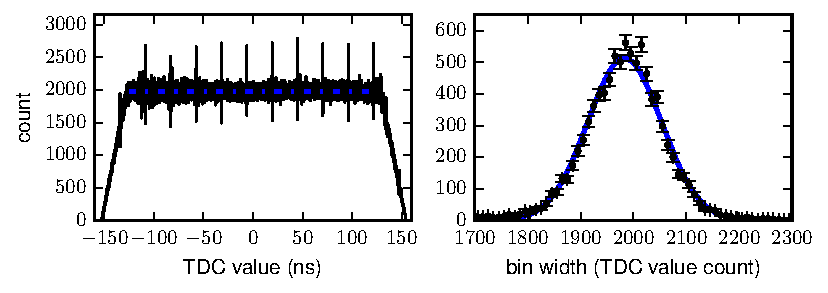
\includegraphics[]{evan/fig_evan_tdc_testing/tdc_dnl_v1290n.pdf} %{cDNL.pdf}
\caption{The DNL histogram (left) deviates from an ideal uniform distribution, indicated by the dotted line, with a standard deviation of 70 counts (right), so the relative nonlinearity is $\frac{70}{1983} = 3.5\%$. After compensating for the statistical contribution of $\frac{\sqrt{1983}}{1983} = 2.2\%$, the relative DNL is $2.7\%$. The sloped edges result from the $25\:ns$ variability in the V1290N's timing window with respect to the trigger. The periodic needles, again at $25\:ns$ intervals, result from INL compensation on the TDC chip level.\cite{v1290n-man} The additional interference at TDC value $0$ results from crosstalk between the two signals.\label{fig:tdcDNL}}
\end{figure}

A radioactive source of Sr-90, placed on a counter, provides the random signals, which are converted to NIM logic signals by a leading edge discriminator (Phillips Scientific 705) for timing. In parallel, a timing unit (Phillips Scientific 794) provides logic pulses with a period greater than the TDC full range for the common-start CAMAC TDCs and a period of $200\:ns$ for the pipeline VME TDC. The random signal serves as the reference signal, and the periodic signal, sent to all channels via a logic fan in/out (LeCroy 429A), serves as the channel-specific stop. A TDC value distribution and its corresponding bin-width distribution are histogrammed in Fig.$\:$\ref{fig:tdcDNL}, and for comparison, the DNL histograms of PS7186 and C414 are illustrated in Fig.$\:$\ref{fig:tdcDNLcamac}.

\begin{figure}[]
\centering
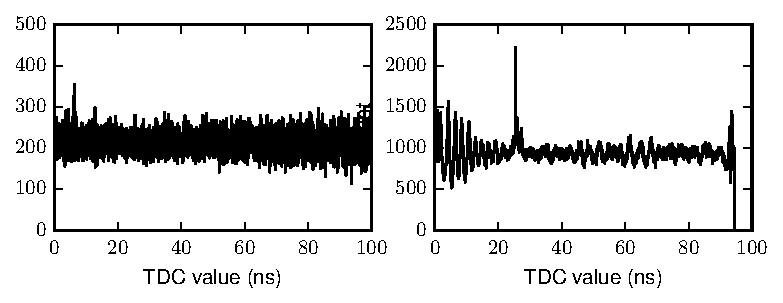
\includegraphics[width=0.8\textwidth]{evan/fig_evan_tdc_testing/tdc_dnl_camac.pdf} %{dnl_camac.pdf}
\caption{DNL histograms for the Phillips Scientific 7186 (left) and the Caen 414 (right), compared with that of the Caen V1290N (Fig.$\:$\ref{fig:tdcDNL}, left), illustrate different nonlinearity signatures. The PS7186 and C414 are 12-bit CAMAC modules with limited ranges. The entire $100\:ns$ range (12-bit) is usable in the PS7186, but the high nonlinearity below bin 1100 of the C414 restricts the usable range to only about $60\:ns$.\label{fig:tdcDNLcamac}}
\end{figure}

\begin{figure}[]
\centering
\includegraphics[width=0.8\textwidth, height=2.5in]{evan/fig_evan_tdc_testing/placeholder.eps} %{tdc_c414_cableDelays.pdf}
\includegraphics[width=0.8\textwidth, height=2.5in]{evan/fig_evan_tdc_testing/placeholder.eps} %{tdc_cal.pdf}
\caption{Typical TDC calibration results illustrated for the Caen C414. Two copies of the same signal are used as start and stop times, with the latter being delayed with measured cable lengths in $5\:ns$ increments (top). The typical peak width corresponds to $\sigma=0.7\:bins$. The mean TDC value of each peak is plotted with its corresponding measured delay (bottom) to get the TDC sensitivity and offset (parameters $p1$ and $p0$, respectively).\label{fig:tdcDelays}}
\end{figure}

Calibration of the TDCs was accomplished by applying variable, oscilloscope-measured cable delays in $5\:ns$ increments. Figure$\:$\ref{fig:tdcDelays} demonstrates the calibration procedure where, in the illustrated case of the Caen C414, the average bin width is $25.11\:ps$ with an offset of $2.8\:ns$. Each $5ns$-interval peak includes 1000 entries and has a width corresponding to $0.6\:\textrm{bins}<\sigma<0.8\:\textrm{bins}$. Results for each TDC are tabulated in Table$\:$\ref{tab:TDC}.

\begin{table}[]
\centering
\caption{TDC Summary.}
\begin{tabular}{c r r r r r r }
\hline
Model & DNL$_{\sigma}$ & DNL$_{max}$ & Range(ns) & Offset(ns) & Bin Size(ps) & Resolution(ps) \\
\hline\hline
PS7186 & 9.4\% & 48.9\% & 100 & 18-21 & 24.98 & 19.0 \\
C414 & 6.5\% & 135.6\% & 72 & 0-5 & 25.11 & 17.5 \\
V1290N & 2.7\% & 41.1\% & N/A & N/A & 24.75 & 32.5 \\
\hline
\end{tabular}
\label{tab:TDC}
\end{table}


\subsubsection{QDC testing}

{\it Note:
variable offset (motivating external DC offset)\\
dynamic range\\
DNL/INL (*?)\\
}

For the purpose of time resolution measurements, the QDC is only used in correcting for signal time of arrival, so calibrating the QDC values to an absolute energy scale of energy deposited is unnecessary.  However, identifying the module's ground and the system charge offset (the \textit{zero}) is crucial. For the prototype testing, the Caen V792N QDC\cite{v792n-man} (integrating QDC) was tested and calibrated such that the zero was in an acceptable range using a combination of the module's software-adjustable pedestal and an externally applied DC offset. To identify the full range of the QDC's pedestal, a fixed-width integration gate ($T_{gate}=100\:ns$) and measured DC offsets are applied to a ground signal and integrated for various pedestal settings (Fig.$\:$\ref{fig:qdcTest}).

\begin{figure}[ht]
%\includegraphics[width=2.5in]{QdcTest1.png}
\includegraphics[width=2.5in]{evan/fig_evan_qdc_testing/placeholder.pdf}
\caption{A fixed-width integration gate, $T_{gate}$, and variable DC offsets, $V_1$-$V_7$ are used to calibrate the QDC, including sensitivity and pedestal measurements.\label{fig:qdcTest}}
\end{figure}

\begin{figure}[ht]
%\includegraphics[width=3.5in]{c_15_63_22_55mV.pdf}
\includegraphics[width=3.5in]{evan/fig_evan_qdc_testing/placeholder.pdf}
\caption{An QDC distribution corresponding to a $-22.55\:mV$ offset integrated over $100\:ns$.\label{fig:QDCHist}}
\end{figure}

\begin{figure}
\centering
\mbox{\subfigure[$\:$DC offset versus QDC.]{
%\includegraphics[width=3.1in,height=2.8in]{c_15_63.pdf}\label{fig:offsetVQDC}
\includegraphics[width=3.1in,height=2.8in]{evan/fig_evan_qdc_testing/placeholder.pdf}\label{fig:offsetVQDC}
}\quad
\subfigure[$\:$Pedestal setting versus virtual ground.]{
%\includegraphics[width=3.1in,height=2.8in]{c_15.pdf}\label{fig:pedRange}
\includegraphics[width=3.1in,height=2.8in]{evan/fig_evan_qdc_testing/placeholder.pdf}\label{fig:pedRange}
}}
\caption{(a) For the adjustable pedestal setting of 63, the module has a virtual ground of $-4.6\:mV$ as determined by the QDC zero-crossing. (b) This zero-crossing varies from $\approx 0\:mV$ to $\approx -6\:mV$, so even in this case, an external DC offset is required to push the overall system offset into the active QDC range.}
\end{figure}

%\begin{figure}[ht]
%\includegraphics[width=5in]{c_15_63.pdf}
%\caption{\label{fig:offsetVQDC}}
%\end{figure}

%\begin{figure}[ht]
%\includegraphics[width=5in]{c_15.pdf}
%\caption{\label{fig:pedRange}}
%\end{figure}

Figure$\:$\ref{fig:QDCHist} illustrates the QDC distribution when the pedestal is set to 63 and an external DC offset of $-22.55\:mV$ is applied. Combining such results for various DC offsets, the relationship between the DC offset and QDC value is determined (see Fig.$\:$\ref{fig:offsetVQDC}). The $y$-intercept of the best-fit line indicates the QDC's virtual ground, its pedestal current, with respect to which it integrates incoming signals. Finally, the module's pedestal settings are compared to the corresponding virtual ground values to determine the full range of the adjustable intrinsic pedestal, as shown in Fig.$\:$\ref{fig:pedRange}.

The sensitivity of the QDC is determined from Fig.$\:$\ref{fig:offsetVQDC}, where the best-fit line is cast in terms of charge rather than DC offset as in equation \eqref{f:Q}, where $Q$ corresponds to total charge, $x$ to QDC value (bin), and $R$ to resistance ($50\:\Omega$).
\begin{equation}\label{f:Q}
Q=\left(-4.606\:\frac{mV}{bin}x - 0.0542\:mV\right)\left(\frac{T_{gate}}{R}\right) = -9.2\:\frac{pC}{bin}x - 0.11\:pC
\end{equation}
Accordingly, the V792N's sensitivity of $9.2\:\frac{pC}{bin}$ is consistent with the documented sensitivity of $10\:\frac{pC}{bin}$.

\subsubsection{Discriminator testing}

{\it Note:
constant fraction discriminator (cfd) delay optimization\\
leading edge discriminator (led) threshold optimization\\
cfd vs. led vs. tw-corrected led (*?)\\
}

Discriminators generate logic signals whenever incoming analog signals rise above a preset threshold voltage.  Two classes of discriminators are common:  constant fraction discriminators (CFD) and leading edge discriminators (LED).  CFDs are designed to correct for timewalk by triggering on the sum of the incoming signal and a delayed, attenuated, and inverted duplicate.  LEDs trigger directly on the incoming signal.  Properly tuned CFDs were sufficient for previous time-of-flight applications, but FTOF12 is sensitive to an additional QDC-based timewalk correction to CFD-triggered signals.  Since these additional timewalk corrections would be required in either case, the simpler and less expensive LEDs were used.

In the case of LEDs, the threshold voltage must be optimized to minimize background, maximize good signal acceptance, and reduce time jitter introduced by fine-grained random volage fluctuations.

[TODO: add LED threshold results and discussion!]

\subsection{Time-walk corrections}
\label{sect:Time-walk}

\iffalse
{\it Note:
compare different techniques, including justification of NOT using laser calibration technique\\ $(http://www.jlab.org/Hall-B/notes/clas_notes93/note93-024.pdf)$\\
}
\fi

In order to optimize the time resolution, the time-walk caused by the height dependent timing variation based on Leading Edge Discriminator (LED) measurements has to be corrected. 
These time-walk corrections for the CLAS6 forward time-of-flight detector have been determined by using a laser-based calibration system~\cite{clastof}. This system consists of  four ultraviolet (UV) lasers. The UV light is delivered
to the center of each scintillator via a silica
optical fiber.  The TDC and ADC information
from the injected laser pulses can then be used to calibrate
the overall timing and pulse-height dependent time-walk. 

Due to the improved time resolution of the new CLAS12 time-of-flight panel 1b the previously used method is no longer sufficient and is replased by an in-situ calibration based on the accumulated data itself.
 The reasons for that are the following: a) In contrast to laser light that is delivered only to the center of
the scintillator, physical data are gathered along the whole bar length. The in-situ calibration facilitates a development of position-dependent time-walk corrections, thus improving the time resolution. b) The energy distribution of the particles and the shape of the analog signals that will be used for time-walk corrections will be by definition the same as in experiment, while the laser system injects monochromatic photon pulse with preselected amplitudes not corresponding to the experimental conditions.

During development and construction and before the installation into the CLAS12 detector all scintillation counters have been evaluated and checked using cosmic ray particles. The energy deposit of cosmic muons is relatively close to that of the particles  measured by CLAS12. Moreover, since cosmic muons are distributed homogenously along the scintillator, position-dependent time-walk corrections are applied. As mentioned  in Sec.~\ref{sec:six-bars} the typically used six-bars method demands that six counters are set up one above the other and that all PMT signals are coincide. 

After two days of running a sufficient amount of data was collected for each setup to carry out the analysis. The starting point of time-walk corrections procedure is ADC offsets substruction. Fig.~\ref{fig:offset} (left plot) shows ADC distribution zoomed in offset region. The offset peak position marked by red line was substracted from ADC values event by event. Shifted distribution is shown on the right plot of Fig.~\ref{fig:offset}. For further analysis all events that correspond to the offset peak were cut away.  


\begin{figure}[]
\begin{center}
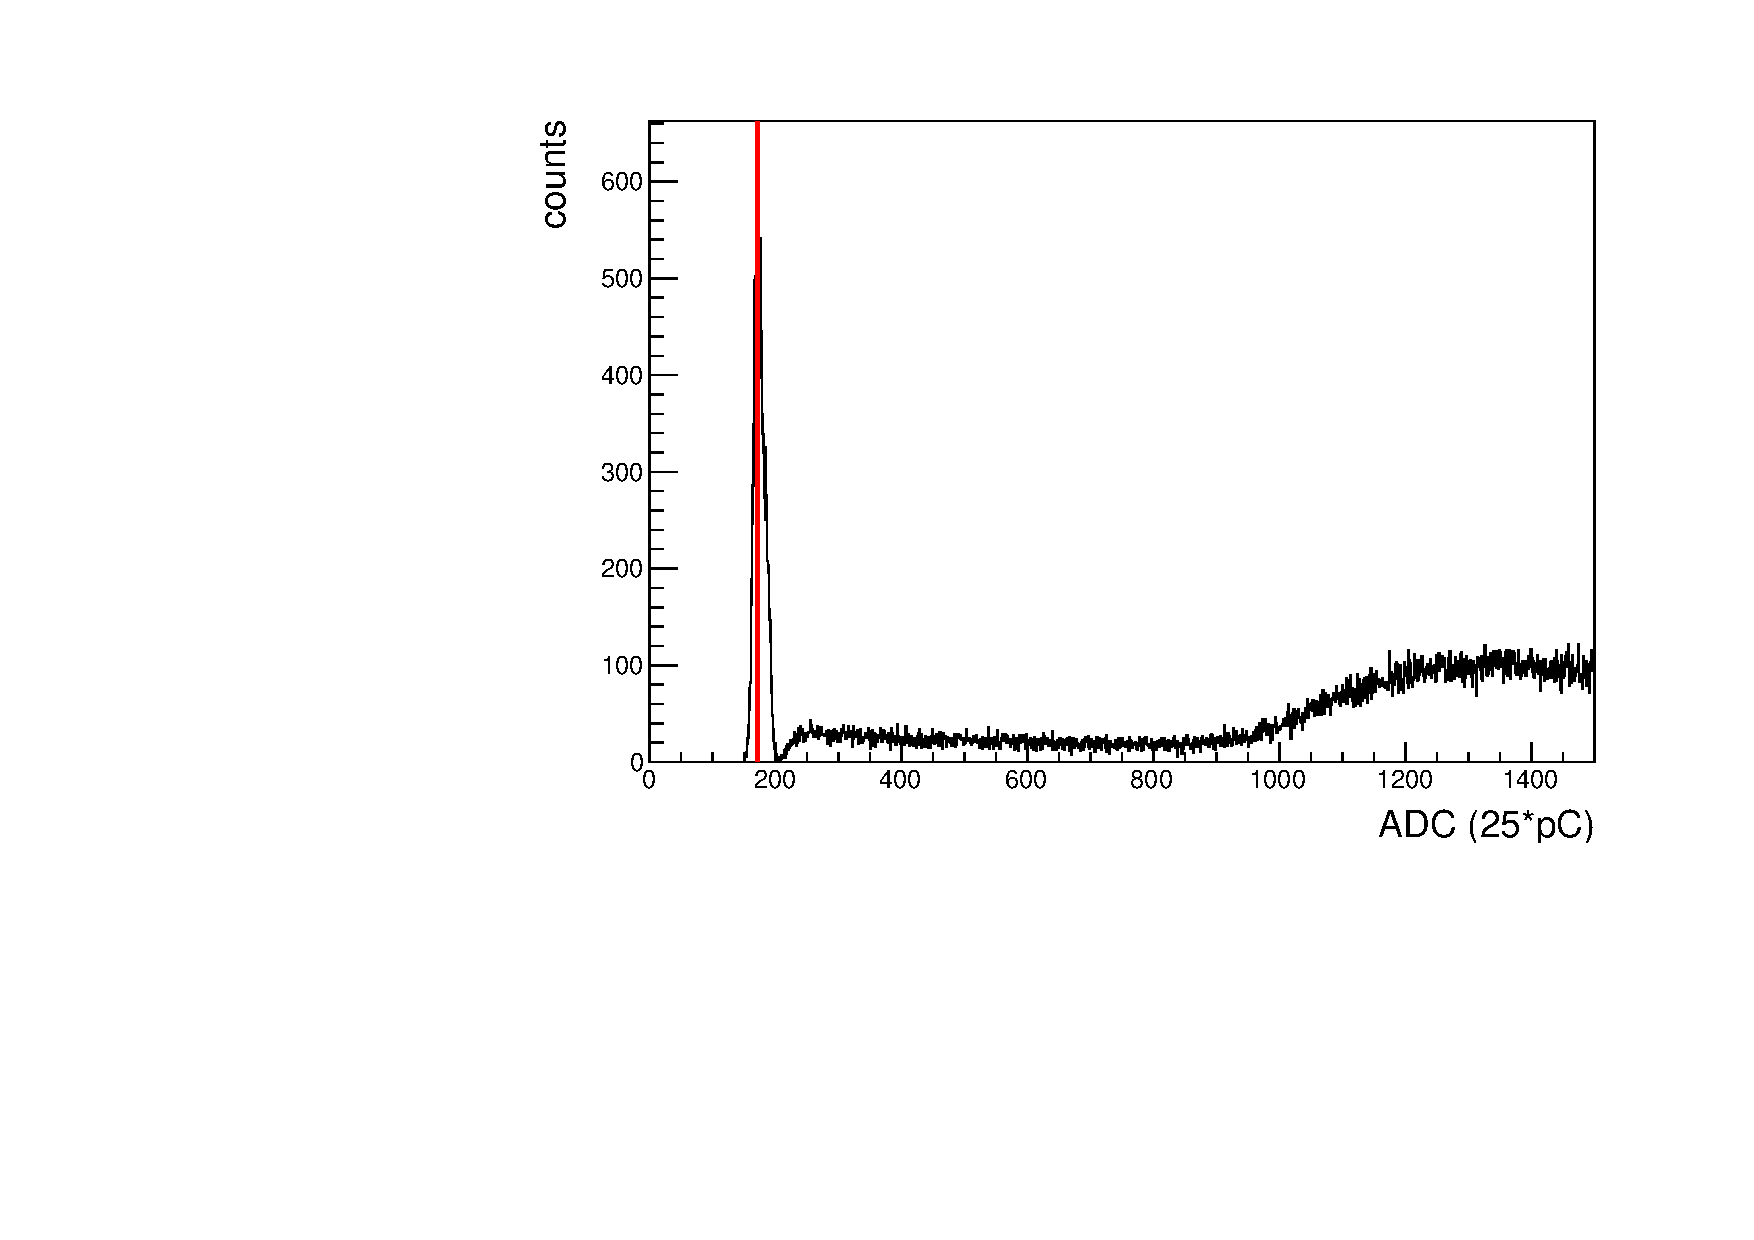
\includegraphics[width=3in]{gleb/fig_gleb_time_walk/offset.pdf}
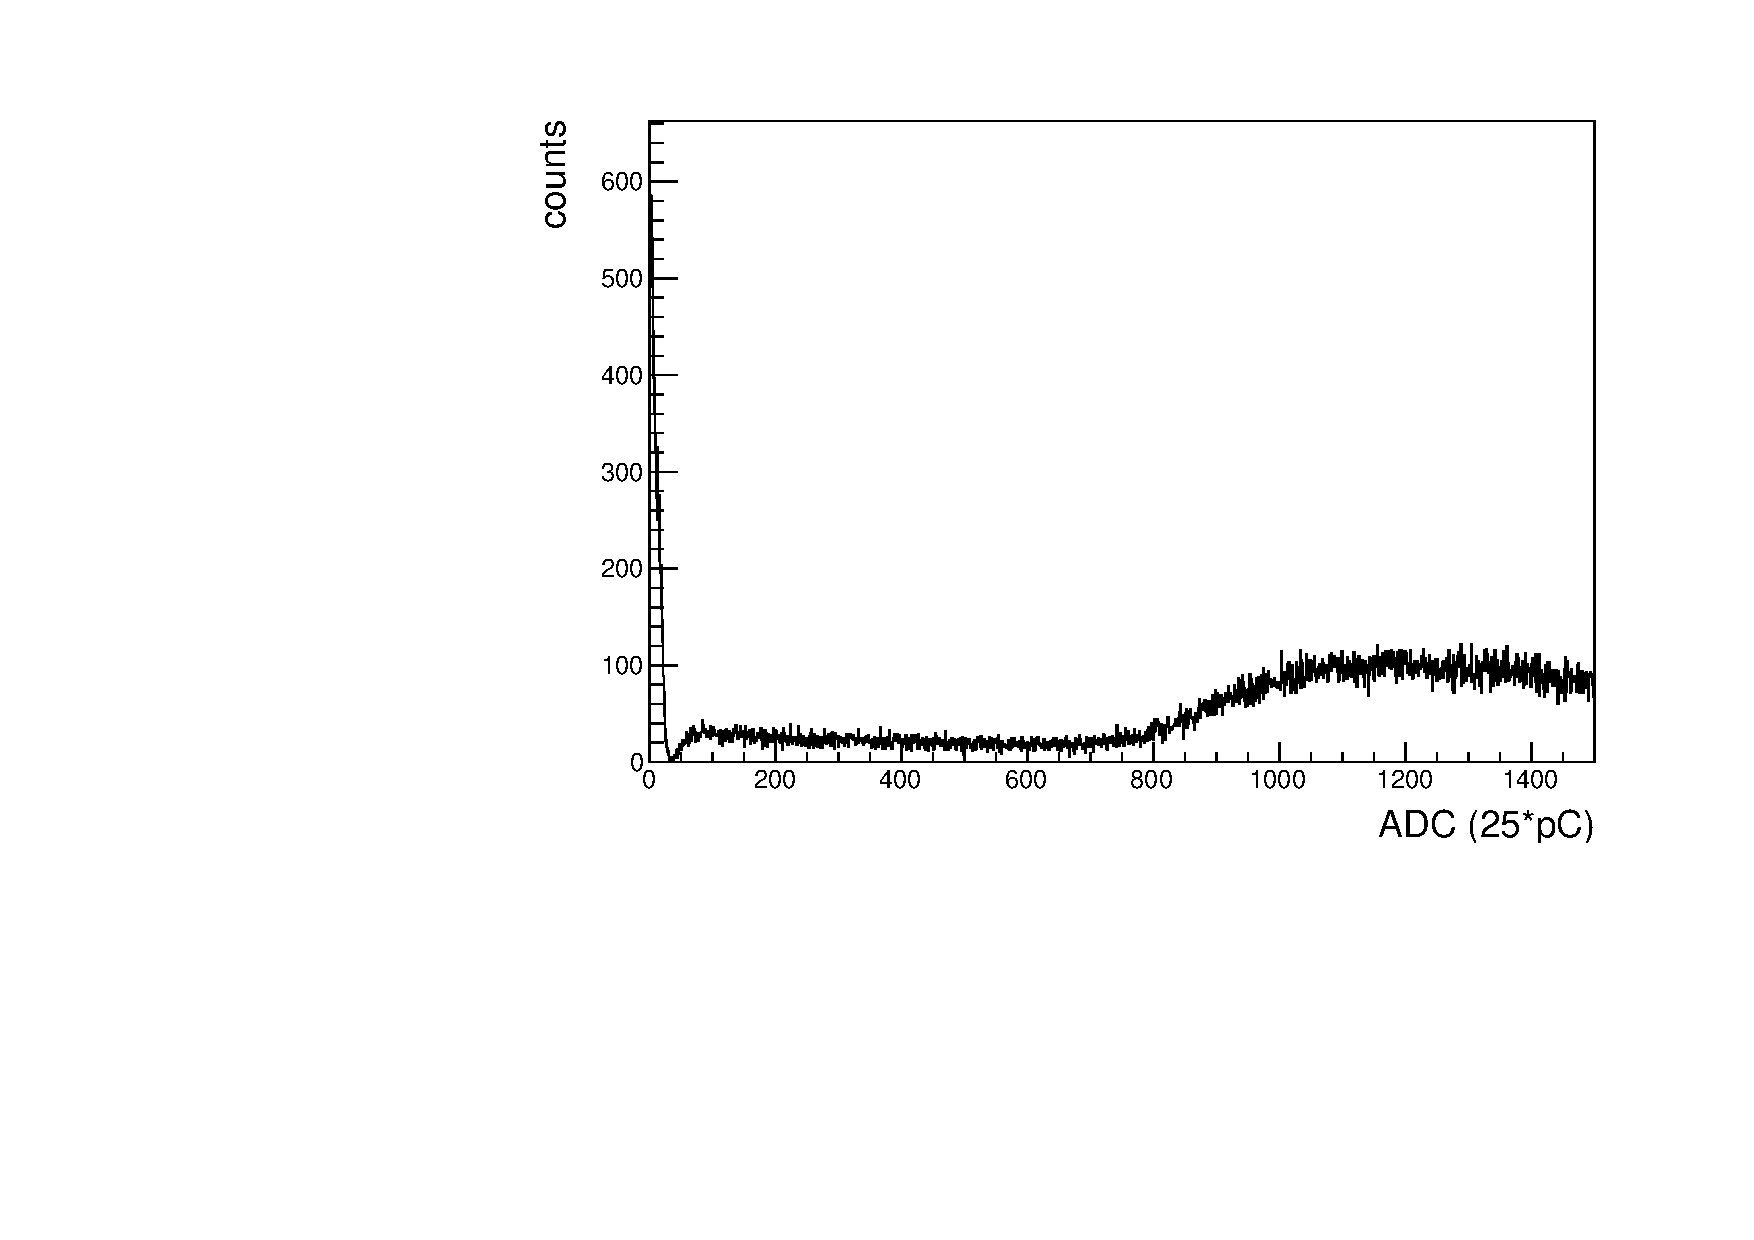
\includegraphics[width=3in]{gleb/fig_gleb_time_walk/offset_shifted.pdf}
\caption{ADC distribution zoomed in offset region before (left plot) and after (right plot) ADC offset substraction. Vertical red line on the left plot shows the position of the offset peak. \label{fig:offset}}
\end{center}
\end{figure}

The next step is vertical tracks selection that is not necessary for the method itself, but needed since position-dependent procedure is going to be applied. For that purpose the TDC difference between left and right PMTs for  bottom counter versus the same quantity for the top one (see Fig.~\ref{fig:vert_cut}) were plotted. These differences are divided over two since at that case they correspond to the bar length divided by effective speed of light. To determine the position of the red line (see Fig.~\ref{fig:vert_cut}) one dimentional distribution of the quantity $x - y$ was plotted (see Fig.~\ref{fig:diff_between_diff}), where $x = (tdc1-tdc2)/2$ and $y = (tdc11-tdc12)/2$. These quantities correspond to the $x$ and $y$ axes of the two dimentional plot Fig.~\ref{fig:vert_cut}. This one dimentional distribution was fitted by gaussian to determine the mean value $M$ (see Fig.~\ref{fig:diff_between_diff}). The line with equation $y = x + M$ is drawn by red on Fig.~\ref{fig:vert_cut}.For analysis the whole bar length was divided into the bins approximatly 3 cm width each. The range over x-axis that correspond to the scintillator length was divided into the same number of bins. 
Bin size over y-axis was determined by intersections of boundaries of the bin over x-axis with red line.
Events within rectangular area (shown in white on Fig.~\ref{fig:vert_cut}) were selected for further analysis.  
All steps described below correspond to one particular bin.

\begin{figure}[]
\begin{center}
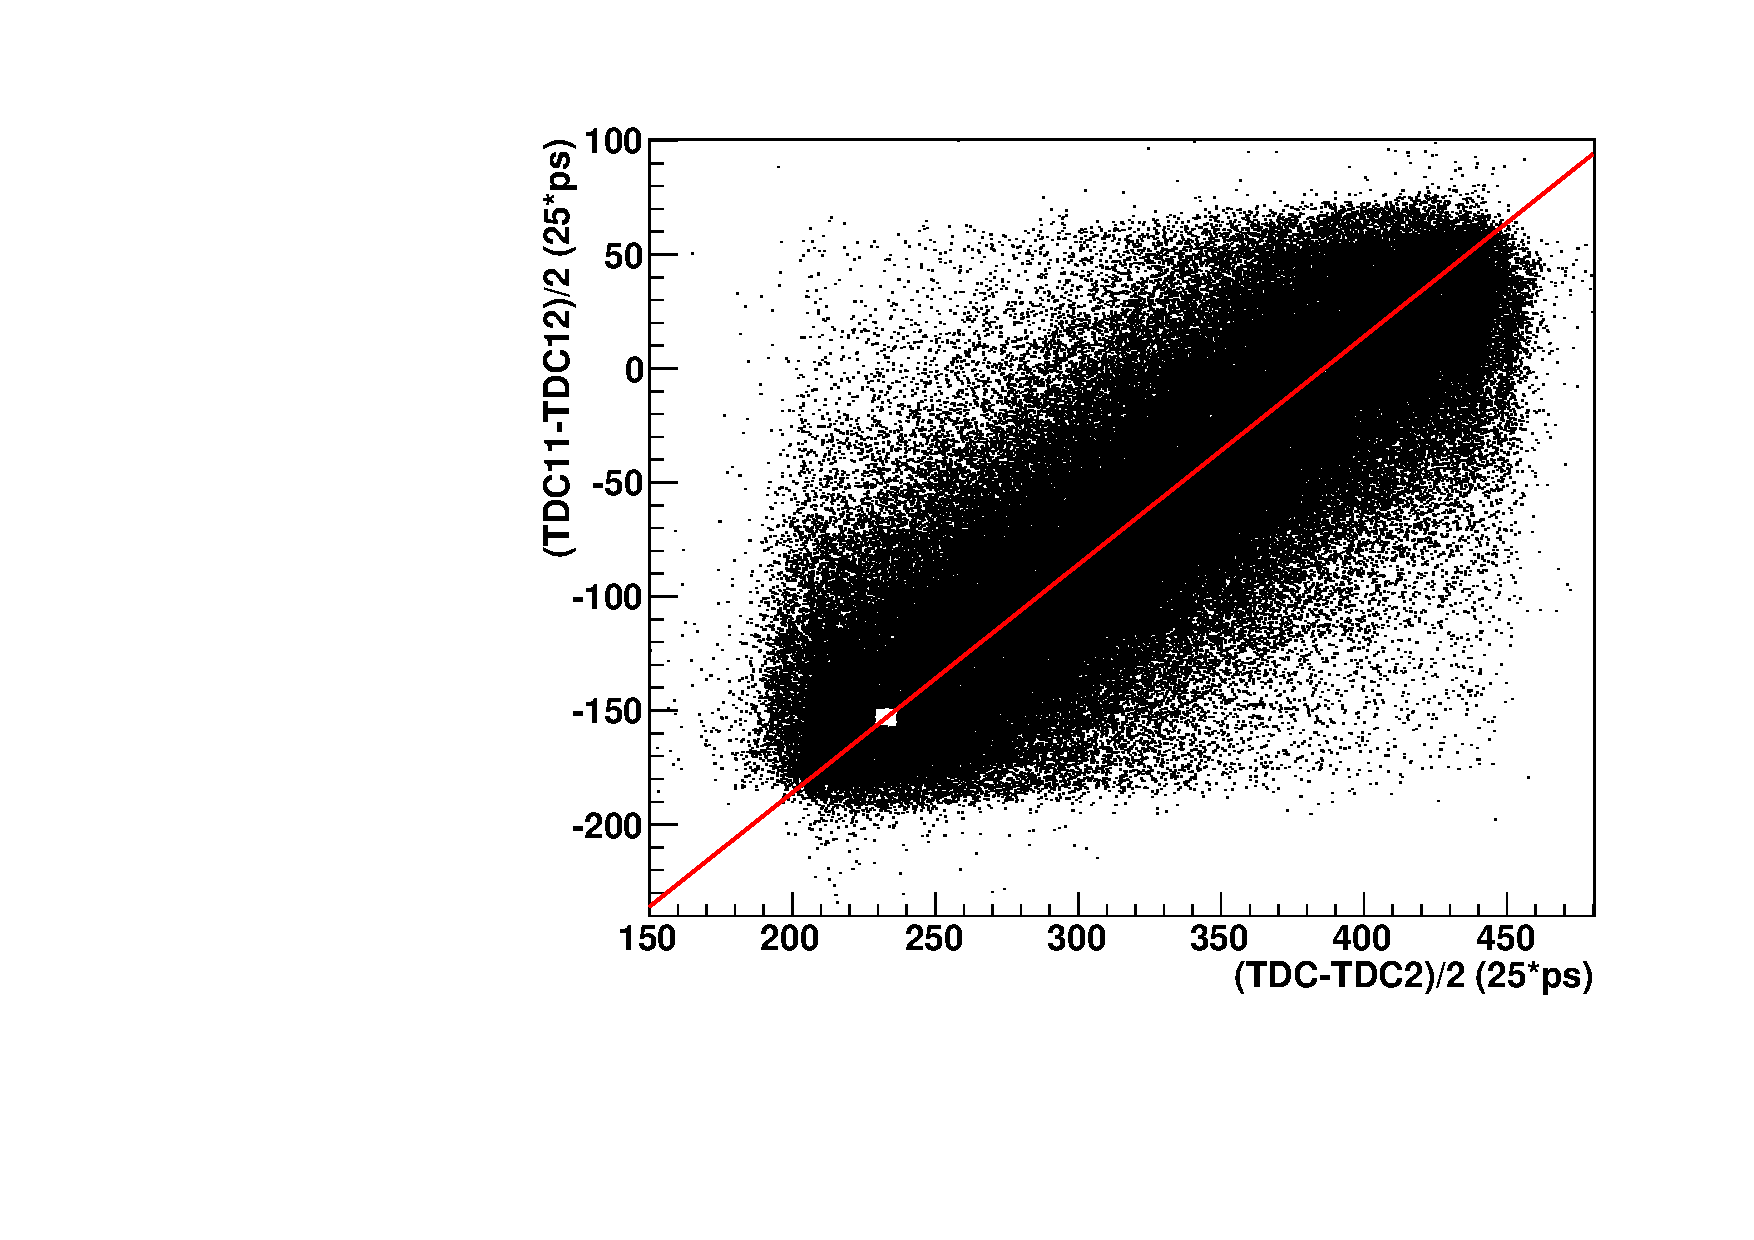
\includegraphics[width=3in]{gleb/fig_gleb_time_walk/vert_cut.pdf}
\caption{TDC difference between left and right PMTs for  bottom counter versus the same quantity for the top one. Plot corresponds to the bars 81cm long from the set number eleven. The position of red line is determined by fitting of distribution shown on Fig.~\ref{fig:diff_between_diff}. Rectangular area shown in white is one of the bins that was used for time-walk parameters determination. \label{fig:vert_cut}}
\end{center}
\end{figure}

\begin{figure}[]
\begin{center}
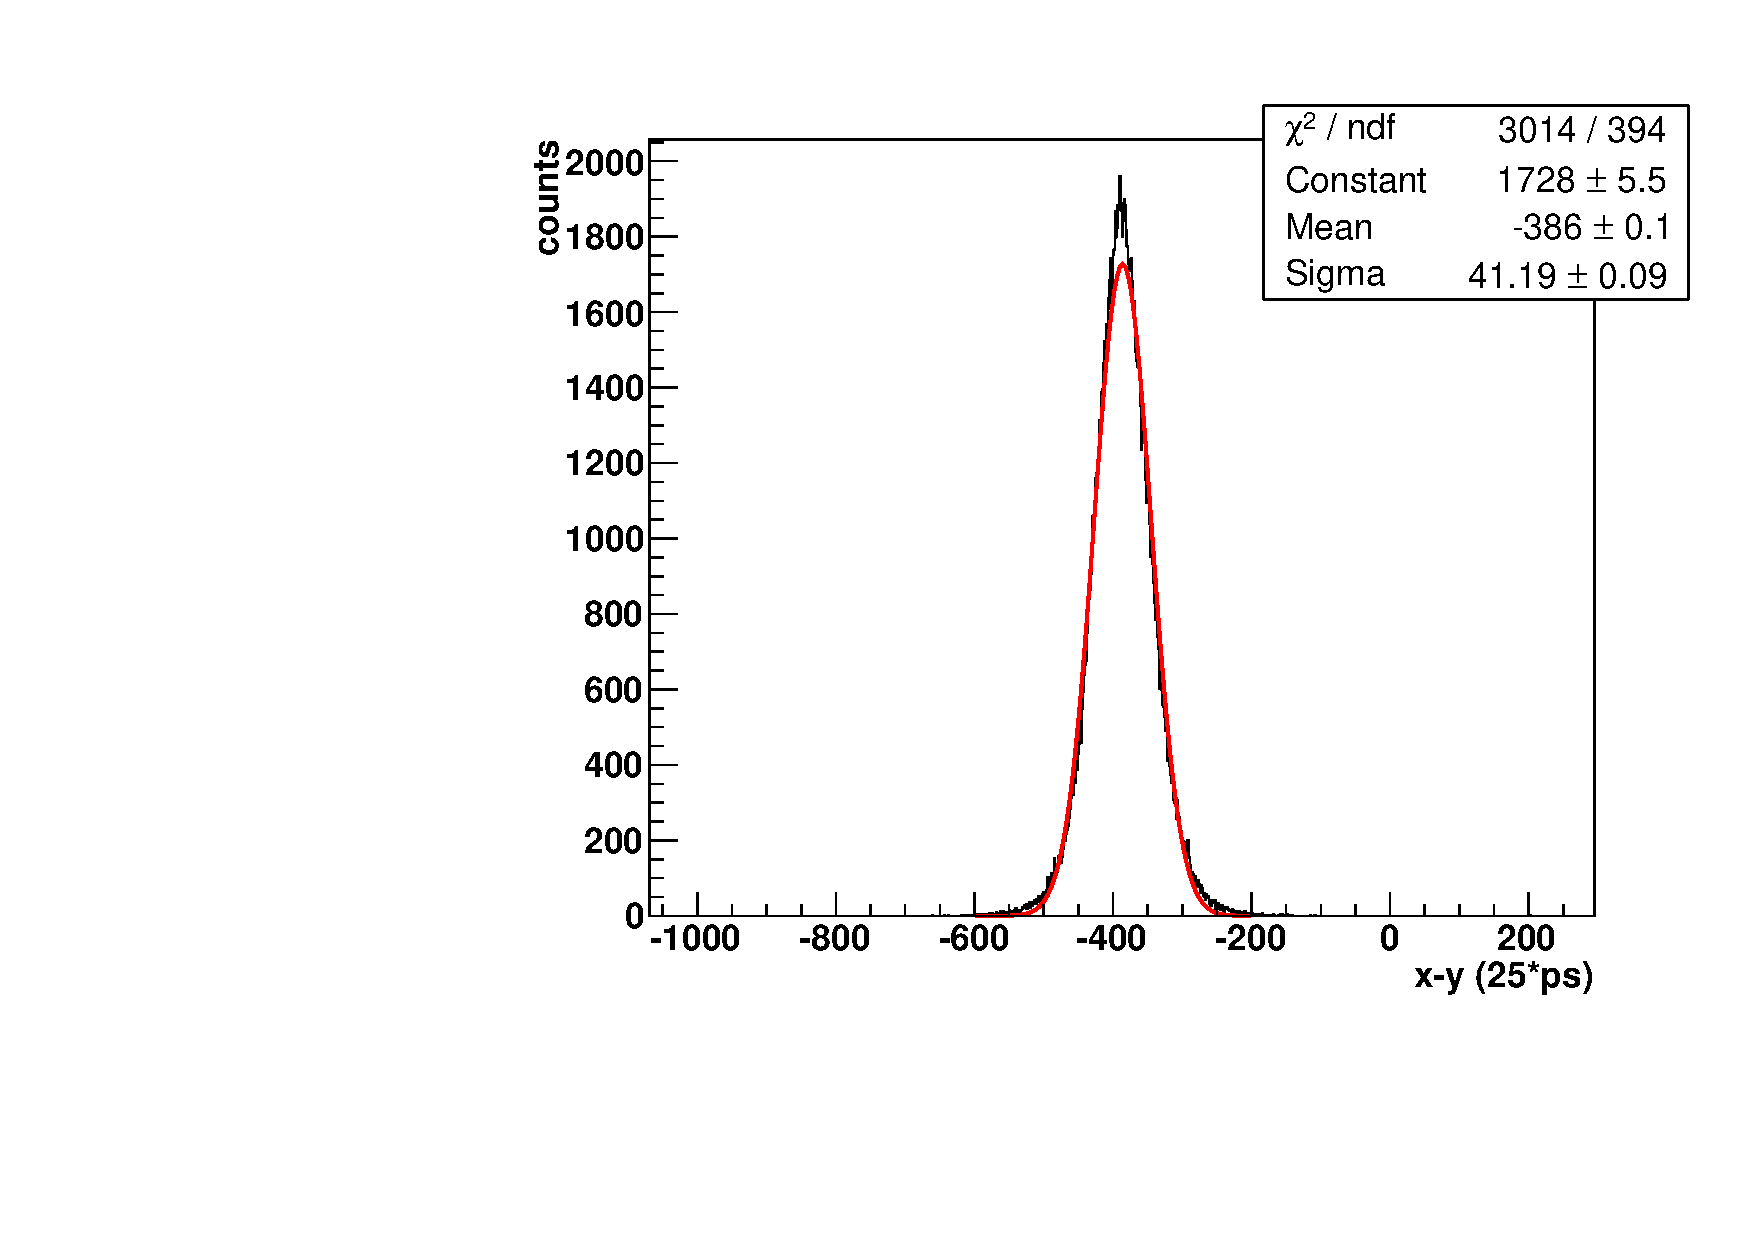
\includegraphics[width=3in]{gleb/fig_gleb_time_walk/vert_cut_fit.pdf}
\caption{$x-y$ distribution, where $x = (TDC1-TDC2)/2$ and $y = (TDC11-TDC12)/2$. Mean value of gaussian fit determine position of red line on Fig.~\ref{fig:vert_cut}. \label{fig:diff_between_diff}}
\end{center}
\end{figure}
Time-walk is an instrumental pulse height dependent shift in the measured time using a leading edge discriminator~\cite{Leo:1987kd}. This time difference is due to the finite rise time of the analog pulse reaching the threshold relative to a reference time. This effect can be minimized in hardware by using constant-fraction discriminators, or by making software corrections to the times using leading-edge discriminators. Since leading-edge discriminator is used one-parameter ($\lambda_i$) time-walk correction is applied to each PMT, where $i$ corresponds to the PMT number.  
In the experemental setup reference time is given by PMT number five, which is attached to the left side of the bar number three. This PMT determines the relative timing of all the other signals.
Accordingly, a single relative time depends on two parameters ($\lambda_i$ and $\lambda_{ref}$) as in Eq.~\ref{eq:t_corr}.
In equation~\ref{eq:t_corr} the second term in each parenthesis is introduced in order to take into account signal rise time.

\begin{equation}
t_{corrected} = \left( TDC_i - \frac{\lambda_i}{\sqrt{ADC_i}} \right) - \left( TDC_{ref} - \frac{\lambda_{ref}}{\sqrt{ADC_{ref}}} \right)
\label{eq:t_corr}
\end{equation}

For each ionizing particle
path $t_{corrected}$ is ideally fixed, so the spreading $\sigma$ of the Gauss fit of the $t_{corrected}$ distribution 
 on a specifed path must be minimized with the two-parameter correction function. For that purposes  each parameter $\lambda$  is varied within the range from -2 to 6, where the spreading of the $t_{corrected}$ distributions is minimal, and plotted as a color code on two dimensionals histograms (see Fig.~\ref{fig:tw_param}). On Fig.~\ref{fig:tw_param} $\lambda_5$ versus $\lambda_i$ is plotted for each PMT except PMT number six since signals from the PMTs five and six are correlated, because they are connected to the same bar. That is why to determine $\lambda_6$  $\lambda_7$ versus $\lambda_6$ is plotted. 






\begin{figure}[]
\begin{center}
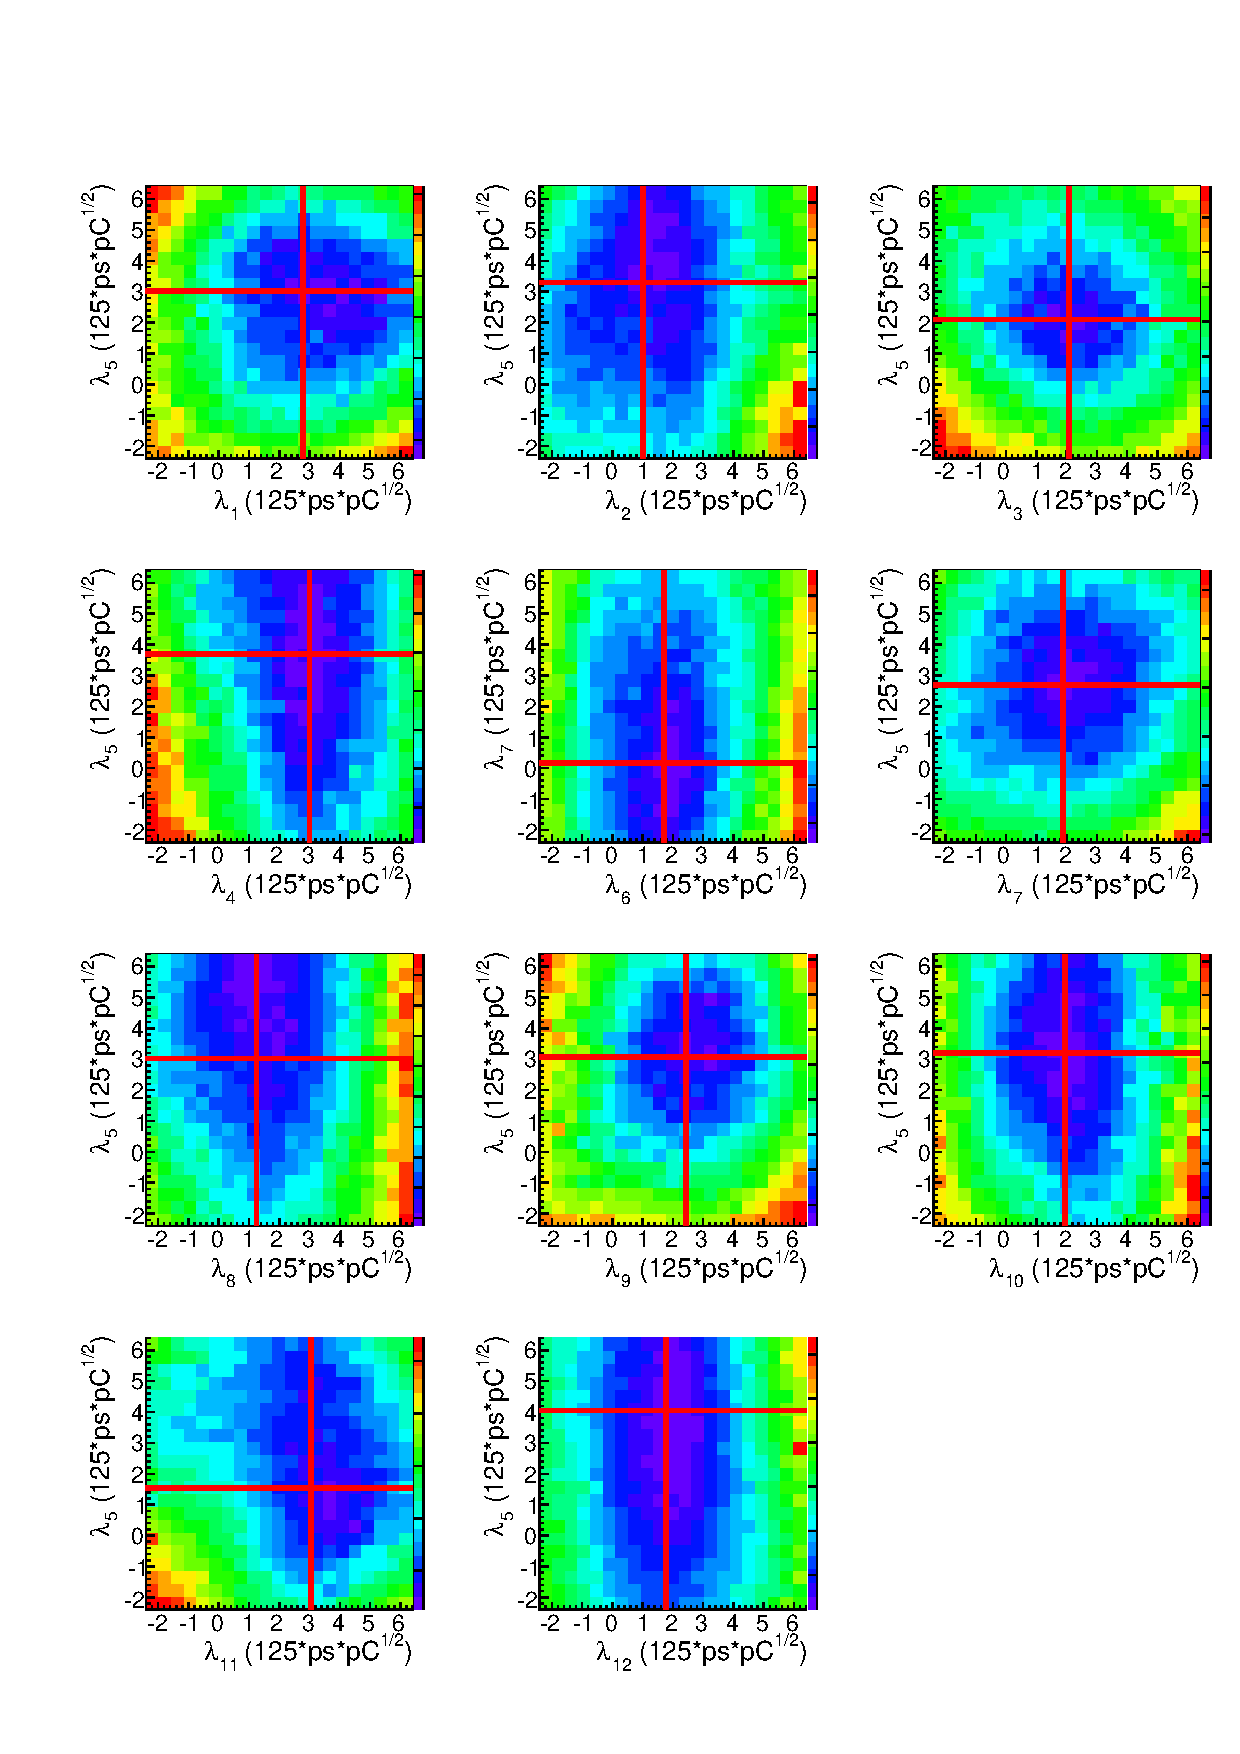
\includegraphics[width=5in]{gleb/fig_gleb_time_walk/tw_param.pdf}
\caption{Two dimensional distributions used to determine time-walk parameters. Coordinate axes correspond to time-walk parameters $\lambda_{i}$ varied from -2 to 6 each. Color code represents spreading of the $t_{corrected}$ distributions (see Eq.~\ref{eq:t_corr}). \label{fig:tw_param}}
\end{center}
\end{figure}

In order to determine the position of the minimum each distribution from Fig.~\ref{fig:tw_param} is fitted by parabolic function. The intersections of red lines show positions of obtained minima. The $x$-coordinate of each minima gives value of $\lambda$ parameters for all PMTs, except PMT five. Since almost all distributions have $\lambda_5$ as $y$-axis, $\lambda_5$ is determined as average value of $y$-coordinates of the minuma for these distributions.


\begin{figure}[]
\begin{center}
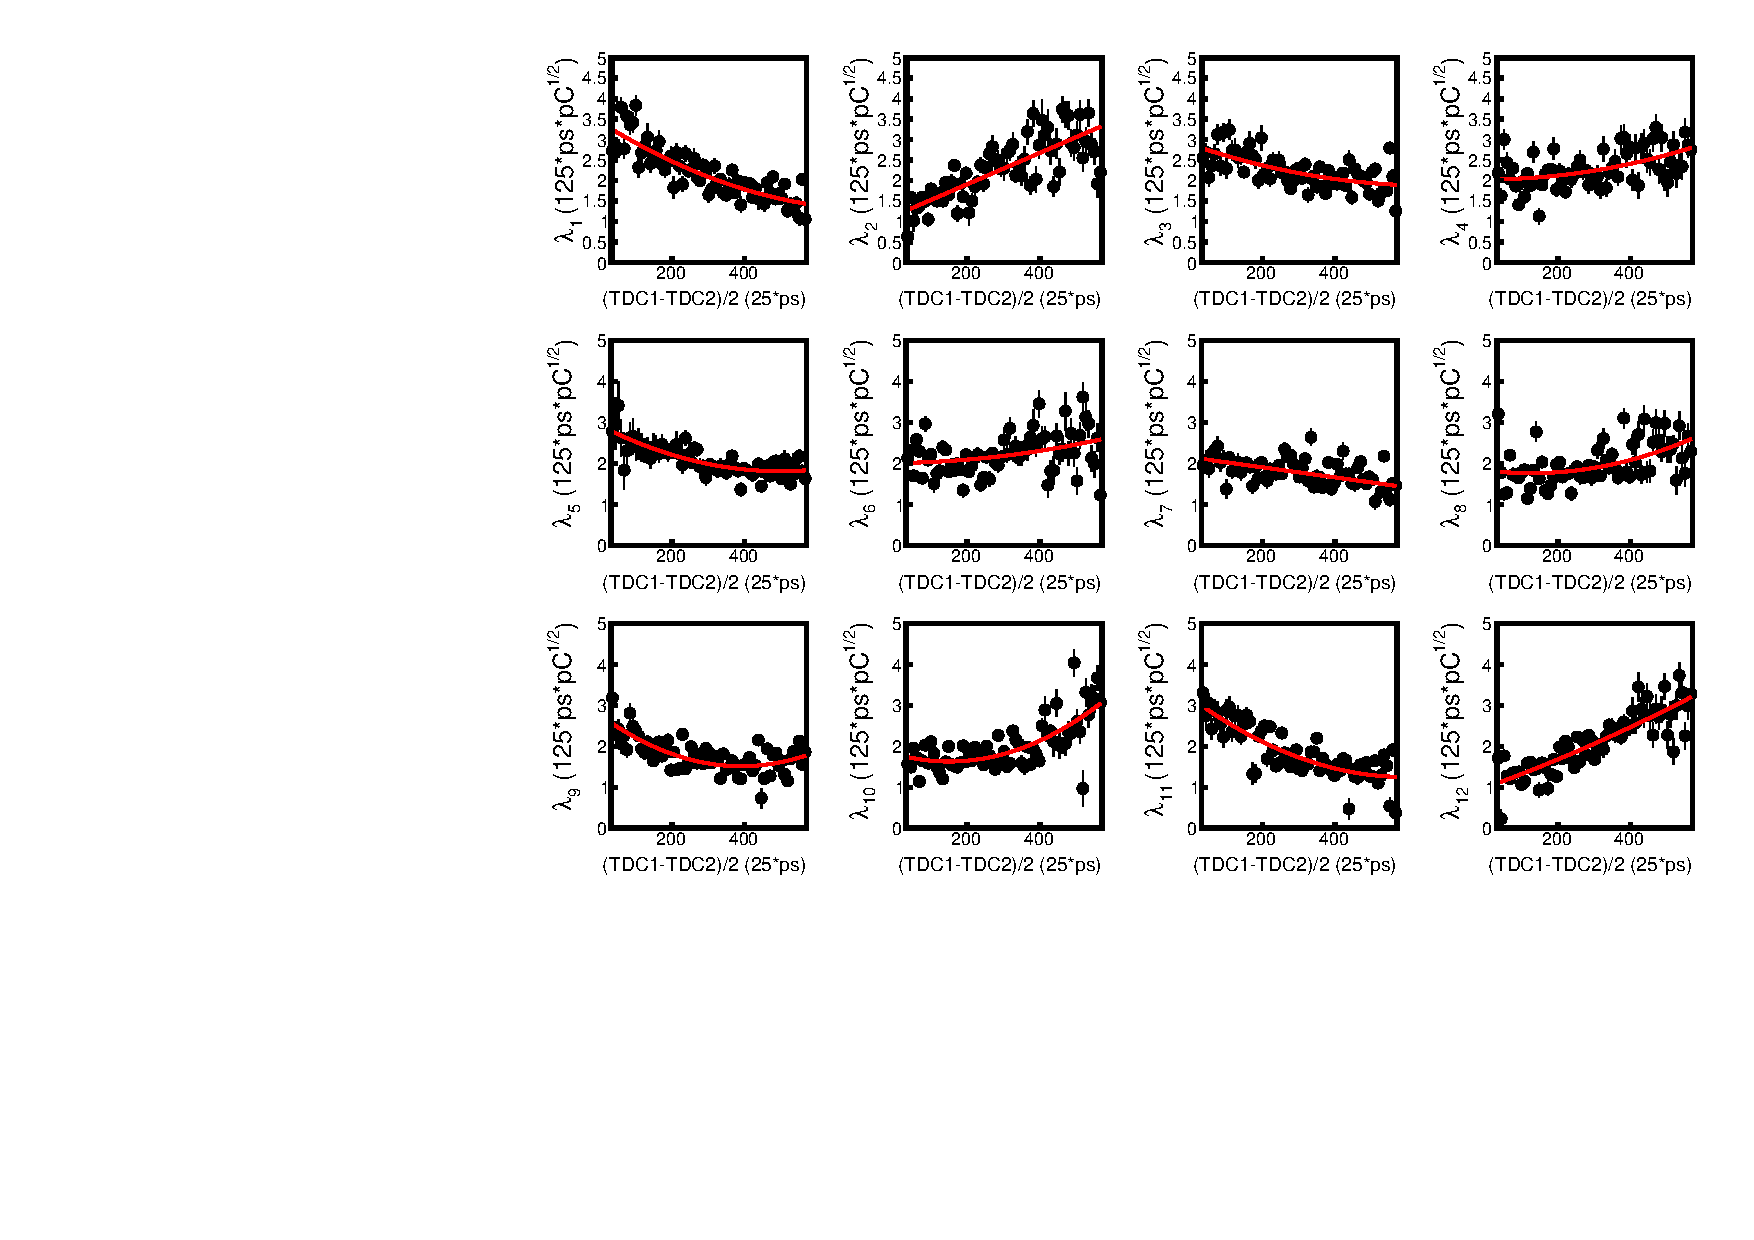
\includegraphics[width=5in]{gleb/fig_gleb_time_walk/tw_params_1d.pdf}
\caption{Time-walk parameters as function of the half of the TDC differences for the bars 200 cm long from the set number 30. Curves represent second order polynomial fit. \label{fig:tw_param_1d}}
\end{center}
\end{figure}

The procedure described above is applied for each bin from Fig.~\ref{fig:vert_cut}. On Fig.~\ref{fig:tw_param_1d}  all extracted $\lambda$ parameters are plotted as a function of TDC differences divided by two that correspond to the length of the scintillator bar. $\lambda$-distribution for each PMT is fitted by second order polynomial. Finally for calculations of time-walk corrected times $\lambda$-parameters as smooth function of bar length is used.
 





\section{III.E. Photomultiplier tubes (PMTs)}

\subsection{Different PMTs time resolutions}
\textit{My assumptions in writing this section}
\begin{enumerate}
	\item \textit{Our chosen PMT(R9779) was compared with panel-1a PMT(EMI9954A)}
	\item \textit {Details of relevant differences of the tech-specs of the two PMTs and therefore the expected superiority of R9779 over EMI9954A will be listed elsewhere; here we will only give empirical proof}
\end{enumerate}

The selected Hamamatusu's R9779 PMTs for panel-1b were compared with Electron Tubes EMI 9954A in the 3-bar setup (\textit{I am assuming that the 3-bar setup will either already be defined or referred to in another publication, so as to not go into details, but simply for the reader to trust that it is our way to extract time-resolution, though, it is NOT directly the time-resolution of the PMT, but of the entire counter; this is important to keep in mind, since for the old TOF system, PMT resolutions were directly compared using lasers; details of this method are in old CLAS-SC NIM paper.})

\textit{Should I mention here that for EMI PMT tests, the contribution of the LFIO module was removed?}

Below is the figure that shows the superiority of the R9779:
\begin{figure}[th]
	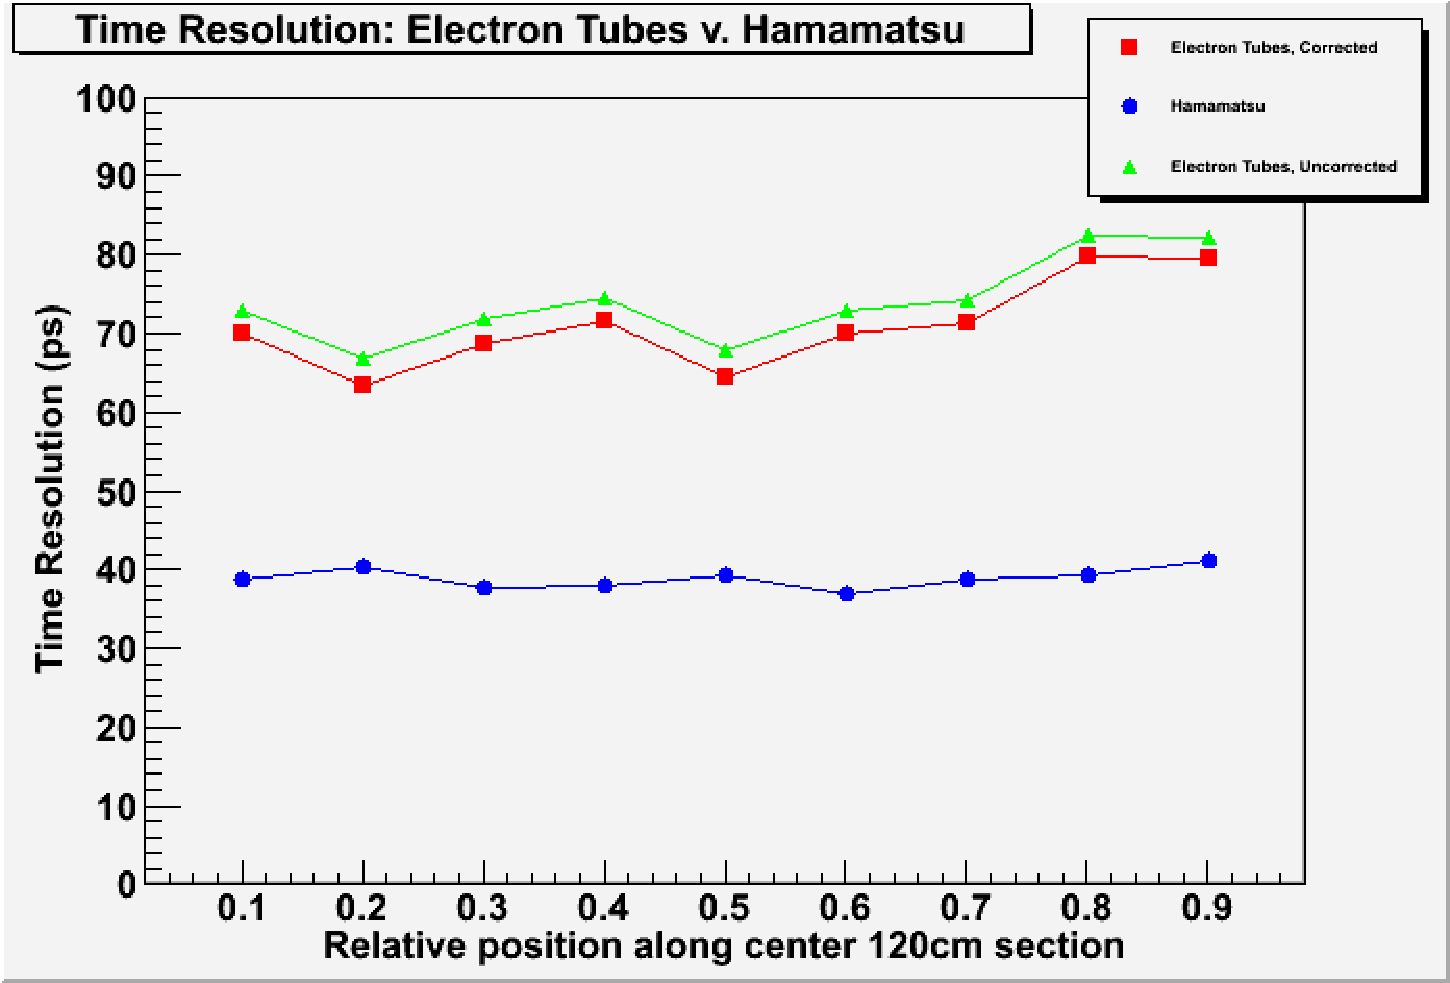
\includegraphics[width=10cm, height=5cm]{arjun/fig_arjun_pmt_resolution/PMTcomparison.pdf}
\end{figure}

\subsection{... threshold dependence}
We also compared various threshold (\textit{Define "threshold"}) levels for the signals from the PMT and see if it had any affect on the time resolution. The threshold levels tried were:50mV, 75mV, 150mV, 300mV, and 600mV.

Following is a figure that demonstrates varying the threshold did not affect the time resolution.
\begin{figure}[th]
	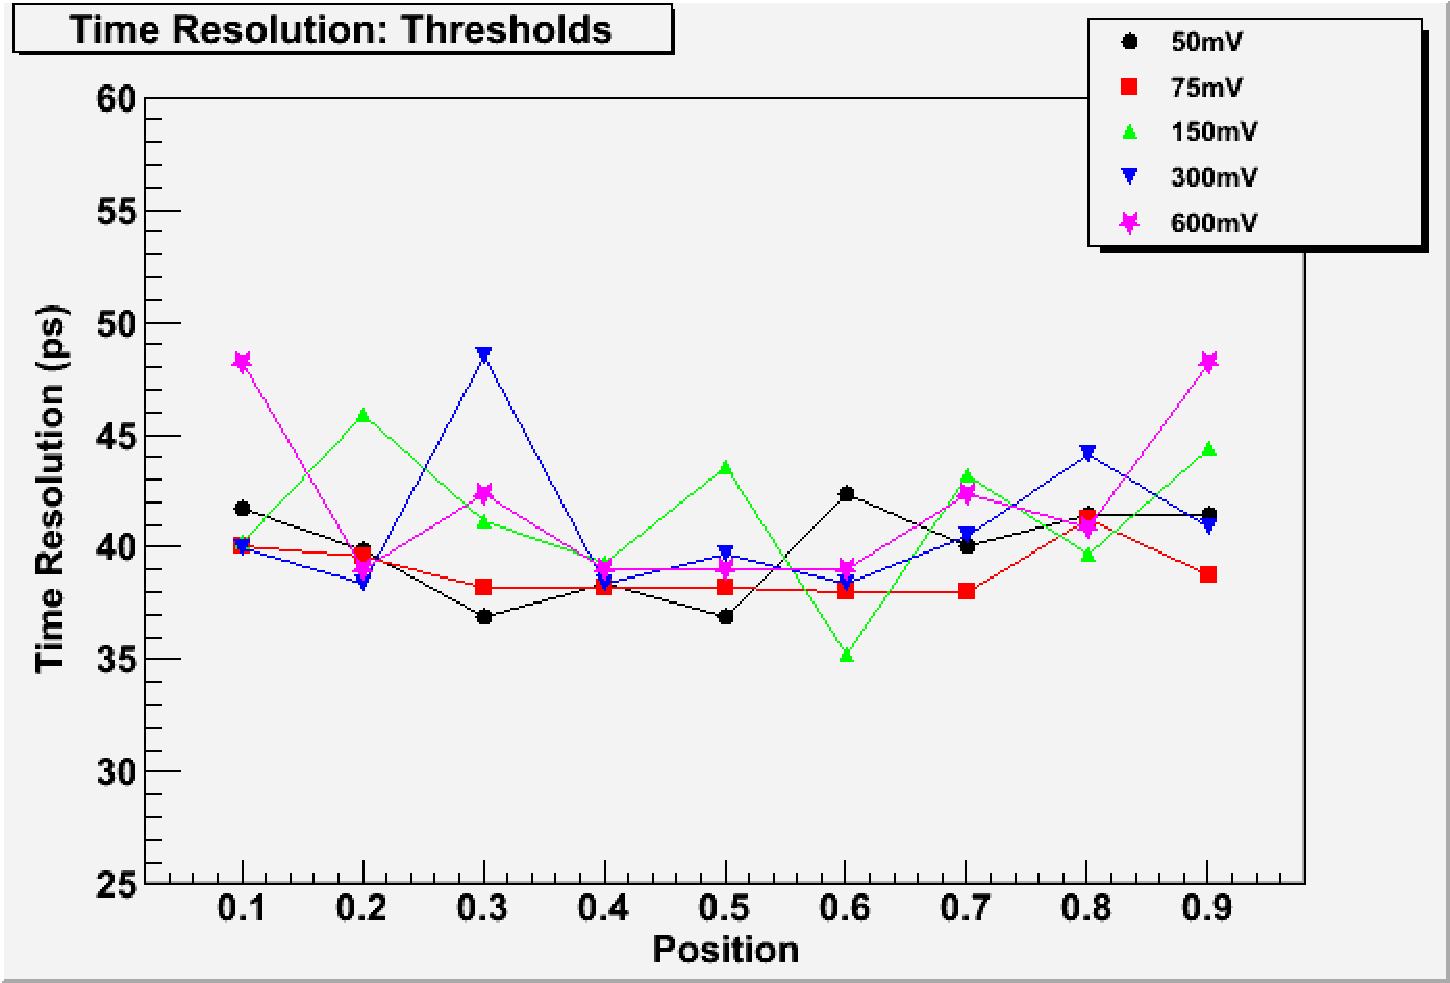
\includegraphics[width=10cm, height=5cm]{arjun/fig_arjun_threshold/ThresholdsTimeRes.pdf}
\end{figure}

\section{III.G. Magnetic shielding of the PMTs}
The photomultipliers that are attached to the FTOF scintillators will be exposed to the combined stray magnetic fields from the CLAS12 solenoid and torus magnets. It is therefore important to study the effect of the magnetic field strength on the anode signal of a PMT and ultimately on the time resolution of the FTOF detector system. In the experimental test setup, a PMT was set on a flat, non-magnetic base in between a pair of Helmholtz coils and the anode signal of the PMT was digitized and processed by a DAQ system . This arrangement is shown in Fig. 1.

\begin{figure*}[ht]
  \includegraphics[width=2.5in]{arjun/fig_arjun_magnetic_shielding/placeholder.pdf} 
  \caption{PMT B field test setup}
  \label{fig1}
\end{figure*}

Due to the dynode-array geometry of the PMT and the electrodynamic processes which finally contribute to the signal formation, the studies need to be performed in dependence of the orientation of the PMT relative to the magnetic field. Given the axial Helmholtz magnetic field, the orientation of a PMT in it can be described by two rotational degree of freedoms; their axes are illustrated in Fig. 2 and defined by the PMT's axis of cylindrical symmetry, $\hat{z}$ and the radial axis perpendicular to $\hat{z}$ and horizontal to the flat base supporting the PMT, $\hat{\rho}$.

In the axial Helmholtz magnetic field, a PMT can be rotated around $\hat{\rho}$ until $\hat{z}$ is aligned transversely (T) or longitudinally (L) with the field direction. These are the two orientations in which a PMT is observed to have the two strongest and in a sense, independent responses; any other orientation is dominated by a superposition of the two responses. These two orientations are illustrated in Fig. 2.

\begin{figure*}[ht]
  \includegraphics[width=2.5in]{arjun/fig_arjun_magnetic_shielding/placeholder.pdf} 
  \caption{Tranverse and longitudnal orientations of PMT in axial B field}
  \label{fig2}
\end{figure*}

The additional change in the signal response of a PMT when it was rotated around $\hat{z}$ was also studied, primarily when it is already aligned in the transverse orientation (minimal to no effect due to rotations around $\hat{z}$ is observed in the longitudinal orientation) \cite{Steinman} However, after implementing the final shielding configuration (see Sec. 2.2), the PMT response no longer depends on the rotational degree of freedom around $\hat{z}$.

It is worth mentioning here that the magnetic field primarily affects the signal amplitude, while the signal shape and smoothness, which have a far larger impact on the time resolution, are mostly unaffected \cite{Steinman}. However, the loss of signal amplitude does affect the extracted time resolution, but only when the reduction reaches levels at which the Time-walk corrections become less efficient. Therefore, the signal reduction level was used as the parameter to quantify the response of a PMT in a magnetic field and its affect on the time resolution. 

Even though it was established that when the signal amplitude is reduced by 10\% in the longitudinal and the transverse orientations there is no change in the time resolution - measured to be $41\;ps$ and $38\;ps$, respectively ($39\;ps$ with no magnetic field) \cite{Steinman} -  the final design of the magnetic shielding (Sec. 2.2) is such that up to magnetic field strengths higher than those expected in CLAS12, the signal amplitude shows no reduction; the maximum stray field strength that the panel-1b PMTs are going to be exposed to is expected to be 22G at counters placed at the largest angular extent of the FTOF12 detector system, of which 2/3 (15G) will be in the axial direction \cite{CLAS12FTOFstudies} and the tests at USC were done with magnetic fields up to 30G, wholly directed in either the transverse or longitudinal directions.

\subsection{Initial design considerations}
The PMT assemblies R9779-20MOD are already manufactured with a layer of mu-metal coating. It can be seen from Tab. 1 that in the transverse orientation, compared to a PMT without any mu-metal coating, the inbuilt mu-metal shielding preserves the signal amplitude to much higher levels of magnetic fields.

\begin{table}[H]
	\begin{center}
		\begin{tabular}{|c|c|l|}
			\hline
	 		& no mu-metal & with mu-metal \\
			\hline
 			10G-L & 10\% & 10\% \\
 			10G-T & 100\% & 0\% \\ 
 			\hline
 			15G-L & XX\% & XX\% \\
 			15G-T & 100\% & 0\% \\
 			\hline
 			15G-L & YY\% & YY\% \\
 			15G-T & 100\% & 0\% \\
 			\hline
 			20G-L & ZZ\% & ZZ\% \\
 			20G-T & 100\% & 10\% \\
 			\hline
 			25G-L & AA\% & AA\% \\
 			25G-T & 100\% & XX\% \\
 			\hline
 			30G-L & BB\% & BB\% \\
 			30G-T & 100\% & BB\% \\
 			\hline
		\end{tabular}
	\end{center}
	\caption{Reduction of PMT anode signal in various test configurations}
\end{table}


However, even with the inbuilt mu-metal shielding, there is a rapid deterioration of the signal past 10G-L and XXG-T and this led to considering further shielding methods.

\subsubsection{External shielding}
In order to provide additional shielding, a rectangular external mu-metal shielding, with each side of thickness $2\;mm$, was designed. Tab. 2 shows that within this external shielding, in the transverse orientation, the signal amplitude is preserved up to $30\;G$. However, this provided no additional protection to PMT in the longitudnal orientation.

\begin{table}[H]
	\begin{center}
		\begin{tabular}{|c|c|}
			\hline
	 		& external mu-metal shielding \\
			\hline
 			10G-L & 10\% \\
 			10G-T & 0\% \\ 
 			\hline
 			15G-L & XX\% \\
 			15G-T & 0\% \\
 			\hline
 			15G-L & YY\% \\
 			15G-T & 0\% \\
 			\hline
 			20G-L & ZZ\% \\
 			20G-T & 0\% \\
 			\hline
 			25G-L & AA\% \\
 			25G-T & 0\% \\
 			\hline
 			30G-L & BB\% \\
 			30G-T & BB\% \\
 			\hline
		\end{tabular}
	\end{center}
	\caption{Signal reduction of PMT's anode signal in presence of external mu-metal shielding. It is observed that PMT signal's reduction is unchanged in the longitudinal orientation, but the signal is preserved to $30\;G)$ in the transverse orientation}
\end{table}

\subsection{Final implementation of shielding with overhang}
To also preserve the signal amplitude in the longitudinal orientation, it was decided that in the final implementation, the external shielding would extend a few centimeters beyond the front face of the PMT ($\defeq$ overhang). This requires shaving two edges of the scintillator bars by a few millimeters. Tab. 4 shows the results of testing the signal reduction at various overhang positions of the external shielding. The overhang position of $4\;cm(1.5\;in)$ is sufficient to preserve the signal up to $30\;G$ in the longitudinal orientation.

\begin{table}[H]
	\begin{center}
		\begin{tabular}{|c|c|c|c|c|c|}
			\hline
	 		& $0\;cm$-overhang & $1\;cm$-overhang & $2\;cm$-overhang & $3\;cm$-overhang & $4\;cm$-overhang \\
			\hline
 			10G-L & & & & & \\
 			10G-T & & & & & \\ 
 			\hline
 			15G-L & & & & & \\
 			15G-T & & & & & \\
 			\hline
 			15G-L & & & & & \\
 			15G-T & & & & & \\
 			\hline
 			20G-L & & & & & \\
 			20G-T & & & & & \\
 			\hline
 			25G-L & & & & & \\
 			25G-T & & & & &\\
 			\hline
 			30G-L & & & & & \\
 			30G-T & & & & & \\
 			\hline
		\end{tabular}
	\end{center}
	\caption{Signal reduction of PMT's anode signal in presence of external mu-metal shielding at various overhang positions. It is observed that at the overhang position of $4\;cm$ the signal is preserved up to magnetic field strength of $30\;G$ in both the transverse and longitudinal orientations}
\end{table}

\section{Establishing an upper limit on the level of tolerable magnetic field} In the final design and implementation of the magnetic shielding, the tests show that there is going to be no reduction in signal amplitude in fields up to $30\;G$ in the transverse and longitudinal orientation. This is already beyond the maximum fields to which the PMTs will be exposed to according to the CLAS12 design requirements \cite{CLAS12FTOFstudies}. However, tests were run to note signal reduction levels as the magnetic field strength was increasted beyond $30\;G$ in each of the orientations and the point at which the signal amplitude reduced by 10\% in each of the orientations, transverse and longitudinal, was noted. Since up to such reduction levels, the time resolution is unaffected, the noted field strength serves as the conservative upper limit of the magnetic field at which the time resolution remains unaffected. Tab. 4 shows the results of such tests which establishes the conservative upper limit at $XX\;G$ and $YY\;G$ in the transverse and longitudinal orientations, respectively.

\begin{table}[H]
	\begin{center}
		\begin{tabular}{|c|c|}
			\hline
			30G-L &  \\
 			30G-T &  \\ 
 			\hline
 			35G-L &  \\
 			35G-T &  \\
 			\hline
 			40G-L &  \\
 			40G-T &  \\
 			\hline
 			45G-L & \\
 			45G-T &  \\
 			\hline
 			50G-L &  \\
 			50G-T &  \\
 			\hline
 		\end{tabular}
	\end{center}
	\caption{Signal reduction of PMT's anode signal beyond the design consideration of $30\;G$}
\end{table}

\subsection{Results and Conclusions}
With the finally designed and implemented shielding, the time resolution of the panel-1b FTOF counters remains unaffected by the presence of fringe magnetic fields in CLAS12 up to a field level of at least $XX\;G$ and $YY\;G$ in the transverse and longitudinal orientations, respectively. This exceeds the maximum field of $22\;G$ (of which 2/3 will be in longitudinal direction) to which the panel-1b PMTs are expected to be exposed to.

\section{G Scintillator Geometry and Light guides }

When a particle is passing through the scintillator, it ionizes the material and generates scintillation light. These photons travel via different paths through the scintillator, can be absorbed and reflected, then get converted by the photocathode of the Photomultiplier Tube (PMT), generating a photoelectron current. This current is amplified by the PMT and becomes a measurable electronic pulse (see Fig: (pulse) in time walk or shielding section). Finally, the pulse passes through the electronic system and is read out by the computer. All these various processes affect the total time resolution $\sigma_{ToF}$. Therefore, it is convenient to parameterize the length averaged time resolution $\overline{\sigma_{ToF}}$ by
\begin{equation}
\overline{\sigma_{ToF}}=\sqrt{\sigma_{0}^{2}+\frac{\sigma_{1}^{2}+(\sigma_{p}\frac{L}{2})^{2}}{N_{pe}exp(-\frac{L}{2\lambda})}} .
\label{eq:1}
\end{equation}
The parameters in this equation quantify the characteristics of the detector geometry and components, here, $\sigma_{0}$ is the intrinsic resolution of the electronics and other processes that are independent of the light intensity, $\sigma_{1}$ models the jitter in the combined single-photoelectron response of the scintillator and PMT, and $\sigma_{P}$ accounts for path length variations in the light collection. The distance from the source to the PMT, which for $\overline{\sigma_{ToF}}$ is taken to be half the length of the counter($\frac{L}{2}$), and $\lambda$ is the attenuation length of the scintillator. $N_{pe}$ is the average number of the photoelectrons seen by the PMT of a counter with an infinitely long attenuation length. The statistical behavior of $\sigma_{1}$ and $\sigma_{p}$ is encoded by scaling the single-photoelectron responses by $\sqrt{N_{pe}}$.

The geometry of the individual FToF12 detectors has to be optimized, since it influences the time resolution. Figure~\ref{f:averagesigma} uses equation~\ref{eq:1} to show how the length, width, and thickness of detectors typical for the CLAS12 design requirement affect the time resolution, where he parameters of the time resolution for the existing panel 1a counters are given in Ref ~\cite{smith1999time}. The design requirement for panel 1b is to achieve a combined time resolution for panel 1a and 1b of $80\;ps$ for all scintillator up to $4\;cm$ length.
\begin{figure}[ht!]
\centerline{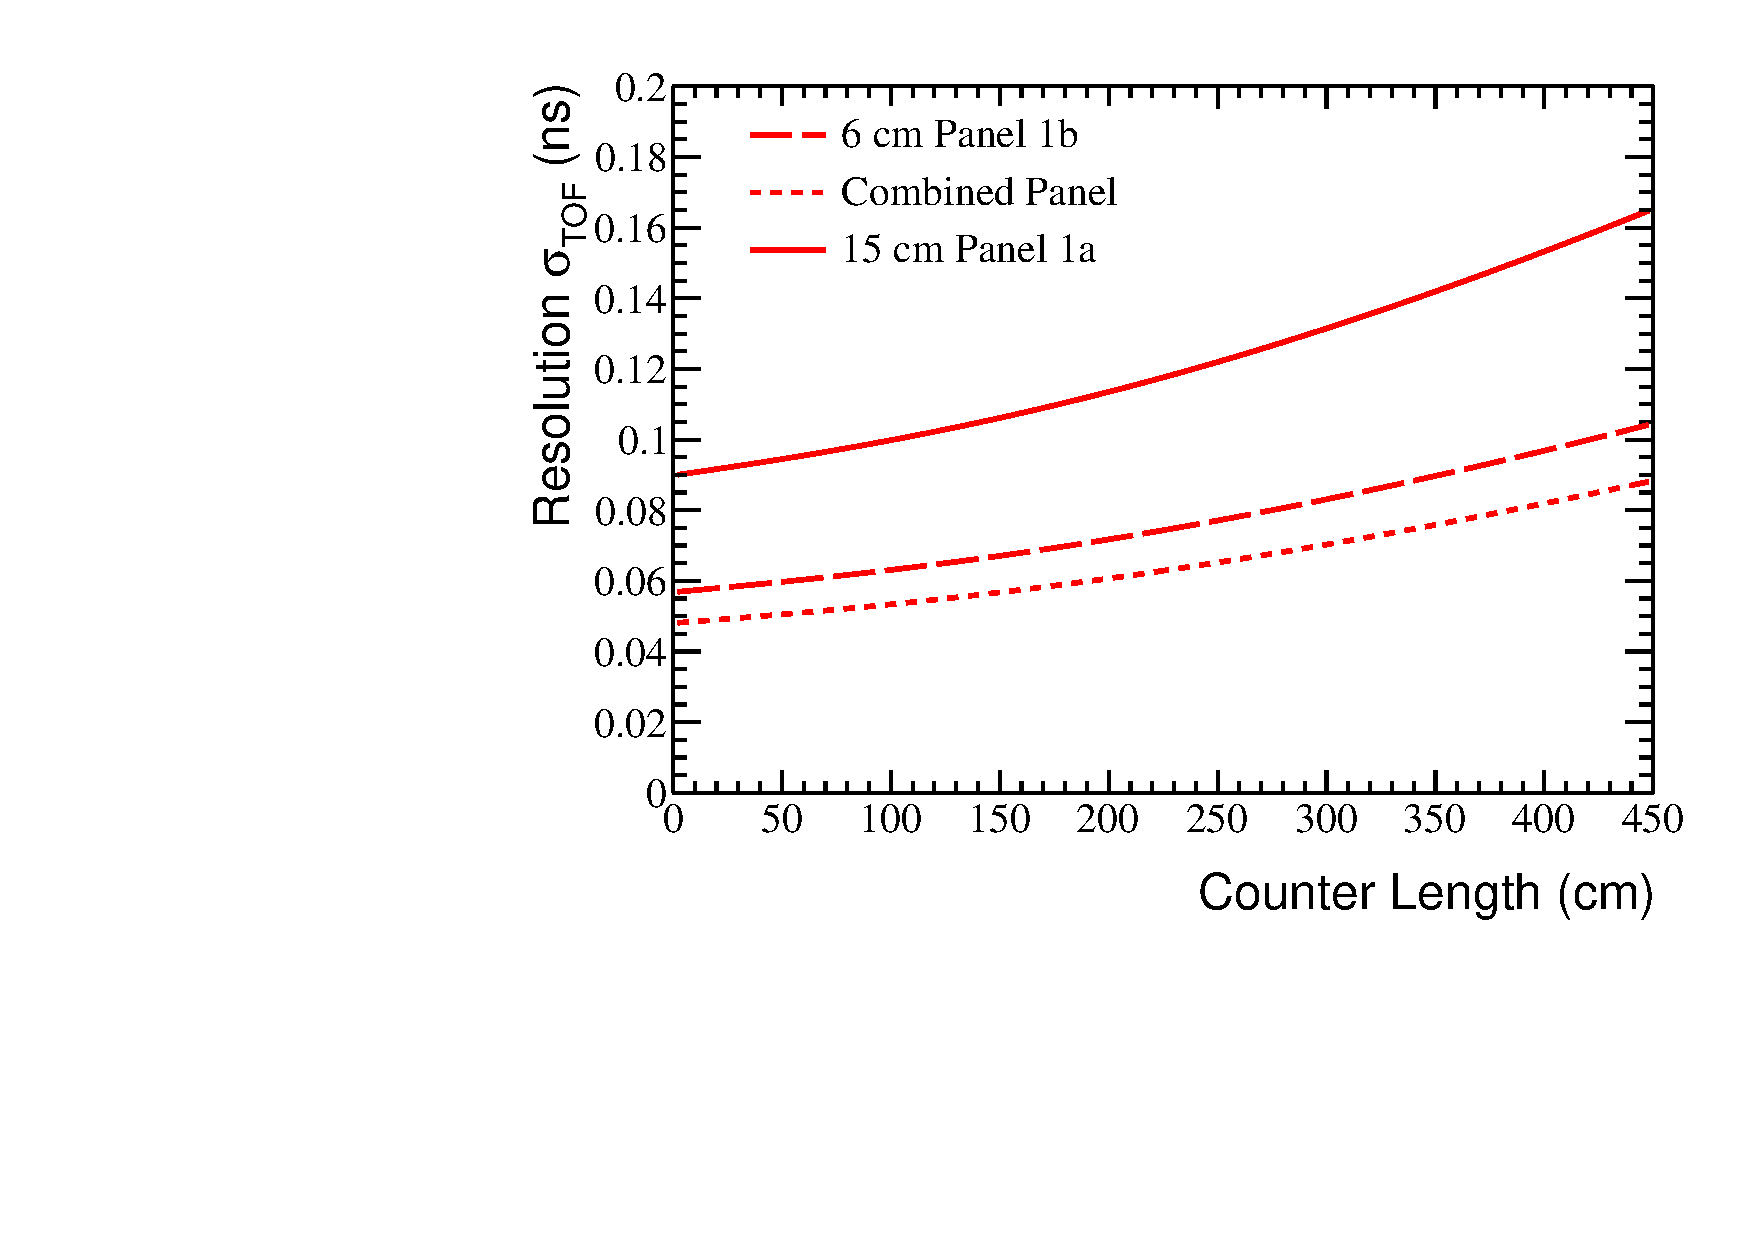
\includegraphics[width=13cm,height=10cm]{ye/fig_ye_geometry/DR.pdf}}
\caption{Solid line, the measured and parameterized average standard deviation $\overline{\sigma_{ToF}}$ time resolution of the existing panel-1a counters ($15\;cm$ wide, $5\;cm$ thick) fit with an assumed intrinsic electronic resolution of 40 ps ~\cite{smith1999time}. Scaling the parametrization by $\sqrt{\frac{2}{5}}$ leads to the  Long dashed line representing the new panel-1b counters (6cm wide, 6cm thick) and short dashed line the combined panel-1a and panel-1b counters time resolution.}
\label{f:averagesigma}
\end{figure}

The most obvious improvement of the time resolution of a detector can be accommodated by increasing the photon statics $N _{pe}$, since the time resolution is proportional to $\sqrt{N_{pe}}$. The number of photons reaching the photocathode scales with the ratio of PMT entrance over exit window areas and the thickness of the scintillator. Given the same PMT diameters, changing the geometry (width $\times$ thickness) from $15\times5\;cm^{2}$ to $6\times6\;cm^{2}$ leads to an increase of $N _{pe}$ by $\frac{15}{6}$. The loss of light from a scintillator can occur in two basic ways; one is the escape of light at the scintillator surface. The simplest and most common practice is to redirect escaping light by total reflection. To maximize the internal reflection, any reflecting film should be loosely wrapped with an air gap to the scintillator, which is described in Sec.I. The other one is through absorption by the scintillation material itself, which is related to the attenuation length consideration described in Set.H.

In contrast to the total reflection requirement discussed above, for the coupling between the scintillator and the PMT, the refraction index change should be minimized to maximize light transmission. Additionally, the PMT is often coupled to the scintillator by a light guide to match the geometry of scintillator to the circular entrance surface of PMT, as in the case of the FToF panel 1a detectors. In the prototyping phase, simulations done to optimized the shape and length of light guides coupling the square exit window of the scintillator to the circular PMT entrance window were carried out. Under best conditions a monotonically increasing a mount of light is lost up to a light guide length of $6\;cm$, which would already liit the over all acceptance of the CLAS12 detectors. Hence the simulation shows that the best light transmission is achieved when the PMT is directly attached to the scintillator. The result was experimentally verified by comparing the scintillator without and with 7cm-long light guide. In order to quantify the time resolution with or without light guide, three-bar time resolution measurements described in Sec. III B were utilized to extract the time resolution of the middle bar under both conditions, respectively. Without light guides, the Hamamatsu PMTs were directly mounted to the left and right ends of a $5 \times 5 \times 150\;cm^{3}$ BC408 scintillator. With light guides, the light guides were first wrapped with aluminized mylar and then
attached to both ends of the same $5 \times 5 \times 150\;cm^{3}$ BC408 scintillator, and the same Hamamatsu PMTs were mounted to light guides.
\begin{figure}[ht!]
\centerline{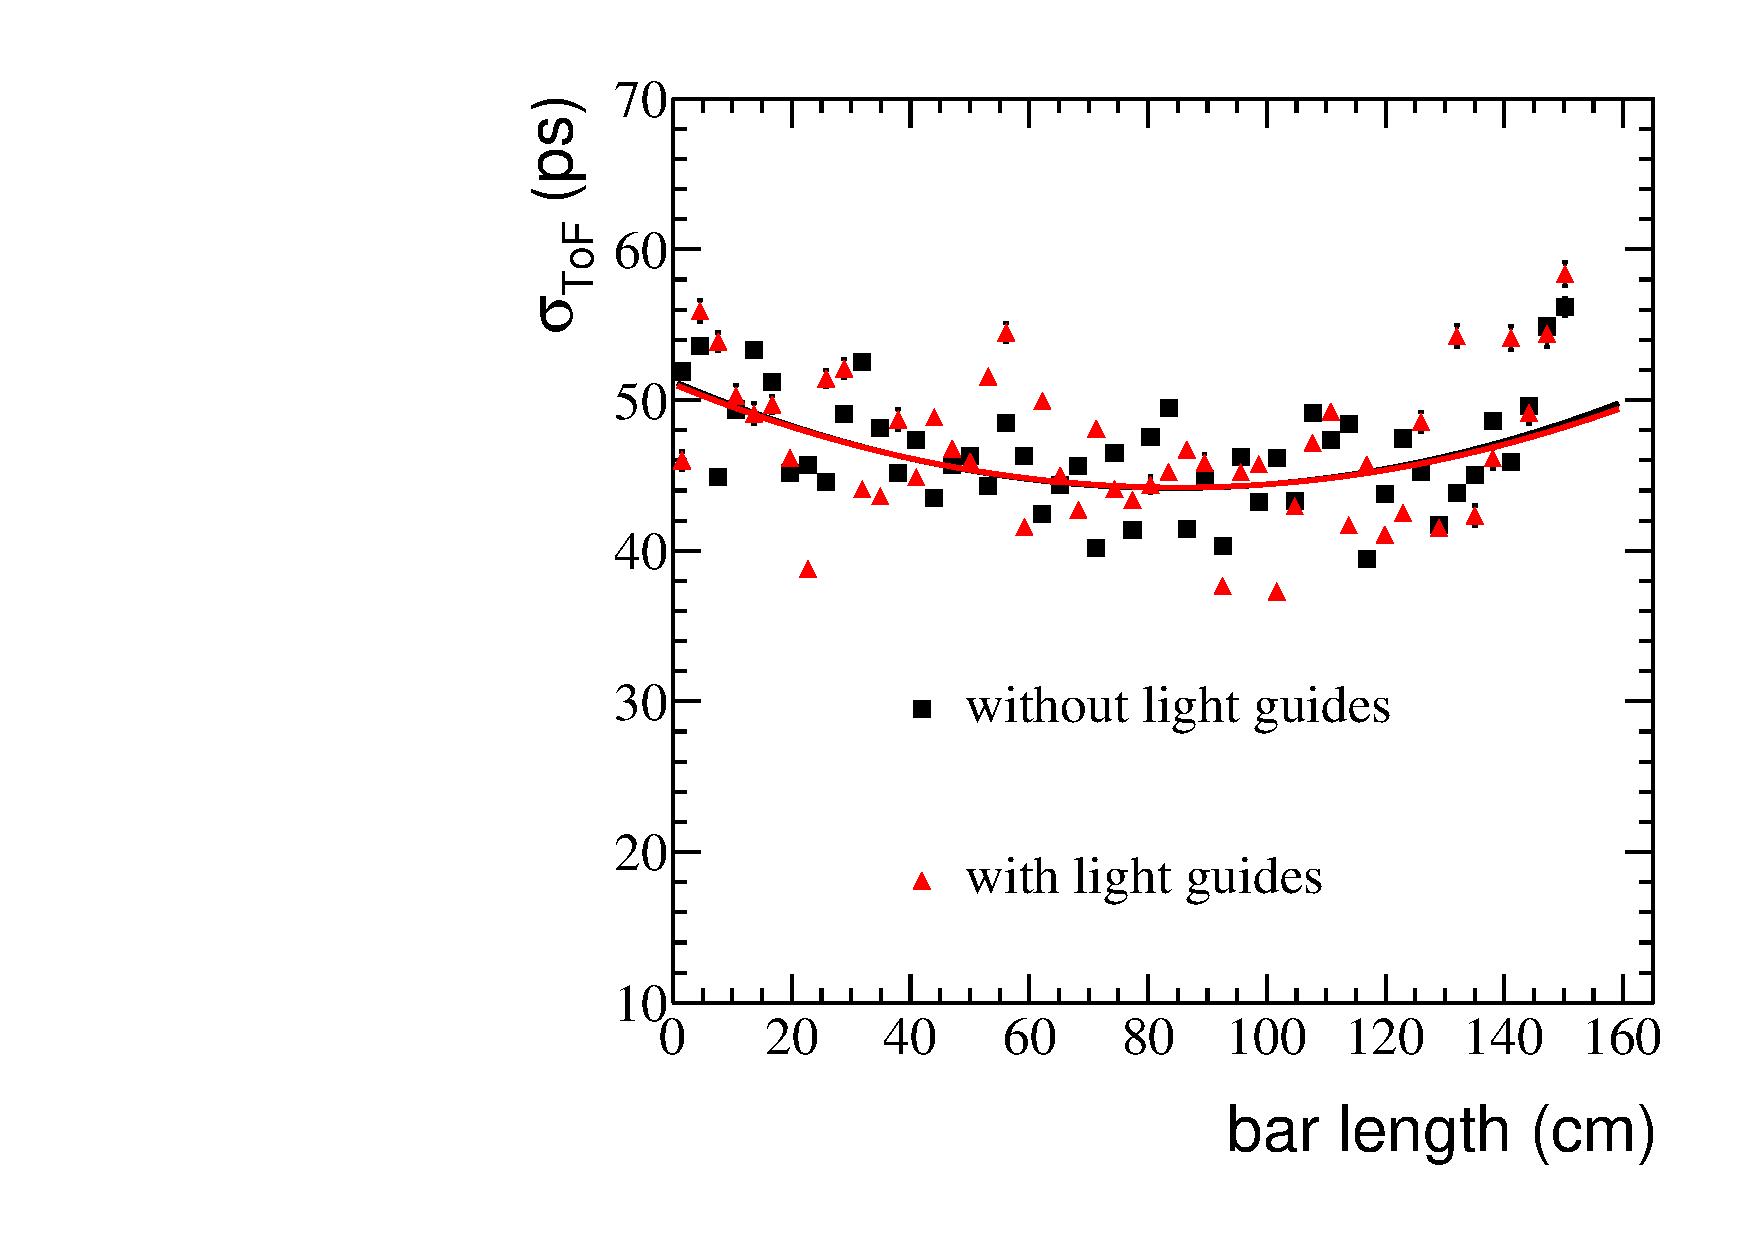
\includegraphics[width=15cm,height=12cm]{ye/fig_ye_geometry/TR_LG.pdf}}
\caption{Black squares, position dependent time resolution of a $5 \times 5 \times 150\;cm^{3}$ BC408 scintillator with and red triangles without light guides. }
\label{f:lightguides}
\end{figure}
Figure~\ref{f:lightguides} shows that the average time resolutions of scintillator with and without light guides are $46.879\;ps$ and $46.519\;ps$, respectively. Even though, the time resolution of scintillator without light guide is a slightly better, the influence of the light guide is still negtigible with in error bars, eliminating the light guides allows for long scintillators covering full fiducial region of CLAS12.

\section{H Scintillator}
Since the time resolution is proportional to $\sqrt{N_{pe}}$, in order to improve the time resolution, the scintillator material for the TOF system must have fast decay times, long attenuation length, and good spectral match to the PMTs. The attenuation length of scintillator can be divided into two parts. One part is called the technical attenuation length (TAL), which is defined as the length reducing the amount light by a factor e and which depends
on the geometry the scintillator and the reflective properties of its surface. The other part is called bulk attenuation length (BAL), which reduces the initial light intensity by a factor $e$ according to the Buger-Lambert Law and which depends on the transparency and the scintillation material. From the design requirement, the counter length of CLAS12 panel 1b detectors varies from $17.27cm$ to $407.9cm$, so it is important to find the right material for all counters. The Table~\ref{table1} shows that scintillator material $EJ200$ and $BC408$ both have longer attenuation length and slower decay time. $EJ204$ and $BC404$ both have shorter attenuation length and faster decay time. The time resolution of these scintillator material for $50$ $cm$-long bars are measured. The comparison results are shown in Fig.~\ref{f:TRmaterial}, there is no big difference between different material.

\begin{table}[h]
\begin{center}
\begin{tabular}{|c|c|}
\hline
Plastic Scintillator &
\multicolumn{1}{|c|}{Decay Time}\\
\hline
EJ200  &     2.1ns (slow)\\
EJ204  &     1.8ns (fast)\\
BC408  &     2.1ns (slow)\\
BC404  &     1.8ns (fast)\\
\hline
\end{tabular}
\caption{Scintillator comparing}
\label{table1}
\end{center}
\end{table}

The parametrization of $\overline{\sigma_{ToF}}$ is used to study the possible improvements in time resolution based on a trade-off between the decay time of the scintillator and the number of photoelectrons arriving at the PMT, which depends on the attenuation length~\cite{smith1999time}. Fig.~\ref{f:tradeoff} shows the expected time resolution plotted as a function. Based on the fast decay time of $BC404$, it is used as shorter bar's material. For longer counters, the existing material $BC408$ with its larger attenuation length is the better choice. In the Fig.~\ref{f:tradeoff} there is a time resolution crossing point around $200$ $cm$. Below it, the counters with $BC404$ material have better time resolution and above it, the $BC408$ counters have better time resolution. From the above information, we decided to use $BC404$ material for the length of counters shorter than $200$ $cm$ and $BC408$ material for the counters longer than $200$ $cm$.

\begin{figure}
\centerline{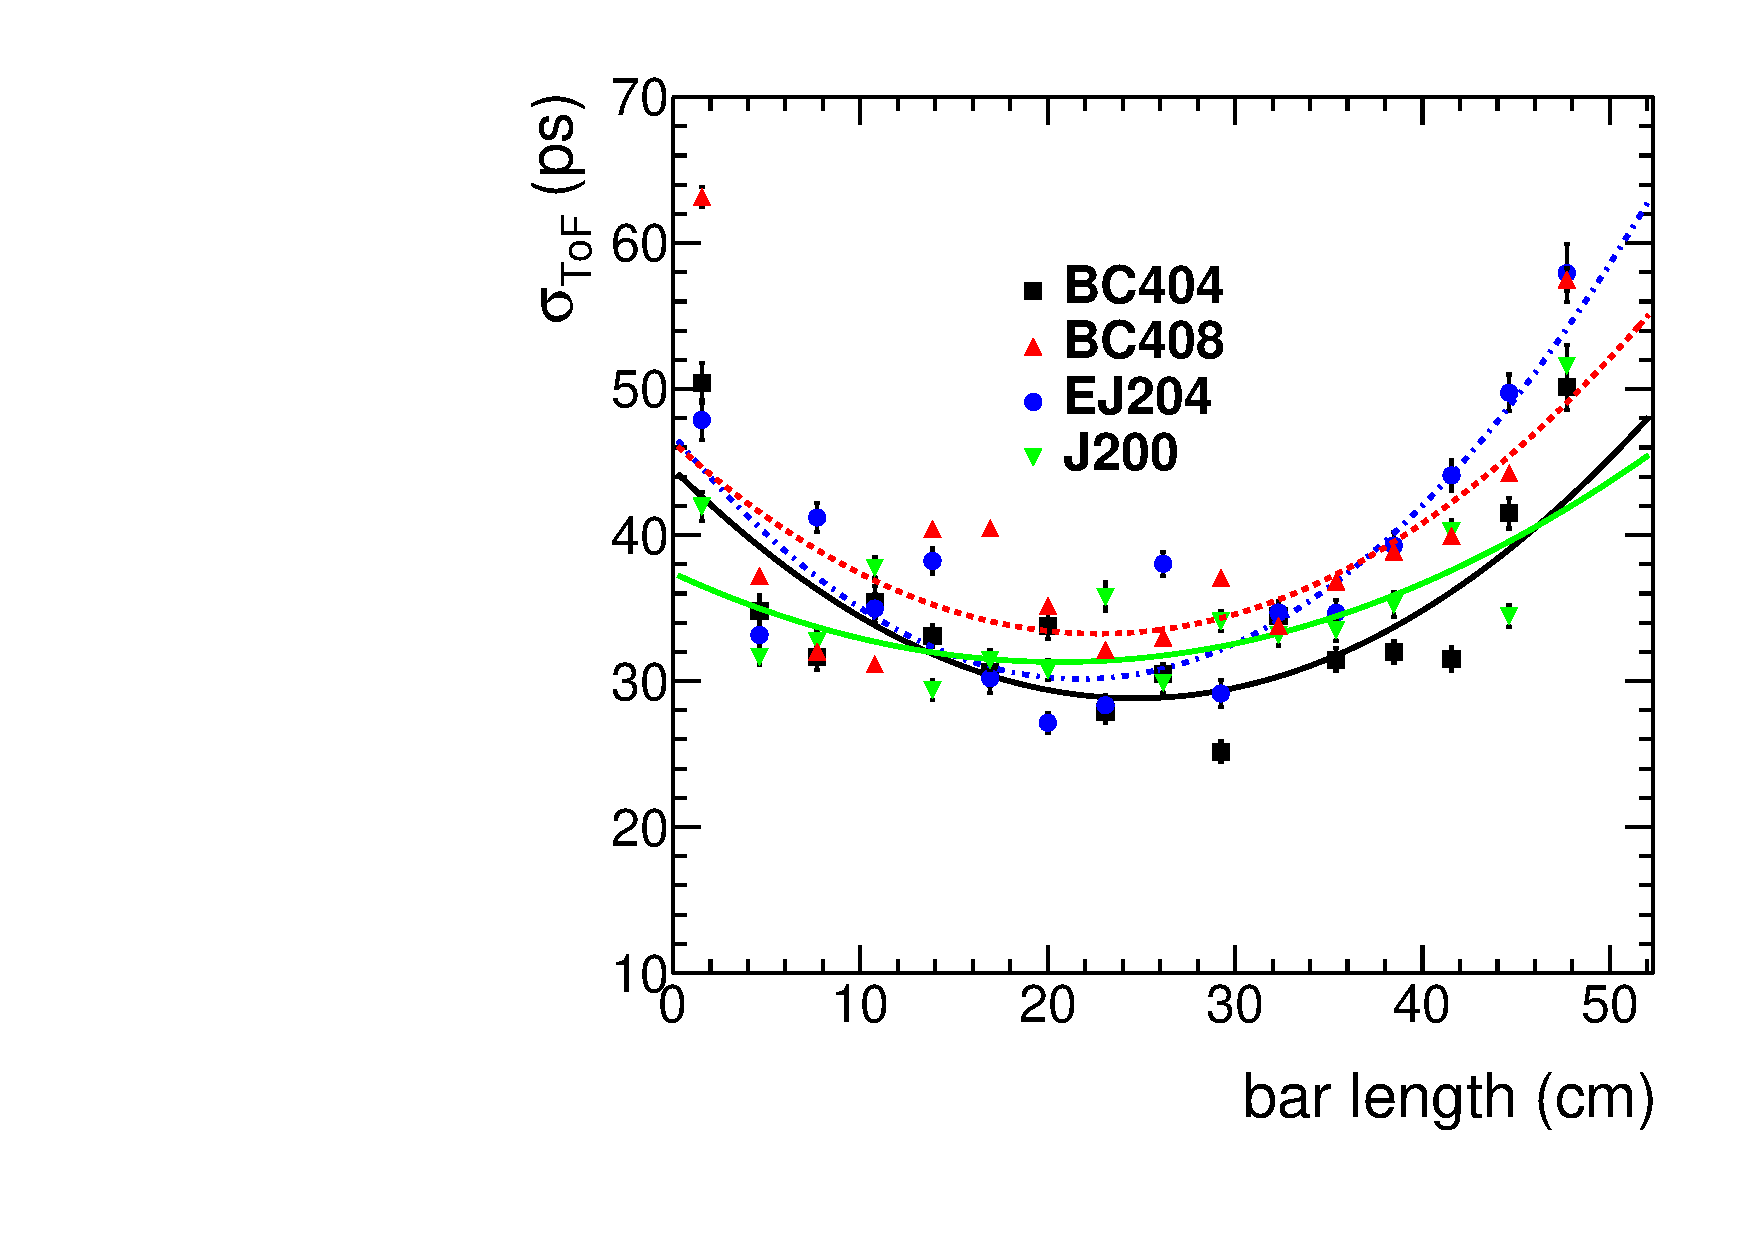
\includegraphics[width=13cm,height=10cm]{ye/fig_ye_scintillator/s0.pdf}}
\caption{The time resolution of different scintillator material (50cm scintillator bars )}
\label{f:TRmaterial}
\end{figure}

Initial measurements show that attenuation length values vary even among scintillation
bars of the same material and from the same mold, so in order to verify that
each counter meets required specifications, the attenuation length measurement is
incorporated into the unit testing of each counter constructed for Panel 1B. There are two methods used to measure the attenuation length. One is the cosmic ray method, which we use the same data collected in the three-bar time resolution measurements, described in Sec.III B. Figure~\ref{f:ADC} shows the Offset-corrected ADC values, which are directly proportional to the number of photons arriving at the photocathode are plotted against TDC difference values $(\frac{TDC_{L}-TDC_{R}}{2})(also called \Delta t)$ , which are proportional to the position through which the ionizing particles pass. To find the maximally occurring ADC value for each $\Delta t$ slice, ADC distributions for each TDC difference interval are fit with Gauss-convoluted Landau functions. The ADC provides a measure of the number of photons reaching the photocathode, and the left and right TDCs provide the time information needed to reconstruct the impact position based on the effective speed of light in the scintillator. The attenuation length parameters, TAL and BAL, of the scintillator are given by,
\begin{equation}
N=N_{0T}e^{-\frac{x}{\lambda_{T}}}+N_{0B}e^{-\frac{x}{\lambda_{B}}}
\label{eq:2}
\end{equation}
where $N_{0} = N_{0T} + N_{0B}$ is the initial number of photons caused by the cosmic ray passing
through the scintillator at the impact position $x$ and $N$ is the number of photons arriving
at the PMT. Figure~\ref{f:ADCTDC} illustrates the relationship between $N$ (ADC) and $x((TDC_{L}-TDC_{R})/2)$
for the data. Slices of the TDC difference values are projected onto the ADC axis, and fit
with Gauss-convoluted Landau functions from which the most probable ADC value for each
position is obtained (Fig.~\ref{f:ADC}). These new pairs of data points are fit by various ans\"{a}tze
of exponential functions to extract the attenuation length parameters, as shown in Fig.~\ref{f:expo}.
\begin{figure}[h!]
\begin{minipage}[h]{0.5\linewidth}
\centering
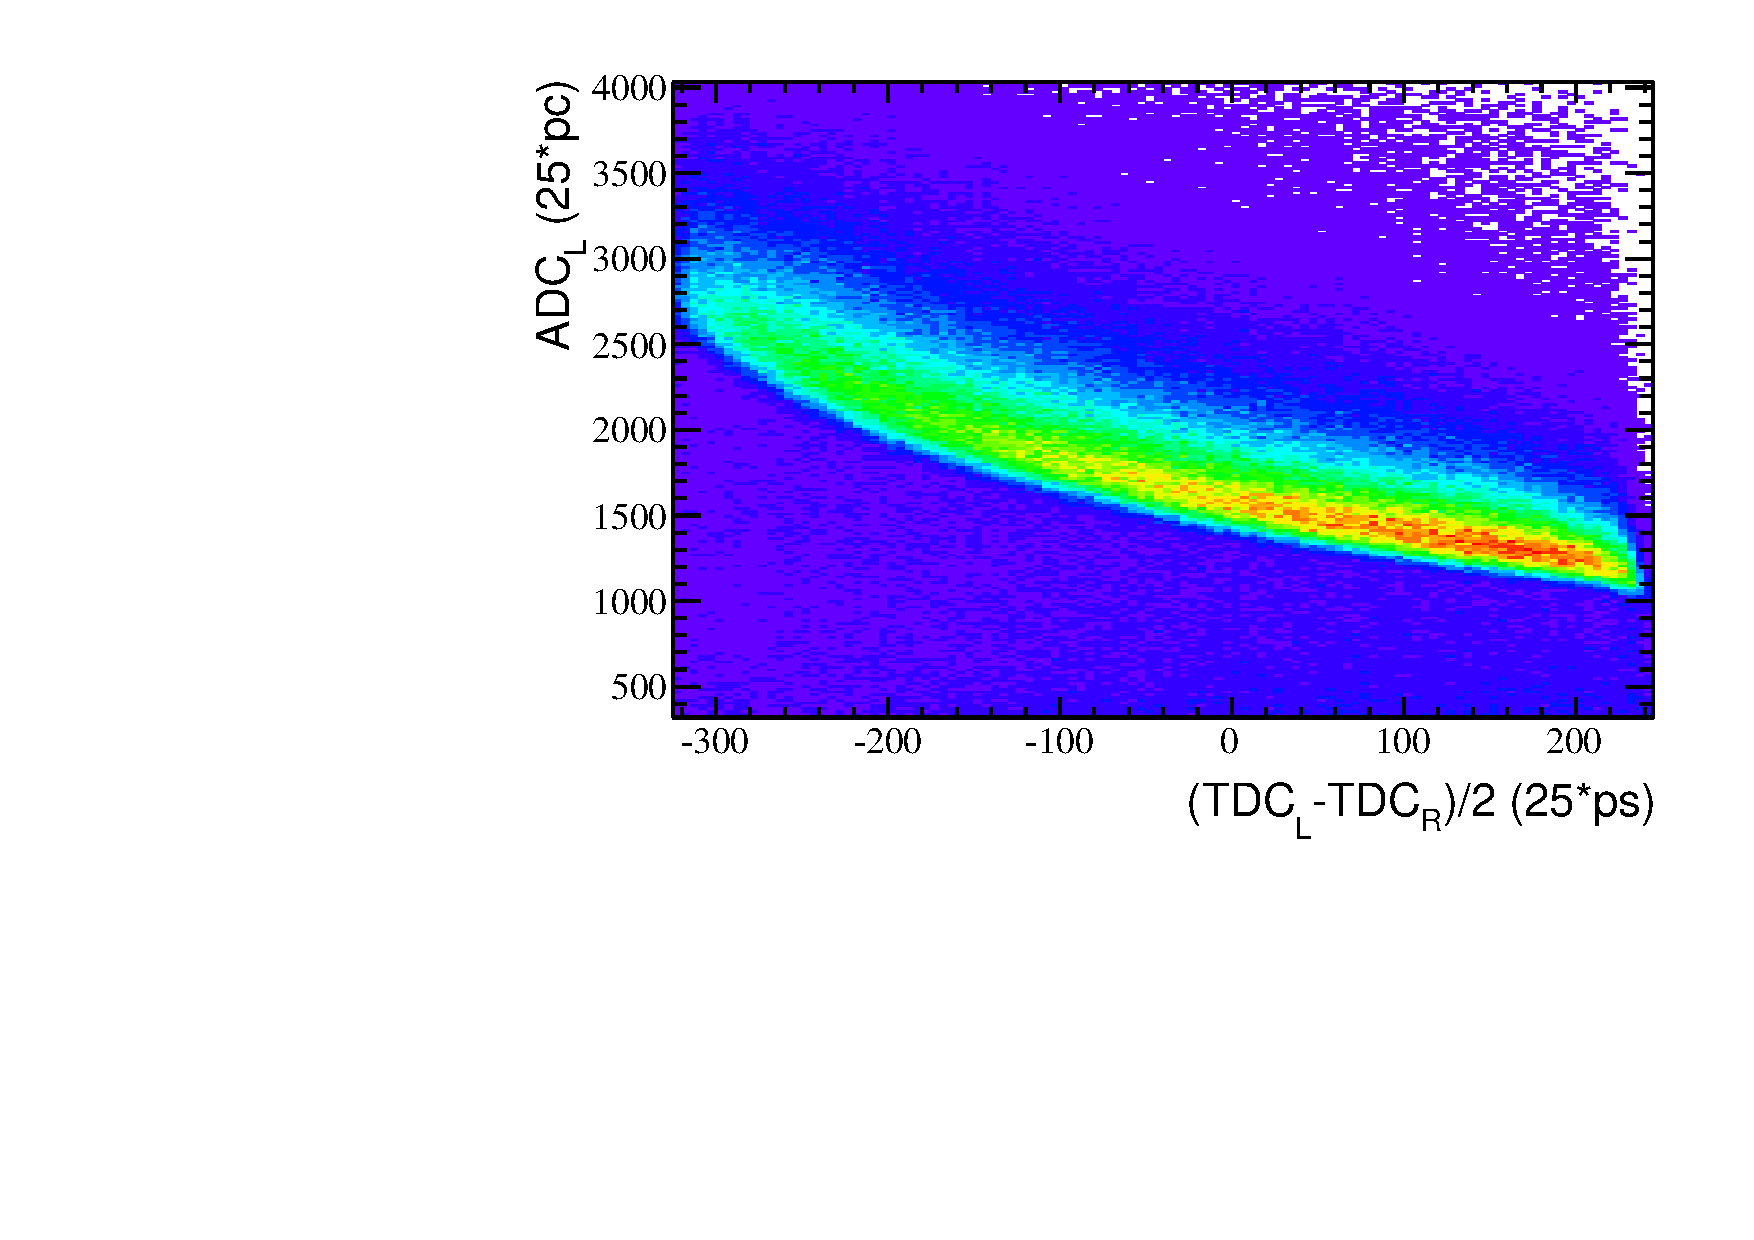
\includegraphics[width=2.5in]{ye/fig_ye_scintillator/c2_L.pdf}
\end{minipage}%
\begin{minipage}[h]{0.5\linewidth}
\centering
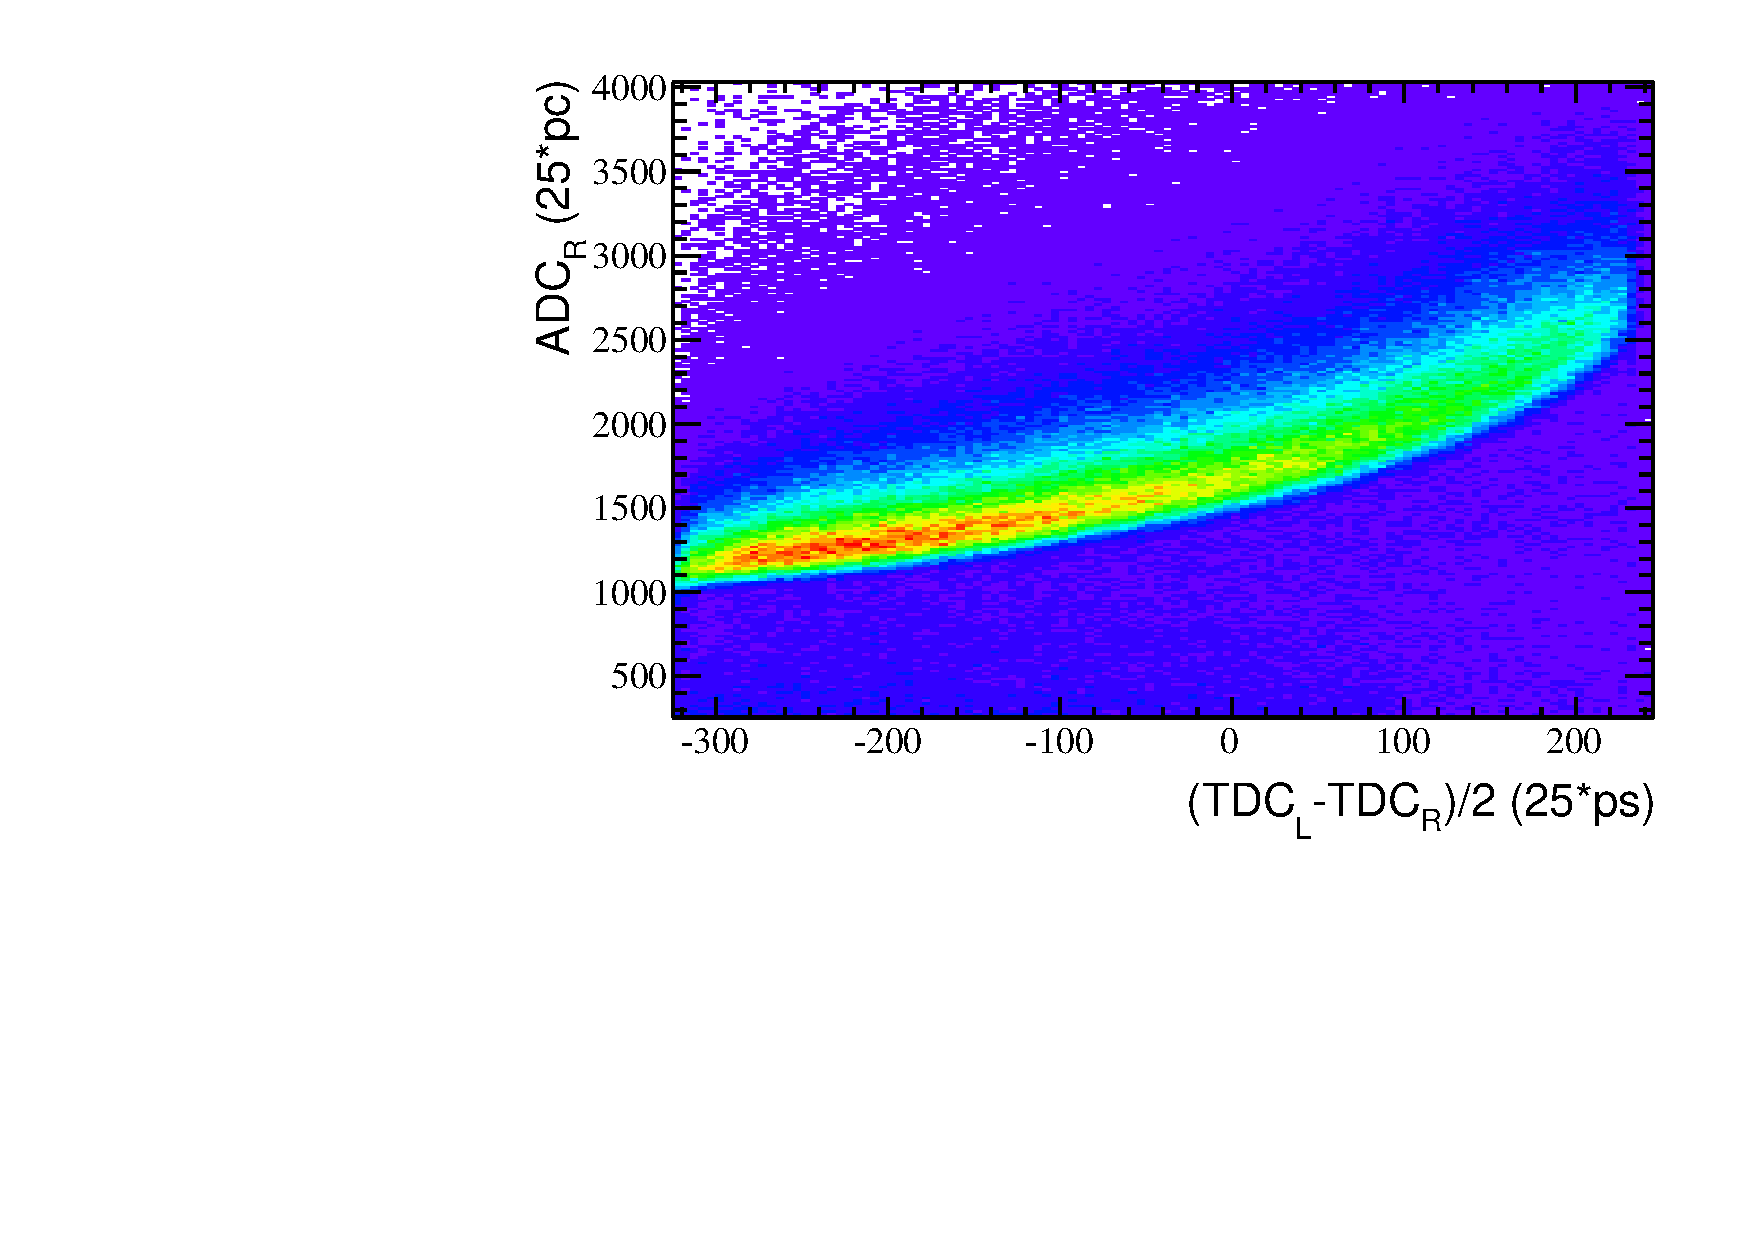
\includegraphics[width=2.5in]{ye/fig_ye_scintillator/c2_R.pdf}
\end{minipage}
\caption{Left and right $ADC_{L}$ and $ADC_{R}$ versus TDC difference for a $6cm\times6cm\times210cm$ bar}
\label{f:ADCTDC}
\end{figure}


And the other is the ource method, the $Sr-90$ source was put on the top of one scintillator at $5cm$ away from left side, then use the same electronic setups as three bar method. After the data satisfy the statistic requirement, move the source to the position of $15$cm away from left side of the bar and repeat the same step. For the position part, there is $10$cm away between each measurement position point. After the measurement, the data analysis steps are similar with the cosmic ray method, the only different is the ADC value which is subtracted by the cosmic ray signal background. After subtracting, fit the mean value of the ADC distribution of the fixed position versus the position distribution by the exponential function~\ref{eq:2} to get the TAL and BAL attenuation length, which shows in Fig.6. Here, it is a approvement that the attenuation length have two components, can not be fit well by the single exponential function.

\begin{figure}[ht!]
\centerline{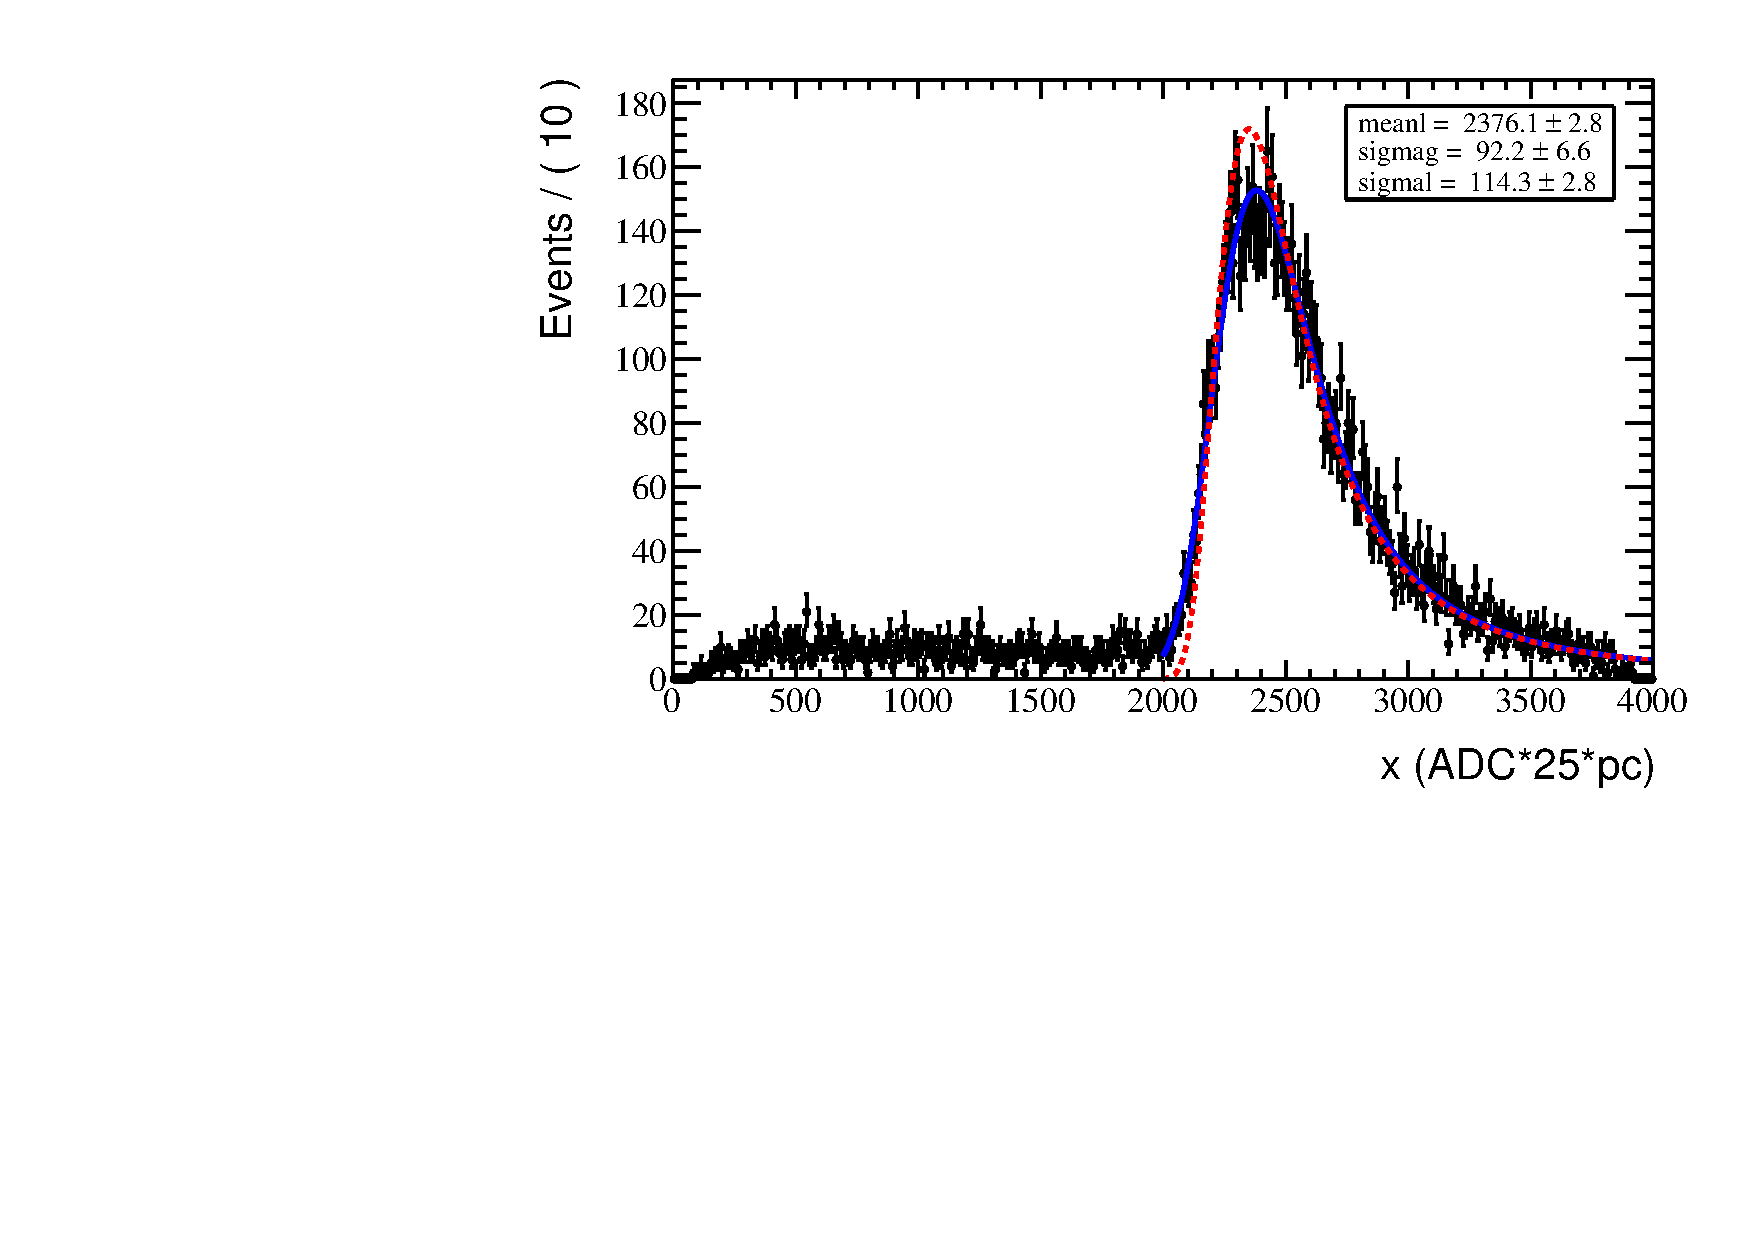
\includegraphics[width=13cm,height=10cm]{ye/fig_ye_scintillator/ADC.pdf}}
\caption{Gauss-convoluted Landau fit of the ADC distribution for a central single TDC difference
slice for the BC-408 210 cm-long bar, where x represents the ADC value, and "Maximum
x" is hence the most probable ADC value. The blue line shows Gauss-convoluted Landau fit, the red dashed line shows Landau fit only.
 }
\label{f:ADC}
\end{figure}


\begin{figure}[h!]
\begin{minipage}[h]{0.5\linewidth}
\centering
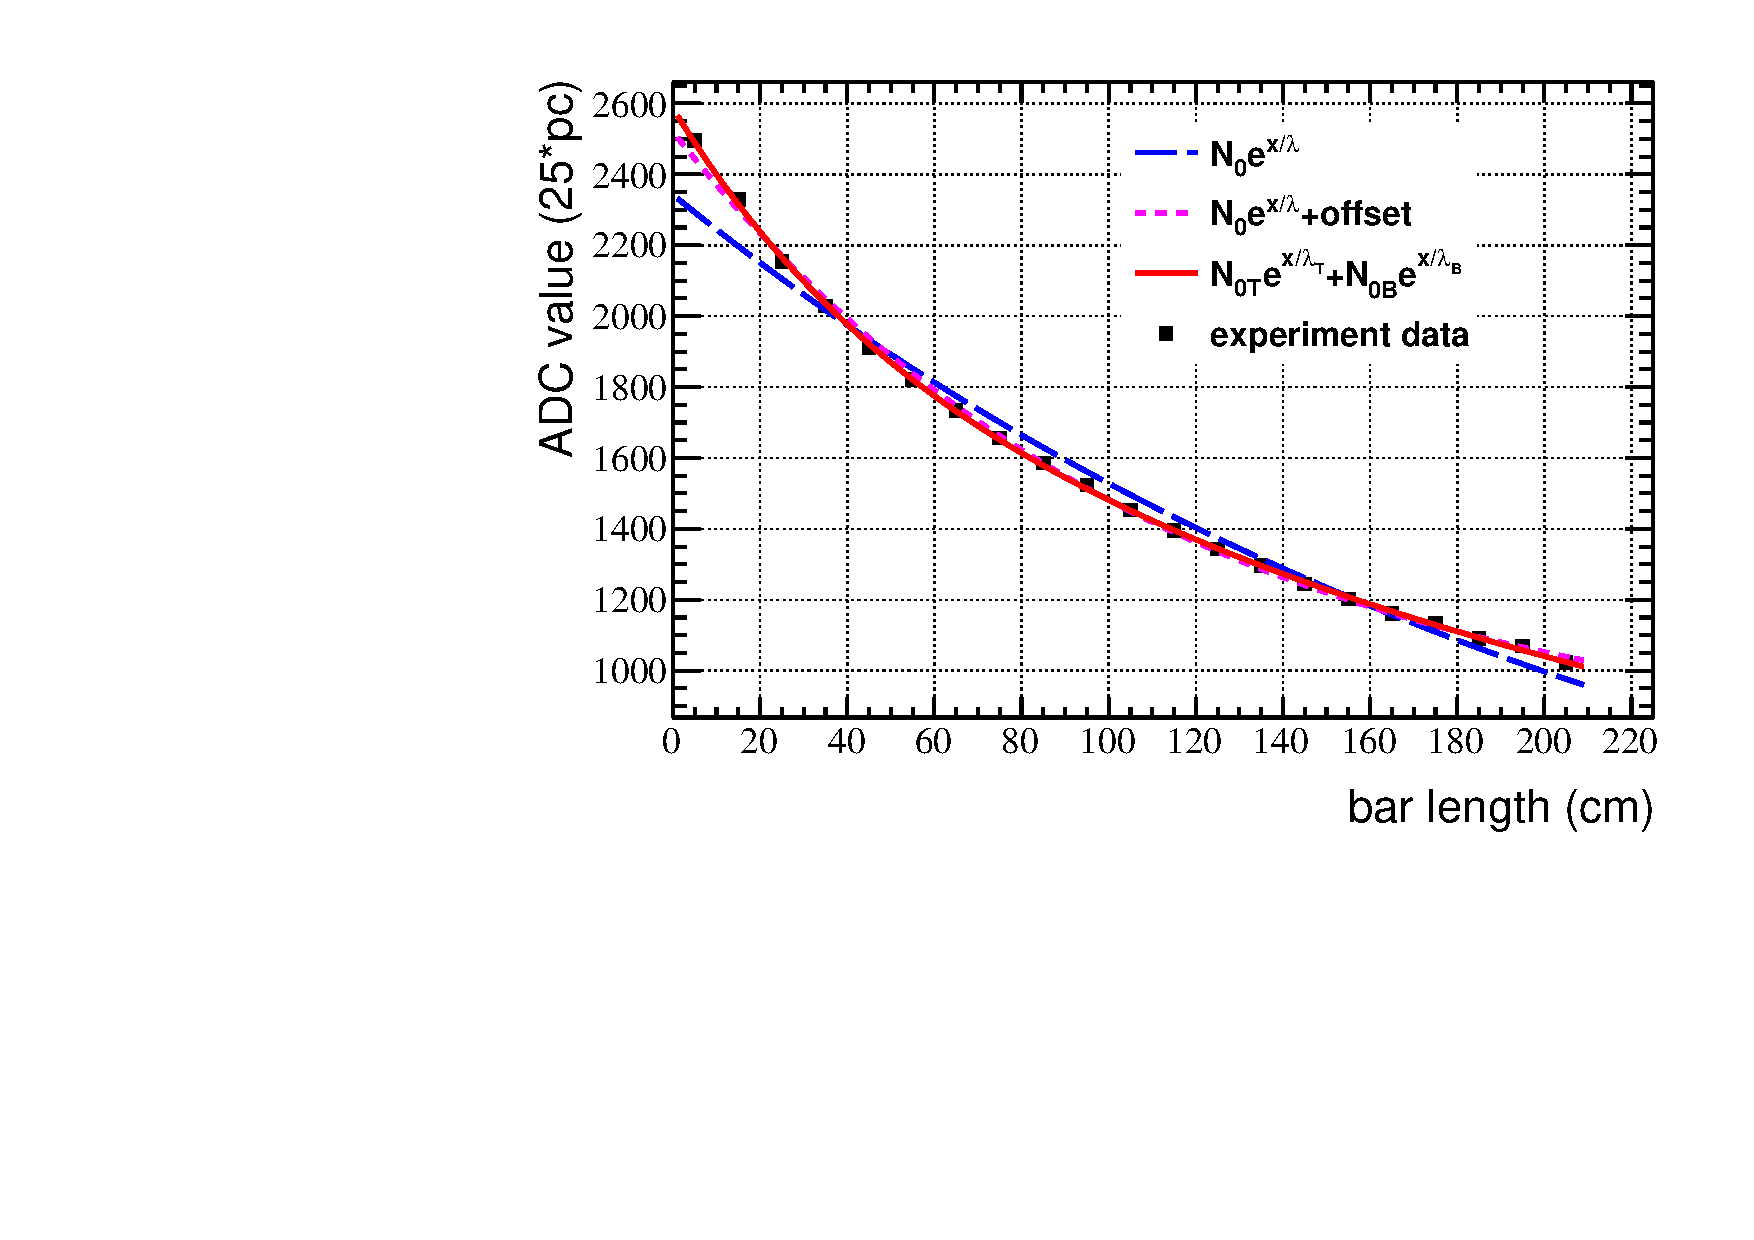
\includegraphics[width=3in]{ye/fig_ye_scintillator/c1_TL.pdf}
\end{minipage}%
\begin{minipage}[h]{0.5\linewidth}
\centering
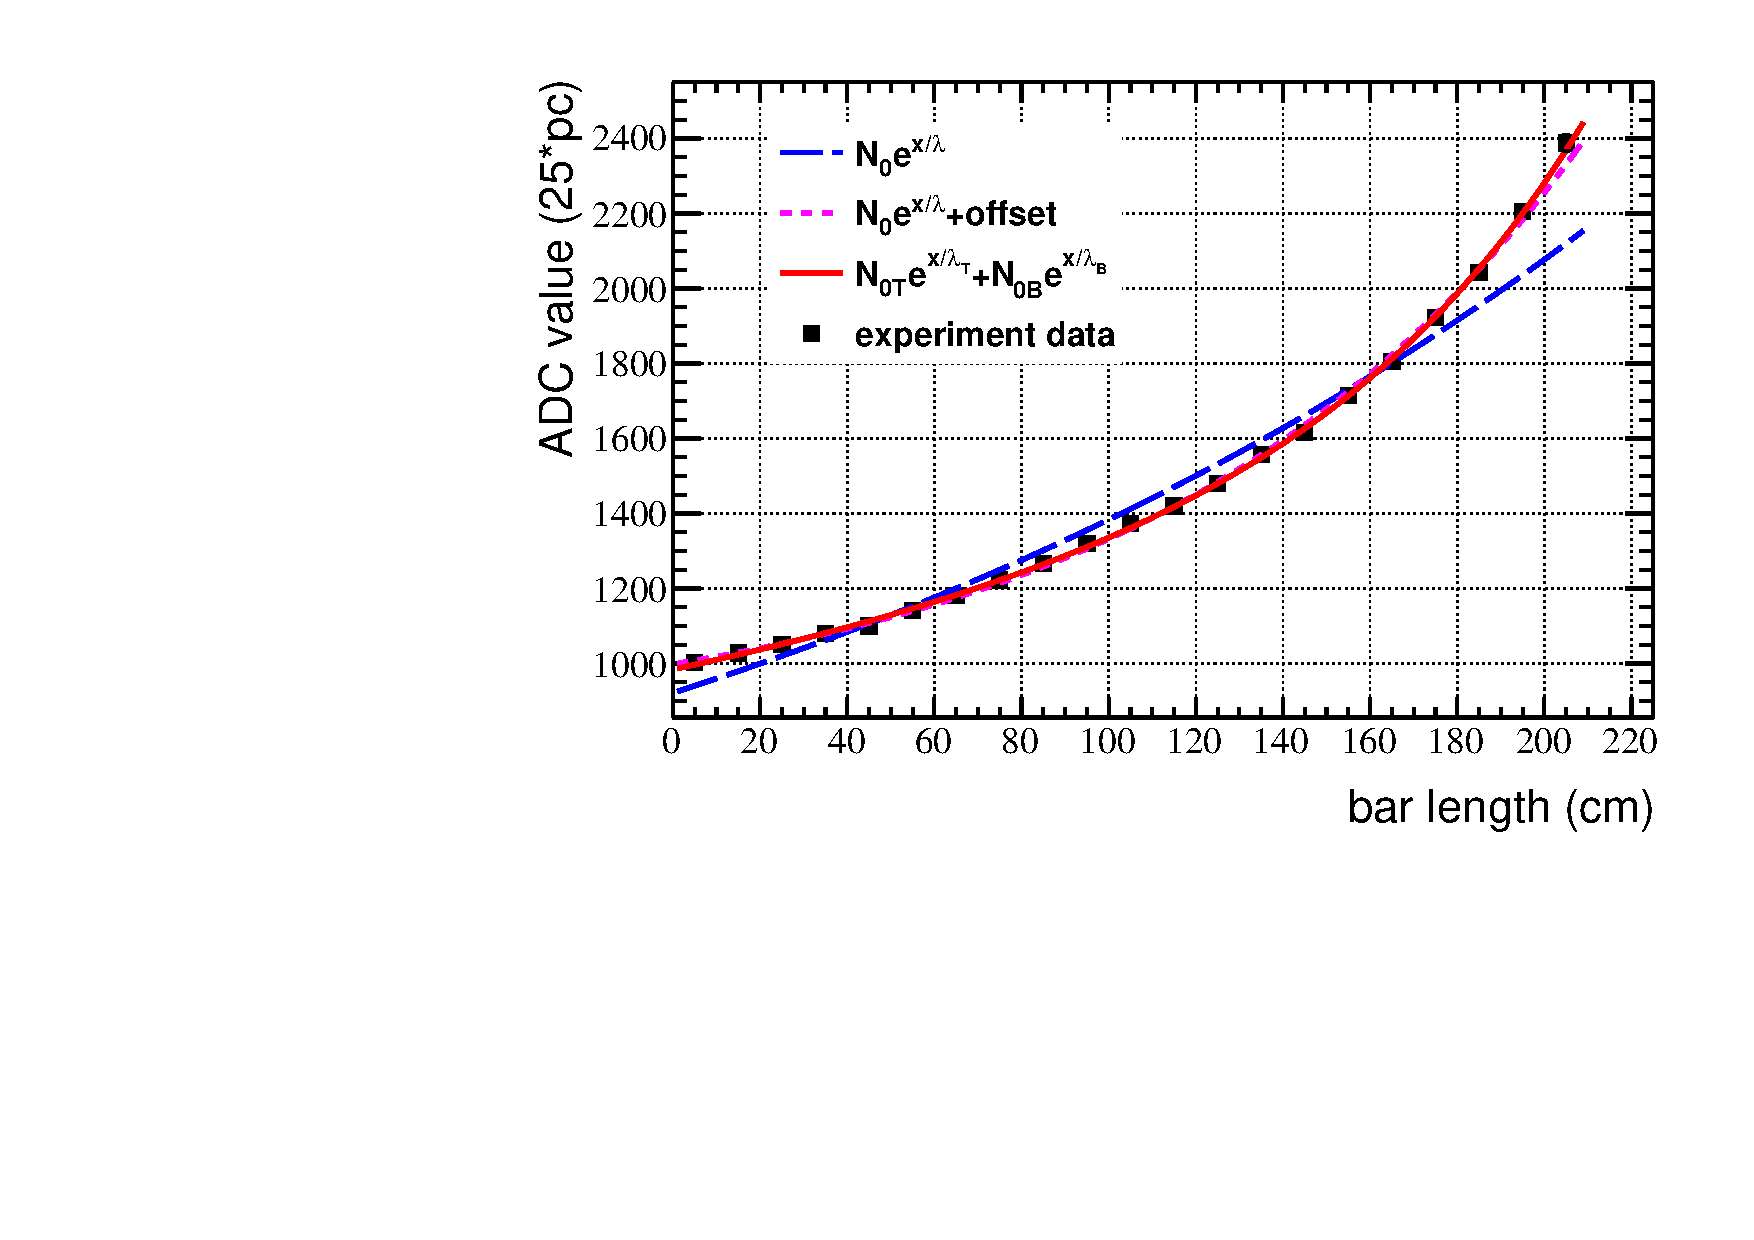
\includegraphics[width=3in]{ye/fig_ye_scintillator/c1_TR.pdf}
\end{minipage}

\caption{ADC versus TDC difference for the left and right PMTs of the $BC408$ $210 cm$-long bar. The black square shows most probable ADC value points corresponding to the bar length , the red line shows two exponential function fit, the blue long dashed line shows on exponential fit, the magenta short dashed line shows one exponential function with offset fit.}
\label{f:expo}
\end{figure}


Finally, in order to compare with the factory attenuation length value, we use two points method to get the attenuation length (same method as factory used to get their attenuation length value using laser system?). The two positions($15cm$ and $195cm$ away form the left side of the bar) are chosen to get the ADC values, and then fit this two data points by one exponential function to get the corresponding attenuation length. The comparison results are shown on Table~\ref{table2} and Table~\ref{table3}. we got consistent attenuation length value less than the factory value with both cosmic ray and source measurements, but for the first order acceptable. This is one of the quality check procedure.
\newpage
\begin{landscape}
\begin{table}[htbp]
\centering
\caption{Attenuation Length (AL) Table ($210$ cm bar) Source Method}
\begin{tabular}{|c|c|c|c|c|c|c|c|}
\hline
\multirow{2}{*}{Scintillator}
& \multirow{2}{*}{PMT}
& \multirow{2}{*}{2 points AL (cm)}
& \multirow{2}{*}{2 points AL (cm)}
& \multirow{2}{*}{2 points AL (cm)}
& \multirow{2}{*}{2 points AL (cm)}
& \multicolumn{2}{|c|}{21 points AL (cm)}\\
\cline{7-8}
type & Position & (15 and 195 cm) & (25 and 185 cm) & (35 and 175 cm) & (45 and 165 cm) & BAL & TAL \\
\hline
\multirow{2}{*}{LAL Factory AL}
& Left
& 178.09 $\pm$ 0.27
& 181.96 $\pm$ 0.34
& 185.98 $\pm$ 0.39
& 188.24 $\pm$ 0.46
& 250.03 $\pm$ 1.37
& 43.34 $\pm$ 0.47 \\
\cline{2-8}
(280cm) & Right & 238.06 $\pm$ 0.50 & 252.89 $\pm$ 0.63 & 261.51 $\pm$ 0.77
& 276.94 $\pm$ 1.00 & 332.33 $\pm$ 0.89 & 26.59 $\pm$ 0.20 \\
\hline
\end{tabular}
\label{table2}
\end{table}


\begin{table}[htbp]
\centering
\caption{Cosmic Ray Method}
\begin{tabular}{|c|c|c|c|c|c|c|c|}
\hline
\multirow{2}{*}{Scintillator}
& \multirow{2}{*}{PMT}
& \multirow{2}{*}{2 points AL (cm)}
& \multirow{2}{*}{2 points AL (cm)}
& \multirow{2}{*}{2 points AL (cm)}
& \multirow{2}{*}{2 points AL (cm)}
& \multicolumn{2}{|c|}{21 points AL (cm)}\\
\cline{7-8}
type & Position & (15 and 195 cm) & (25 and 185 cm) & (35 and 175 cm) & (45 and 165 cm) & BAL & TAL \\
\hline
\multirow{2}{*}{LAL Factory AL}
& Left
& 231.31 $\pm$ 8.09
& 234.95 $\pm$ 7.78
& 240.84 $\pm$ 9.51
& 241.45 $\pm$ 11.89
& 330.6 $\pm$ 43.1
& 48.3 $\pm$ 12.7 \\
\cline{2-8}
(280cm) & Right & 235.85 $\pm$ 8.61 & 240.33 $\pm$ 10.82 & 242.51 $\pm$ 11.00
& 241.97 $\pm$ 11.73 & 462.0 $\pm$ 167.1 & 58.8 $\pm$ 18.1 \\
\hline
\end{tabular}
\label{table3}
\end{table}

*AL---Attenuation Length                    *LAL---Long Attenuation Length
*2 points---1 exponential function method   *BAL---Bulk Attenuation Length
\end{landscape}
\newpage


\begin{figure}[ht!]
\centerline{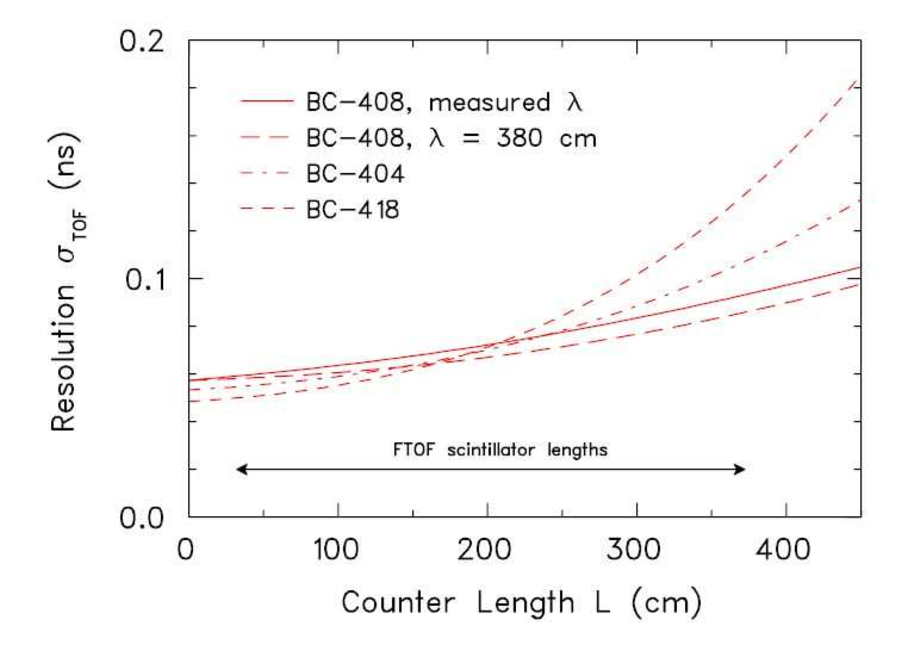
\includegraphics[width=13cm,height=10cm]{ye/fig_ye_scintillator/S2.pdf}}
\caption{Resolution for various scintillation materials showing the trad-off between attenuation length and decay time ~\cite{clasclas12}}
\label{f:tradeoff}
\end{figure}

\section{I Reflective wrap }


In order to maximize the internal reflection to get better time resolution, choosing the right wrapping material became important, so the following study was done for this purpose.
One BC404 $6 \times 6 \times 120${cm}$^3 $ scintillator is wrapped using one layer of aluminized Mylar and several layers of Tedlar. Another same size scintillator is wrapped using one layer of the white paper material and the same amount of Tedlar. Hamamatsu PMTs serial FA0413 and FA0389 are mounted to the left and right ends, respectively, of the scintillator with the VM2000 wrapping and aluminized Mylar wrapping material. The detector is then placed as the middle bar in the 3 bar setup and voltages are set so as to bring the point of inflection on the ADC histograms to around 1000. Thresholds are set to 75mV. Data is collected until 180000-200000 events are recorded.

By comparing the time resolution of a scintillator bar wrapped in the VM2000 material with it in aluminized Mylar material, Fig.~\ref{f:wrap} shows that the VM2000 material does not yield significantly better time resolutions than the aluminized Mylar material. It was also noted that the setup with the white paper wrapping required greater voltage to achieve points of inflection around 1000 on the ADC histograms. Finally, we decide to use the cheaper aluminized Mylar as the wrapping material.
\vspace{20mm}
\begin{figure}[h]
\centerline{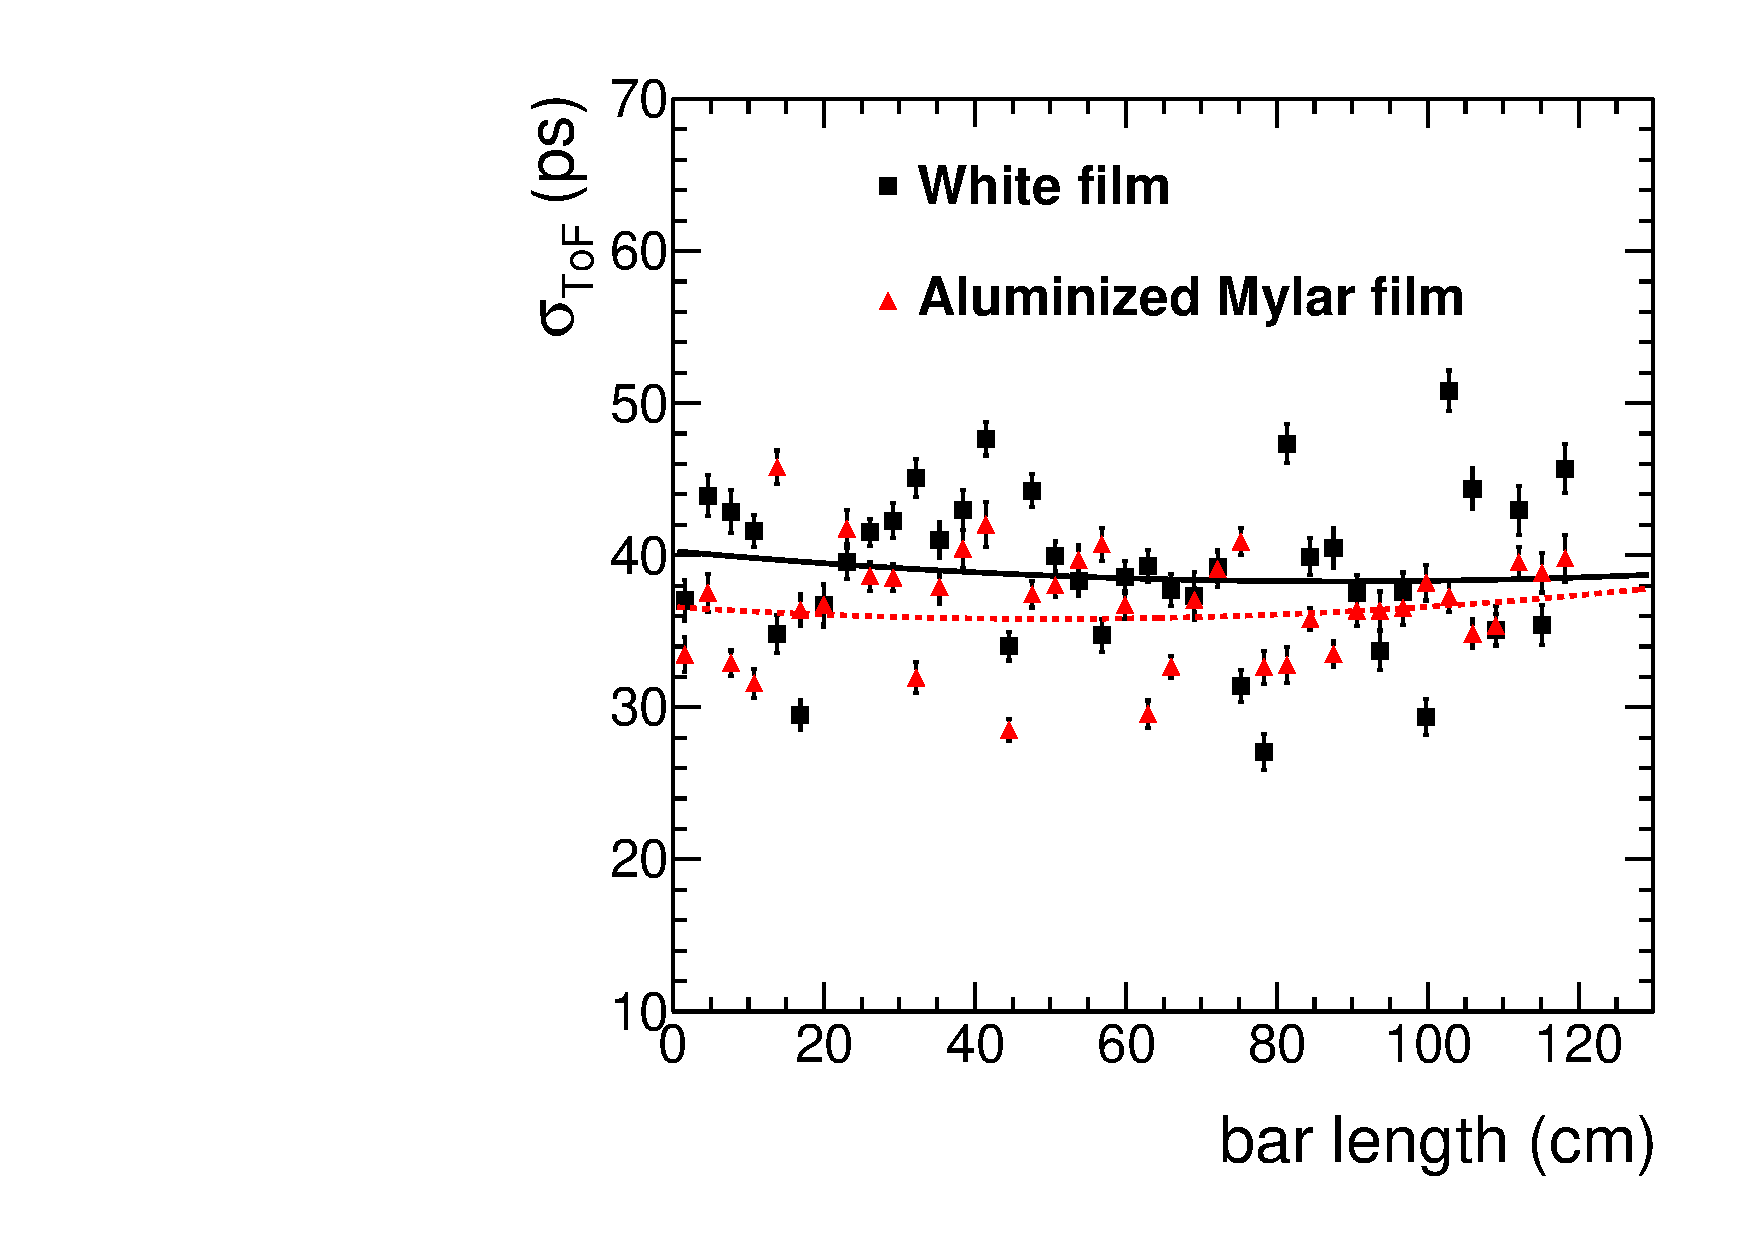
\includegraphics[width=13cm,height=10cm]{ye/fig_ye_wrap/R1.pdf}}
\caption{Wrap material}
\label{f:wrap}
\end{figure}


\section{
J Cables}

The primary concerns regarding choice of cable type are cost, space, and impact on time
resolution. Low-attenuation cables that maintain signal integrity over long distances cost
more and occupy more space. And the fast timing of signals from the FTOF system requires cables with low signal distortion also. With the cables of 768 PMTs~\cite{FToF12} being routed between the layers
and panels of the detector, the extra volume of bundled cables is a serious concern, so barring
an impact on time resolution, the thinner and less expensive RG58 cables are preferred.
The distortion and attenuation of signals through five different types of cable was investigated, including specification measurements of signal speed, attenuation, and rise time, which were all listed in the Table~\ref{T:table4}. After choosing the RG58 cable, the rise time and amplitude of the signal with RG58 cable length varied from $100\;ft$ to $500\;ft$ were measured, and the results are shown in Table~\ref{T:table6}.

Additionally, and most importantly, the time resolution tests were performed for various
lengths of cable RG58. The results are shown in Table~\ref{T:table5}, the time resolution does not change to bad even for $100$ feet-long cable. And with the digitization electronics at the panel edges, the
maximum cable lengths would be under 21 ft, for which RG58 is still well-suited.


\begin{table}[ht!]
\begin{center}
\begin{tabular}{|c|c|c|c|c|c|c|}
\hline
Cable Type &
Cable Length &
Delay Time &
Signal Speed &
Amplitude &
Rise Time &
Rise Time \\
 &
 &
 &
 &
 &
($30\%$ to $70\%$) &
($10\%$ to $90\%$)

 \\
\hline
RG-9913& 	251.5 ft.   &	303.7 ns 	&            25.24 cm/ns 	&      1.4 V &      1.78 ns & 10.55 ns	 \\
RG-8& 	    202.2 ft. 	&   310.6 ns 	&            19.84 cm/ns 	&      1.432 V &    2.69 ns & 12.69 ns\\
RG-174& 	128.2 ft. 	&   198.35 ns 	&            19.7 cm/ns 	&      1.072 V &    4.30 ns & 18.03 ns	 \\
RG-214& 	95.3 ft. 	&   147.4 ns 	&            19.71 cm/ns 	&      1.464 V &    1.36 ns & 7.01 ns\\
RG-58& 	    200 ft. 	&   323.3 ns 	&            18.86 cm/ns 	&      1.41 V &     5.67 ns &22.04 ns\\
\hline
\end{tabular}
\end{center}
\caption{Individual cable comparison table (gate width:$ 80 ns$)}
\label{T:table4}
\end{table}


\begin{table}[ht!]
\begin{center}
\begin{tabular}{|c|c|c|c|}
\hline
Cable Length &
Amplitude &
Rise Time &
Rise Time \\
 &
 &
($30\%$ to $70\%$) &
($10\%$ to $90\%$)


 \\
\hline
5  ns     &	1.55 V  &          0.36 ns & 1.05 ns   \\
50 ft.     &	1.54  V 	&     1.03 ns & 5.37 ns   \\
75 ft.     &	1.50  V 	&      1.9 ns & 10.94 ns   \\
100 ft.     &	1.47  V 	&          2.80 ns & 15.39 ns   \\
200 ft. 	&   1.42 V 	&          7.20 ns & 37.77 ns     \\
300 ft. 	&   1.36 V 	&          12.88 ns & 56.87 ns	\\
400 ft. 	&   1.28 V 	&          18.34 ns & 76.22 ns   \\
500 ft. 	&   1.24  V 	&          24.65 ns &93.38 ns   \\
\hline
\end{tabular}
\end{center}
\caption{Variable length comparison results of RG58 cable (gate width:$ 80 ns$)}
\label{T:table6}
\end{table}

\begin{table}[htbp]
\begin{center}
\begin{tabular}{|c|c|}
\hline
Cable Length &
\multicolumn{1}{|c|}{Time Resolution}\\
\hline
50 ft.  & 36.16ps\\
75 ft.  & 36.53ps\\
100 ft. & 34.37ps\\
\hline
\end{tabular}
\end{center}
\caption{ Time resolution results of 100cm reference bars with different $RG-58 $ cable length }
\label{T:table5}
\end{table}




\section{
F Counter construction and testing process}

 The CLAS12 panel 1b detector has $62$ counters. Each counter contain one scintillation bar wrapped with aluminized Mylar film and two PMTs covered with magnetic shielding boxes. For counter assembly, each end of the scintillator is fitted with black tape (hereon referred to as "anticookie"), which masks the corners while leaving a circular window that extends one millimeter into the area that will be covered by the PMT. Apply approximately 1 $ml$ of glue to the top end of a scintillator, straight down in the center of the anticookie. Check for bubbles in glue. Since the bubbles between scintillation bars and PMTs can influence the time resolution, reapply glue to avoid bubbles. Lower the PMT in a rotating motion through the centering tools slowly onto the scintillators.

After gluing two PMTs on the end of one scintillator, the Tedlar film was wrapped the counter tightly and wrinkle-free in three layers. Retain the film
tension with electrical tape, secured only on the front side. Finish it off with a
layer of the 5-cm wide, thin, black tape running the full length of the Tedlar
sheet to avoid peeling off . Wrap 2 layers of electrical tape around PMT about $3$ cm from edge of scintillator
and at end near wires. Firmly pigtail the Tedlar film as close as reasonably possible to the PMT high voltage (HV) divider in the center with the electrical tape, trim the Tedlar to 3 cm from the
PMT HV divider, and finish the pigtail by wrapping the electrical tape around
the bundled Tedlar and cables extending to 5 cm beyond the PMT HV divider. Check that the ends closest to the PMT of the Tedlar pigtail are less than $15.5$mm in diameter in order to pass through the cable hole of the magnetic shielding box. Zip tie wires tightly using pliers at base of PMT and trim excess.

Repeat above steps for the same length six bars, then ensure that the six counters are properly aligned and secured in the six-bar rack. Connect HV, anode, and dynode cables, each set from top-left, labeled 1 to bottom-right, labeled 12. Apply baseline voltages according to PMT testing task database entries. Verify that the anode and dynode signals on the oscilloscope match the nominal documented pulse-shape distribution. Verify that the dark current is independent of light on/off status. And then start to take test run. After enough statistic data taken, the automated analysis program (section IV part G) will get the attenuation length and the time resolution of the individual counter and saved them in the database.

The backing structure is designed to support the counters in the detector space, each backing structure holds two neighbor length counters , which shows in Fig.~\ref{f:tape-rep}. There is a single-sided rubber tape between the backing structure and counters, which is in order to prevent counters to move around. Lefthanded and righthanded double-sided fiberglass tape loops, running side-by-side extending from the back corner along the back, the side, and then across the top surfaces in opposite directions, which shows in Fig.~\ref{f:tape4}, binds two counters and the backing structure tightly together. Figure~\ref{f:sector31} shows the example of double-sided fiberglass tape distribute in one backing structure precisely. Since two scintillators have different length, the close end position can only tolerate one single direction tape loop.  Then applying a single-sided, red Mylar tape loop, with both ends terminating on the back of the backing structure, to cover the double-sided fiberglass tape to avoid the peeling, which shows in Fig.~\ref{f:tape2}. After considering the room tolerance between scintillators, it is important to make sure there is no overlapping tape loop between all backing structure. The nice whole tape loop distribution for all counters is shown in Fig.~\ref{f:allsector}. Repeat above taping steps for all backing structure and assemble them as six sectors, one of them shows in Fig.~\ref{f:allsector}.

\begin{figure}[h!]
\centerline{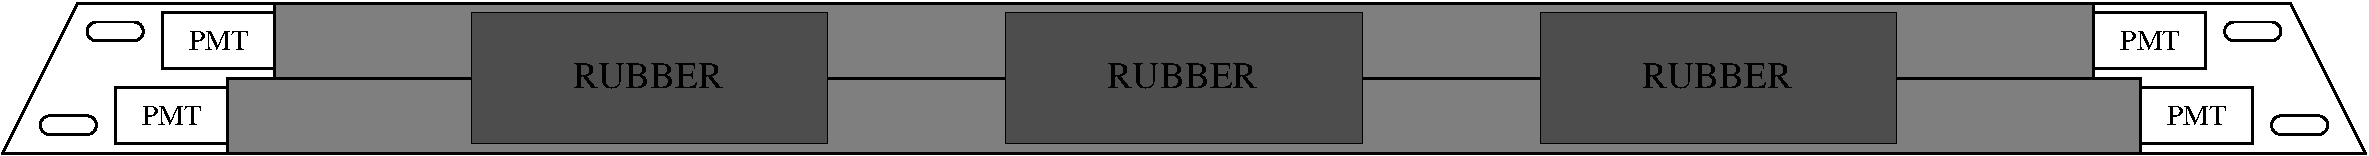
\includegraphics[width=15cm,height=1cm]{ye/fig_ye_construction/tape-replace.pdf}}
\caption{Counter structure}
\label{f:tape-rep}
\end{figure}

\begin{figure}[h!]
\begin{minipage}[h]{0.5\linewidth}
\centering
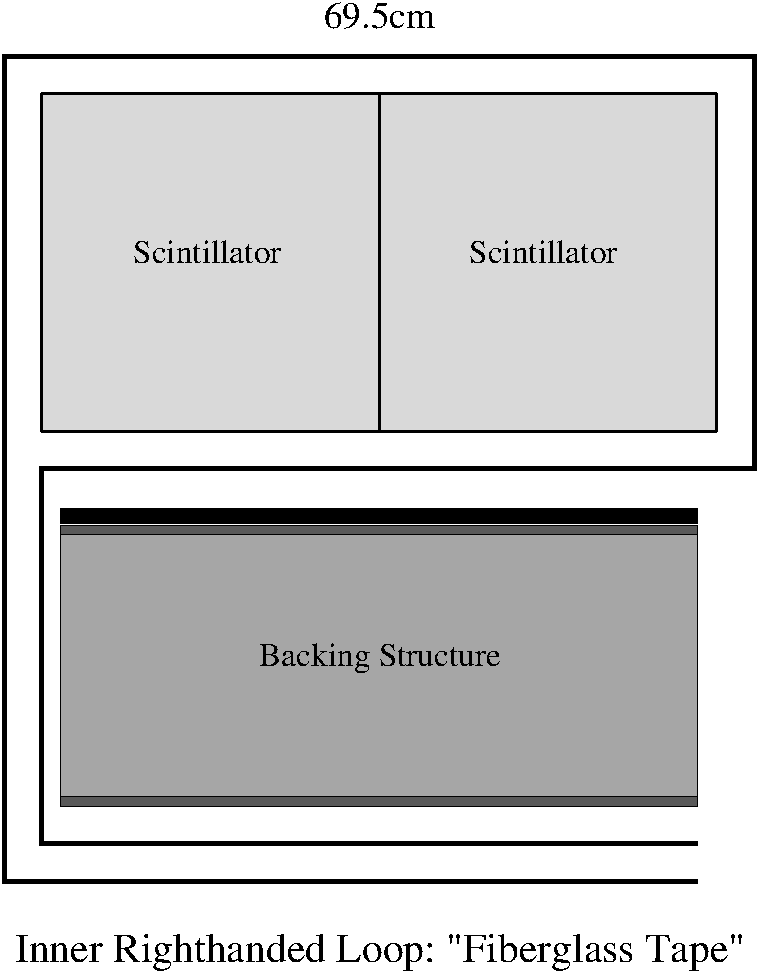
\includegraphics[width=2.0in]{ye/fig_ye_construction/fig-tape4.pdf}
\end{minipage}%
\begin{minipage}[h]{0.5\linewidth}
\centering
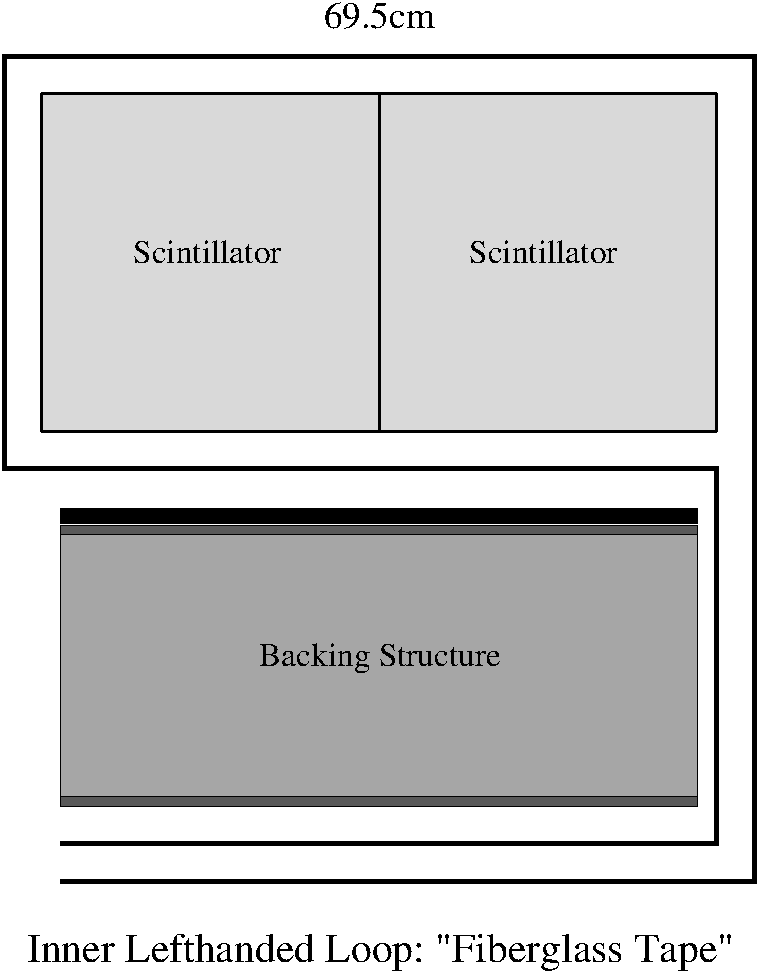
\includegraphics[width=2.0in]{ye/fig_ye_construction/fig-tape3.pdf}
\end{minipage}
\caption{Taping direction}
\label{f:tape4}
\end{figure}

\begin{figure}[h!]
\centerline{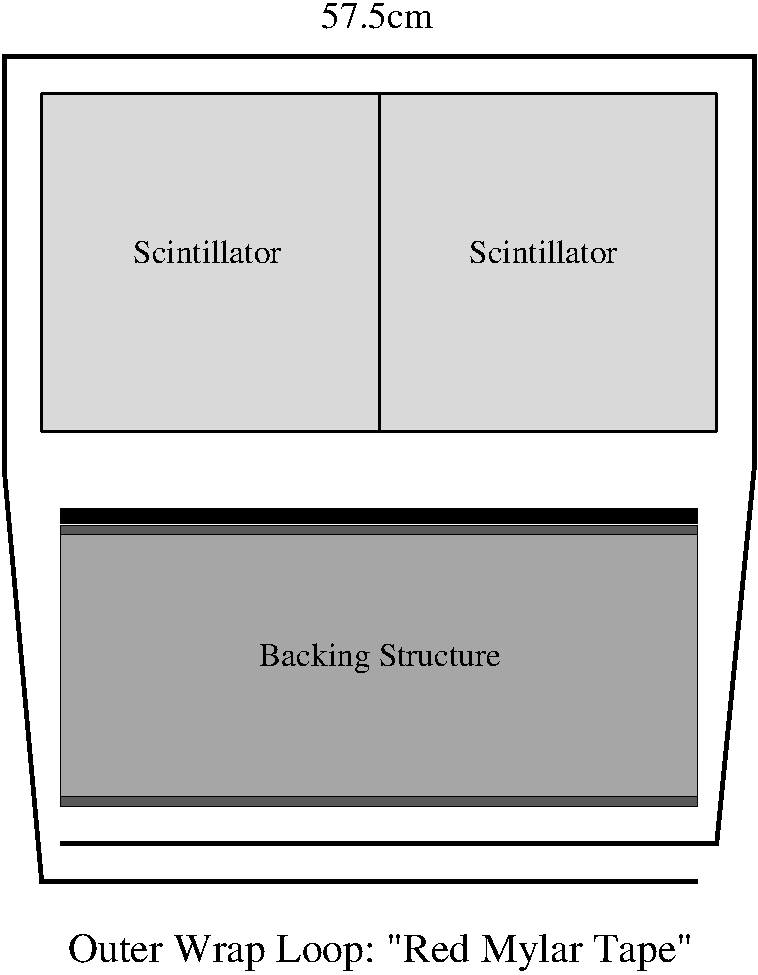
\includegraphics[width=5cm,height=7cm]{ye/fig_ye_construction/fig-tape2.pdf}}
\caption{Counter structure}
\label{f:tape2}
\end{figure}


\begin{figure}[h!]
\centerline{\includegraphics[width=18cm,height=4cm]{ye/fig_ye_construction/sector-31-wraping.pdf}}
\caption{wrapping example of sector 31 }
\label{f:sector31}
\end{figure}
\newpage
\begin{figure}[h!]
\centerline{\includegraphics[width=18cm,height=18cm]{ye/fig_ye_construction/sector.pdf}}
\caption{Final taping structure of all sectors }
\label{f:allsector}
\end{figure}
\newpage


The following section is relate to the technical detail about PMT testing, counter assembly and testing. It can be escaped.

%%\section{
PMT testing, counter assembly and testing technical detail}

PMT Testing\\

$\bullet$ AT NO TIME SHOULD THE BOX BE OPEN WHILE THE HV IS ON!\\
$\bullet$ AT NO TIME SHOULD HV EXCEED 1750!\\
$\bullet$ Unpack PMT and load PMT into and close black box, insert Sr-90 source into
designated cavity as needed, and connect HV (do NOT turn it on yet) and signal
cables.\\
$\bullet$ Apply optical grease to PMT as needed.\\
$\bullet$ Pull back and secure the \\
$\bullet$ Insert the PMT into the box with the ground oriented up and carefully press the
PMT forward against the scintillator until flush, as indicated by the oozing of the
grease from around the PMT\\
$\bullet$ Secure PMT in black box using rubber bands and release the sled allowing it to
slide forward.\\
$\bullet$ 1500V dark current\\
$\bullet$ Set the HV to 1500V, be as accurate as possible when setting the voltage for
this and all other steps. After configuring the electronics, take Dark Current
measurements for 1500V.\\
$\bullet$ Remove the source.\\
$\bullet$ Feed the anode signal into the Linear FiFo; one output going to the
discriminator with a threshold of 10mV and output directly to a visual scalar.
The second output should go to the oscilloscope.\\
$\bullet$ For scalar measurements, remove the VETO for 100 seconds and record the
count on the scalar\\
$\bullet$ For Oscilloscope measurements, set vertical scale to 20mV, adjust trigger to
10mV, and take a range of frequency values and average\\
$\bullet$ 1500V ADC\\
$\bullet$ Record (ADC mean - offset mean).\\
$\bullet$ Perform 2 times.\\
$\bullet$ For ADC measurements use the voltage splitter at 1500V even if not needed\\
$\bullet$ Baseline ADC\\
$\bullet$ adjust HV to baseline\\
$\bullet$ Record (ADC mean - offset mean).\\
$\bullet$ Perform 2 times.\\
$\bullet$ For ADC measurements use the voltage splitter even if not needed\\
$\bullet$ Baseline rate of events\\
$\bullet$ Feed the anode signal with source into Linear FiFo; one output going to the
discriminator with a threshold of 10mV and output directly to a visual scalar.
The second output should go to the oscilloscope.\\
$\bullet$ For scalar measurements, remove the VETO for 100 seconds and record
the count on the scalar\\
$\bullet$ For Oscilloscope measurements, set vertical scale to 20mV, adjust trigger
to 10mV, and take a range of frequency values and average\\
$\bullet$ Baseline dark current\\
\begin{figure}[ht!]
\centerline{\includegraphics[width=8cm,height=6cm]{ye/fig_ye_pmt_test/dark_curr_measured.pdf}}
\caption{Measured dark current }
\label{f:dark_measure}
\end{figure}

\begin{figure}[ht!]
\centerline{\includegraphics[width=8cm,height=6cm]{ye/fig_ye_pmt_test/dark_curr_factory.pdf}}
\caption{Factory dark current }
\label{f:dark_factory}
\end{figure}

\begin{figure}[ht!]
\centerline{\includegraphics[width=8cm,height=6cm]{ye/fig_ye_pmt_test/dark_curr_ratio.pdf}}
\caption{Factory and measured dark current ratio }
\label{f:dark_ratio}
\end{figure}
$\bullet$ Feed the anode signal into the Linear FiFo; one output going to the
discriminator with a threshold of 10mV and output directly to a visual scalar.
The second output should go to the oscilloscope.\\
$\bullet$ For scalar measurements, remove the VETO for 100 seconds and record
the count on the scalar\\
$\bullet$ For Oscilloscope measurements, set vertical scale to 20mV, adjust trigger
to 10mV, and take a range of frequency values and average\\
$\bullet$ Baseline snapshot\\
$\bullet$ 1500 snapshot\\
$\bullet$ 1700 snapshot\\
$\bullet$ 1500 rate of events\\
$\bullet$ Feed the anode signal with source into the Linear FiFo; one output going to
the discriminator with a threshold of 10mV and output directly to a visual
scalar. The second output should go to the oscilloscope.\\
$\bullet$ For scalar measurements, remove the VETO for 100 seconds and record
the count on the scalar\\
$\bullet$ For Oscilloscope measurements, set vertical scale to 20mV, adjust trigger
to 10mV, and take a range of frequency values and average\\
$\bullet$ 1500 dark current\\
$\bullet$ Feed the anode signal into the Linear FiFo; one output going to the
discriminator with a threshold of 10mV and output directly to a visual scalar.
The second output should go to the oscilloscope.\\
$\bullet$ For scalar measurements, remove the VETO for 100 seconds and record
the count on the scalar\\
$\bullet$ For Oscilloscope measurements, set vertical scale to 20mV, adjust trigger
to 10mV, and take a range of frequency values and average\\
$\bullet$ Rise time\\
$\bullet$ Plug into oscilloscope and read off the numbers\\
$\bullet$ Note: All measurements using the splitter or attenuators will result in values
that are one half (for the splitter) or a fraction of (variable based on the
attenuator) their actual value\\
$\bullet$ Add test results and notes to corresponding database entry. All measurements
should have corresponding Oscilloscope snapshots and histograms where
applicable.\\
$\bullet$ Remove any grease from black box at end of day.\\
\begin{figure}[ht!]
\centerline{\includegraphics[width=8cm,height=6cm]{ye/fig_ye_pmt_test/gain.pdf}}
\caption{gain}
\label{f:gain}
\end{figure}


\begin{figure}[ht!]
\centerline{\includegraphics[width=8cm,height=6cm]{ye/fig_ye_pmt_test/alpha.pdf}}
\caption{alpha}
\label{f:alpha}
\end{figure}

Counter Assembly\\
$\bullet$ Crew size: 2-3, depending on length.\\
$\bullet$ Prepare and clean workbench area, and retrieve six identical-length scintillators
from storage area.\\
$\bullet$ Use latex gloves before further handling the scintillators.\\
$\bullet$ Remove protective film only at the end faces of the scintillators.\\
$\bullet$ Each end of the scintillator is fitted with black tape (hereon referred to as
"anticookie"), which masks the corners while leaving a circular window that
extends one millimeter into the area that will be covered by the PMT. Apply
anticookie end window.\\
$\bullet$ Mask the scintillator around top edges of protective tape with electrical tape
slightly above the top edge. Fold the tape down to prevent glue driping.\\
$\bullet$ Place the scintillators Diamond cut side facing you horizontally into the
windmill frame while maintaining a balanced load.\\
$\bullet$ Pressurize the air pistons to $40$ psi to secure the scintillators in place.\\
$\bullet$ Use the hydraulic lift to raise the windmill frame, clearing it for rotation, and
rotate so that the scintillators are vertically aligned.\\
$\bullet$ Secure height and rotation angle, and keep the compressor powered.\\
$\bullet$ Mount centering tool with open side facing you. Leave a $1.5\;cm$gap between
the top of the scintillator and the centering tool for easy centering.\\
$\bullet$ Extract $7.4 \;ml$ of each of scintillator glue and $2.4\; ml$ of catalyst using disposable
syringes and squirt the content into a disposable mixing container.\\
$\bullet$ Mix and pour glue into a capped syringe with its stopper removed and mount it
into one of the base holes in the vacuum chamber and seal.\\
$\bullet$ Close all valves and open valve to chamber from pump. Evacuate chamber to
 $30$ psi. Close valve, turn pump off, and wait for 2 minutes. Open release valve
on pump farthest from chamber to protect pump from condensation. Open
release valve on chamber to restore pressure, and wait 2 minutes. Close all
valves.\\
$\bullet$ Wrap paper towel around bottom base of centering to catch excess glue.\\
$\bullet$ Prepare PMT for glueing.\\
$\bullet$ Place stopper in syringe and squeeze out any remaining air from tip.\\
$\bullet$ Apply approximately 1 ml of glue to the top end of a scintillator, straight down
in the center of the anticookie.\\
$\bullet$ Check for bubbles in glue. If bubbles are found reapply glue.\\
$\bullet$ Lower the PMT in a rotating motion through the centering tools slowly onto the
scintillators ensuring that copper on PMT points to front left corner.\\
$\bullet$ Continue process till all PMTs are mounted checking the syringe for any glue
bubbles near the tip. If glue bubbles are present in the syringe you must remix
new glue to ensure there are no bubbles.\\
$\bullet$ Using an Allen wrench set width of centering tools to center PMT if needed.\\
$\bullet$ Look in open area of centering tool to make sure the PMT is centered, then
center between diamond-tooled side with gloved fingers. Re-verify centering of
molded side with eyes.\\
$\bullet$ Distribute 3 wires evenly about PMT.\\
$\bullet$ After at least 12 hrs, rotate the windmill frame with the scintillators by $180^{\circ}$,
and repeat the gluing process.\\
$\bullet$ After at least 12 hrs, rotate the windmill frame into the horizontal, turn off the
air compressor, and release the pressure.\\
$\bullet$ Prepare and clean workbench area, and move one counter onto the workbench.\\
$\bullet$ Create a single counter label that includes the manufacturer-provided
identification numbers for the scintillator and the PMTs, as well as a positiondependent
number i from 1, most inner and shortest, to 64, most outer and
longest scintillator.\\
$\bullet$ Check that PMT orientations align with each other.\\
 $\bullet$ If the PMTs do not align with each other they must be re-glued.\\
 $\bullet$ If the PMTs align with each other but are offset from center you may
continue.\\
$\bullet$ File the corners of the diamond cut ledge to further protect wrapping.\\\
$\bullet$ File the corners smooth with a fine file.\\
$\bullet$ Blow scintillator with compressed air to remove dust.\\
$\bullet$ Remove black electric tape from ends of scintillator.\\
$\bullet$ Remove protective film, keep track of the new counter label, and remember that
you will not be able to attach the new label until the entire wrapping procedure
is concluded.\\
$\bullet$ Perform detailed scintillator visual inspection, and record all inclusions,
bubbles, scratches, cloudy areas, refraction index changes, or any other
anomalies with their respective sizes and coordinates.\\
$\bullet$ Identify diamond-tool-finished (defining the height) and molded (defining the
width) sides. The molded side should be face up and defines the front of the
scintillator.\\
 $\bullet$ For previously non-centered but aligned PMT pairs it will be important to
orientate the bar such that the side with the greatest gap between the PMT and
the edge of the bar be face up denoting the front of the scintillator.\\
$\bullet$ File corner edges of scintillators to protect light tight wrapping. Using a flat
coarse file file the corner down 4 mm; Only file away from the anticookie
during this step.\\
$\bullet$ Log progress in check sheet.\\
$\bullet$ Cut the Mylar film to length, and wrap the counter in a single layer. Apply the
transparent tape only on one molded side, which so defines the front side.\\

$\bullet$ Trim the Mylar film to the length of the scintillator.\\
$\bullet$ Cut the Tedlar film in half with the spool-mounted cutting tool.\\
$\bullet$ Cut the Tedlar film to length (scintillator length plus 20 cm on each end), and
wrap the counter tightly and wrinkle-free in three layers. Retain the film
tension with electrical tape, secured only on the front side. Finish it off with a
layer of the 5-cm wide, thin, black tape running the full length of the Tedlar
sheet.\\
$\bullet$ Apply the counter label to the center of the front side and cover with evenly cut
clear tape.\\
$\bullet$ Record width and height every 20 cm and the overall length and straightness.
Verify whether they are within specifications. Add inspection notes and
measurements to corresponding scintillator database entry.\\
$\bullet$ Wrap 2 layers of electrical tape around PMT 3 cm from edge of scintillator
and at end near wires.\\
$\bullet$ Firmly pigtail the Tedlar film as close as reasonably possible to the PMT HV
divider in the center with the electrical tape, trim the Tedlar to 3 cm from the
PMT HV divider, and finish the pigtail by wrapping the electrical tape around
the bundled Tedlar and cables extending to 5 cm beyond the PMT HV divider.
$\bullet$ Check that the ends closest to the PMT of the Tedlar pigtail are less than
$15.5mm$ in diameter.\\
$\bullet$ Zip tie wires tightly using pliers at base of PMT and trim excess.\\
$\bullet$ Blow work area clear before starting new bar.\\
$\bullet$ Before loading the first bar into the six-bar testing rack, ensure that the previous
counter control measurement has been signed off. If the rack is still loaded,
stop the measurement, turn off the individual HV channels, unplug the HV,
anode, and dynode cables, and unload the six-bar rack, storing each counter on
the designated shelf in the storage area.\\
$\bullet$ Load the counter into the six-bar testing rack with the bottom side facing the
wall.\\
$\bullet$ Add the new counter in the database by associating the entries of the two PMTs
with that of the scintillator.\\
$\bullet$ Repeat the inspection and wrapping procedure for the remaining scintillators.

Counter Control Measurements\\

$\bullet$ Ensure that the six counters are properly aligned and secured in the six-bar rack.\\
$\bullet$ Connect HV, anode, and dynode cables, each set from top-left, labeled 1 to
bottom-right, labeled 12.\\
$\bullet$ Apply baseline voltages according to PMT testing task database entries.\\
$\bullet$ Verify that the anode and dynode signals on the oscilloscope match the nominal
documented pulse-shape distribution.\\
$\bullet$ Verify that the dark current is independent of light on/off status.\\
$\bullet$ Start LabVIEW VI "Calibration Stack Reader.vi" to begin Calibration run.\\
$\bullet$ Start LabVEIW VI "Histogram Grapher.vi". Check that channels match PMTs
on the first tab labeled Data map and press confirmation button.\\
$\bullet$ Move to the ADC tab and plot histograms by holding down the "Plot ADC
DATA" button. Adjust voltage till histograms leading edge lines up with read
line on all graphs. Restart both programs between each run.\\
$\bullet$ Move to TDC tab and check for consistency between each channel. If not
consult task expert.\\
$\bullet$ Further help is available by pushing the Instructions button in the lower left
corner of program or ask the task expert if any discrepancies remain.\\
$\bullet$ Close previous VIs and Start the LabVIEW VI "24 hour
ComboStackReader.splitter.noproc.vi" to start a 24 hour run. First create a file
name specific to your current task by pressing the "Enter File Name" button
then hit start.\\
$\bullet$ Enter your name on screen.\\
$\bullet$ Enter your name and start time in the log book at the computer station.\\
$\bullet$ The program will run for 24 hours then create a new file every subsequent day
automatically until stopped. A green light will turn on when the first 24 hours
has passed. The automated analysis system will automatically process the
collected data and store the results and histograms into the database when the
run is complete.\\

Counter Control Analysis and Sign-off\\

$\bullet$ Verify that the automated analysis process is complete and that the
corresponding files and database entries are present.\\
$\bullet$ Verify control histograms and spot-check database entries according to
interactive checklist application, as described in more detail in Section f,
Quality Assurance Plan, of this document.\\
$\bullet$ At the end of the interactive checklist, the application will request sign off and
will store all responses with the user's id.\\
$\bullet$ If sign off is not warranted, the task expert must be consulted for resolution.
Backing Structure and Two-Counter Assembly\\

$\bullet$ Prepare and clean workbench area, and retrieve an odd-i backing structure\\
$\bullet$ Consult database and diagram to find corresponding counters, $i$ and $i+1$.\\
$\bullet$ Retrieve a pair of both the left and right stoppers, 16 screws, and, if required by
the assembly plan, 4 mu-metal shields.\\
$\bullet$ Add a new two-counter assembly to the database by associating these two
counters and this backing structure.\\
$\bullet$ Mount left stoppers for sectors 3, 4, and 5 in their most outward positions and
for sectors 1, 2, and 6 with screws slit-centered.\\
$\bullet$ Mount right stoppers for sectors 1, 2, and 6 in their most outward positions and
for sectors 3, 4, and 5 with screws slit-centered.\\

$\bullet$ Prepare the backing structure for taping by first marking the placement for
taping onto the structure itself. Refer to the overall diagram for the taping
pattern for the current backing structure. The tape-loop pairs are at intervals of
40 cm for long counters and 20 cm for short counters (30cm gap between tapeloop
pairs). Mark additional single loops at each end following the pattern on
Fig.~\ref{sector3135}.\\
\begin{figure}[h!]
\centerline{\includegraphics[width=13cm,height=3cm]{ye/fig_ye_pmt_test/sector-31-35.pdf}}
\caption{Final taping structure of all sectors }
\label{sector3135}
\end{figure}
$\bullet$ Apply the single-sided rubber tape to the front of the backing structure in the
30cm gap between the tape-loop pair markings. The rubber tape should be
measured out to 29cm and placed directly between tape-loop pairs with a half
cm tolerance to the loop pairs.\\
$\bullet$ Suspend the backing structure between 2 stools/sawhorses and clamp it to them.
This will allow you to freely tape the structure.\\
$\bullet$ Prepare tape-loop pairs, starting from the center of the backing structure. Tape
loops of adjacent backing structures must be offset to avoid overlap, so backing
structures 1, 5, 9, ... must have tape-loop pairs starting at the center, and 3, 7,
11, ... must have two central tape-loop pairs equidistant from the center (15cm).
Place the tape-loop pairs in the areas previously marked for them . Each long
(short) pair consists of two 5 cm x 65 cm (2.5 cm x 65 cm) bi-directional,
double-sided fiberglass tape loops, running side-by-side extending from the
back corner along the back, the side, and then across the top surfaces in
opposite directions, the remaining length should overhang in preparation for the
two counter pairs, as diagrammed on Fig.12, and displayed in the
work area.\\
$\bullet$ An additional single tape loop must be added to the far ends of each backing
structure. The loop orientation (left-handed or right-handed) will depend on the
large full diagram.\\
$\bullet$ Place the longer counter onto the backing structure and orient it into its proper
position. Lay the smaller counter next to it and mark its proper position onto the
larger counter. This will act as a guide when taping them together.\\
$\bullet$ Caution: Tape is extremely adhesive and must be handled with care, and
placed accurately. Apply the double-sided, high-tack polyester film tape along
the length of the top diamond-tool-finished scintillator side of the shorter, lower,
odd-numbered counter, remove the tape's protective film, and center and attach
the bottom diamond-tool-finished scintillator side of the longer, upper, evennumbered
counter using the marks as a guide.\\
$\bullet$ Remove the protective film of the tape loops.\\
$\bullet$ Place the two-counter unit onto the backing structure, ensuring that it is
positioned so that the edge of each counter's scintillator is 1 mm from the
stoppers that have slit-centered screws.\\
$\bullet$ Continue by tightly wrapping each tape loop's remaining length around the twocounter
unit and back under the backing structure, completely overlapping with
the first segment of the tape loop. Work as a team simultaneously on opposing
tape-loop pair sides to avoid Tedlar wrinkles, especially on the top and bottom
diamond-tool-finished sides, which will be stacked.\\

$\bullet$ Finish each tape-loop pair by applying a $12.7 x 53 cm^{2}$
single-sided, red Mylar tape loop, with both ends
terminating on the back of the backing structure, to
cover the double-sided fiberglass tape.\\
$\bullet$ Ensure that the slit-centered stoppers are placed and
secured at 1 mm from the scintillator end faces, and
reposition the most outward-mounted stoppers at 5
mm from the opposite scintillator end faces.\\
$\bullet$ Store the backing structure counter assembly in the
designated storage area.

\section{PMT testing, counter assembly and testing technical detail}

 %Look at section 11 "F Counter construction and testing process" for how to write this section.
% Copy the style of writing and maybe some of the procedures.

PMT Testing\\




For quality assurance of the photomultiplier tubes and counter assemblies used in the CLAS12 1b detector panel, a set of testing procedures was developed.  During the testing procedures some precautions were made in order to preserve the internal electronics of the PMTs.  In order to prevent overcurrent in the PMTs the high voltage was to never exceed \SI{1750}{V} and the PMT was never exposed to light while the high volatge was on.

The testing procedures began with unpacking the PMTs, connecting the high voltage cable to the power supply and the anode and dynode calbes to {\color{red}(**)} .  The PMT with attached cables was then loaded into the light tight testing box.\textit{\color{blue}Should there be a diagram?} In doing this the PMT was placed flush against the scintillator and affixed with optical grease in order to decrease light leakage.

A set of {\color{blue}baseline measurements} is conducted in order to 
\textbf{\color[rgb]{1,0.5,0}$\bullet$ Baseline measurements}\\
$\bullet$ Remove the source.\\
$\bullet$ Feed the anode signal into the Linear FiFo; one output going to the discriminator with a threshold of $10 mV$ and output directly to a visual scalar. The second output should go to the oscilloscope.\\
$\bullet$ For scalar measurements, remove the VETO for 100 seconds and record the count on the scalar\\
$\bullet$ For Oscilloscope measurements, set vertical scale to $20 mV$, adjust trigger to $10 mV$, and take a range of frequency values and average\\
{\color{blue}$\bullet$ Would like to see what these measurements are.}\\
$\bullet$ $1500 V$ ADC\\
$\bullet$ Record (ADC mean - offset mean).\\
$\bullet$ Perform 2 times.\\
$\bullet$ For ADC measurements use the voltage splitter at $1500 V$ even if not needed\\
$\bullet$ Baseline ADC\\
{\color{blue}$\bullet$ Is this supposed to be repeated?}\\
$\bullet$ adjust HV to baseline\\
$\bullet$ Record (ADC mean - offset mean).\\
$\bullet$ Perform 2 times.\\
$\bullet$ For ADC measurements use the voltage splitter even if not needed\\
$\bullet$ Baseline rate of events\\
{\color{blue}$\bullet$ Is this supposed to be repeated?}\\
$\bullet$ Feed the anode signal with source into Linear FiFo; one output going to the discriminator with a threshold of $10 mV$ and output directly to a visual scalar. The second output should go to the oscilloscope.\\
$\bullet$ For scalar measurements, remove the VETO for 100 seconds and record the count on the scalar\\
$\bullet$ For Oscilloscope measurements, set vertical scale to $20 mV$, adjust trigger to $10 mV$, and take a range of frequency values and average\\

\textbf{\color[rgb]{1,0.5,0} $\bullet$ Baseline dark current: How should these plots look?}\\
\begin{figure}[ht!]
\centerline{\includegraphics[width=8cm,height=6cm]{ye/fig_ye_pmt_test/dark_curr_measured.pdf}}
\caption{Measured dark current }
\label{f:dark_measure}
\end{figure}

\begin{figure}[ht!]
\centerline{\includegraphics[width=8cm,height=6cm]{ye/fig_ye_pmt_test/dark_curr_factory.pdf}}
\caption{Factory dark current }
\label{f:dark_factory}
\end{figure}

\begin{figure}[ht!]
\centerline{\includegraphics[width=8cm,height=6cm]{ye/fig_ye_pmt_test/dark_curr_ratio.pdf}}
\caption{Factory and measured dark current ratio }
\label{f:dark_ratio}
\end{figure}

{\color{blue}$\bullet$ Is this supposed to be repeated?}\\
{\color{blue}$\bullet$ What is different about each repeated measurement? What is each set of measurements for?}\\
{\color{blue}$\bullet$ Could this be stated once and then referred back to?}\\
$\bullet$ Feed the anode signal into the Linear FiFo; one output going to the discriminator with a threshold of $10 mV$ and output directly to a visual scalar. The second output should go to the oscilloscope.\\
$\bullet$ For scalar measurements, remove the VETO for 100 seconds and record the count on the scalar\\
$\bullet$ For Oscilloscope measurements, set vertical scale to $20 mV$, adjust trigger to $10 mV$, and take a range of frequency values and average\\

\textbf{\color[rgb]{1,0.5,0}$\bullet$ Baseline snapshot}\\
$\bullet$ 1500 snapshot\\
$\bullet$ 1700 snapshot\\
$\bullet$ 1500 rate of events\\
$\bullet$ Feed the anode signal with source into the Linear FiFo; one output going to the discriminator with a threshold of $10 mV$ and output directly to a visual scalar. The second output should go to the oscilloscope.\\
$\bullet$ For scalar measurements, remove the VETO for 100 seconds and record the count on the scalar\\
$\bullet$ For Oscilloscope measurements, set vertical scale to $20 mV$, adjust trigger to $10 mV$, and take a range of frequency values and average\\
$\bullet$ 1500 dark current\\
$\bullet$ Feed the anode signal into the Linear FiFo; one output going to the discriminator with a threshold of $10 mV$ and output directly to a visual scalar. The second output should go to the oscilloscope.\\
$\bullet$ For scalar measurements, remove the VETO for 100 seconds and record the count on the scalar\\
$\bullet$ For Oscilloscope measurements, set vertical scale to $20 mV$, adjust trigger to $10 mV$, and take a range of frequency values and average\\

\textbf{\color[rgb]{1,0.5,0}$\bullet$ Rise time}\\
$\bullet$ Plug into oscilloscope and read off the numbers\\
$\bullet$ Note: All measurements using the splitter or attenuators will result in values that are one half (for the splitter) or a fraction of (variable based on the attenuator) their actual value\\
$\bullet$ Add test results and notes to corresponding database entry. All measurements should have corresponding Oscilloscope snapshots and histograms where applicable.\\
$\bullet$ Remove any grease from black box at end of day.\\
\begin{figure}[ht!]
\centerline{\includegraphics[width=8cm,height=6cm]{ye/fig_ye_pmt_test/gain.pdf}}
\caption{gain}
\label{f:gain}
\end{figure}


\begin{figure}[ht!]
\centerline{\includegraphics[width=8cm,height=6cm]{ye/fig_ye_pmt_test/alpha.pdf}}
\caption{alpha}
\label{f:alpha}
\end{figure}

\textbf{\color[rgb]{1,0.5,0}Counter Assembly}\\
$\bullet$ Crew size: 2-3, depending on length.\\
$\bullet$ Prepare and clean workbench area, and retrieve six identical-length scintillators from storage area.\\
$\bullet$ Use latex gloves before further handling the scintillators.\\
{\color{blue} $\bullet$ Grease and oils from hand have different reflective properties creating anomalies in further measurements? Can oils ruin scintillators? Could this be included in warnings section at top?}\\
$\bullet$ Remove protective film only at the end faces of the scintillators.\\
$\bullet$ Each end of the scintillator is fitted with black tape (hereon referred to as ``anticookie''), which masks the corners while leaving a circular window that extends one millimeter into the area that will be covered by the PMT. Apply anticookie end window.\\
$\bullet$ Mask the scintillator around top edges of protective tape with electrical tape slightly above the top edge. Fold the tape down to prevent glue dripping.\\
$\bullet$ Place the scintillators Diamond cut side facing you horizontally into the
windmill frame while maintaining a balanced load.\\
$\bullet$ Pressurize the air pistons to $40$ psi to secure the scintillators in place.\\
$\bullet$ Use the hydraulic lift to raise the windmill frame, clearing it for rotation, and
rotate so that the scintillators are vertically aligned.\\
$\bullet$ Secure height and rotation angle, and keep the compressor powered.\\
$\bullet$ Mount centering tool with open side facing you. Leave a $1.5\;cm$gap between
the top of the scintillator and the centering tool for easy centering.\\
$\bullet$ Extract $7.4 \;ml$ of each of scintillator glue and $2.4\; ml$ of catalyst using disposable syringes and squirt the content into a disposable mixing container.\\
$\bullet$ Mix and pour glue into a capped syringe with its stopper removed and mount it into one of the base holes in the vacuum chamber and seal.\\
$\bullet$ Close all valves and open valve to chamber from pump. Evacuate chamber to
 $30$ psi. Close valve, turn pump off, and wait for 2 minutes. Open release valve on pump farthest from chamber to protect pump from condensation. Open release valve on chamber to restore pressure, and wait 2 minutes. Close all valves.\\
$\bullet$ Wrap paper towel around bottom base of centering to catch excess glue.\\
$\bullet$ Prepare PMT for gluing.\\
$\bullet$ Place stopper in syringe and squeeze out any remaining air from tip.\\
$\bullet$ Apply approximately $1 ml$ of glue to the top end of a scintillator, straight down in the center of the anticookie.\\
$\bullet$ Check for bubbles in glue. If bubbles are found reapply glue.\\
$\bullet$ Lower the PMT in a rotating motion through the centering tools slowly onto the scintillators ensuring that copper on PMT points to front left corner.\\
$\bullet$ Continue process until all PMT's are mounted checking the syringe for any glue bubbles near the tip. If glue bubbles are present in the syringe you must remix new glue to ensure there are no bubbles.\\
$\bullet$ Using an Allen wrench set width of centering tools to center PMT if needed.\\
$\bullet$ Look in open area of centering tool to make sure the PMT is centered, then center between diamond-tooled side with gloved fingers. Re-verify centering of molded side with eyes.\\
$\bullet$ Distribute 3 wires evenly about PMT.\\
$\bullet$ After at least 12 hrs, rotate the windmill frame with the scintillators by $180^{\circ}$, and repeat the gluing process.\\
$\bullet$ After at least 12 hrs, rotate the windmill frame into the horizontal, turn off the air compressor, and release the pressure.\\
$\bullet$ Prepare and clean workbench area, and move one counter onto the workbench.\\
$\bullet$ Create a single counter label that includes the manufacturer-provided identification numbers for the scintillator and the PMT's, as well as a position dependent number i from 1, most inner and shortest, to 64, most outer and longest scintillator.\\
$\bullet$ Check that PMT orientations align with each other.\\
$\bullet$ If the PMT's do not align with each other they must be re-glued.\\
$\bullet$ If the PMT's align with each other but are offset from center you may continue.\\
$\bullet$ File the corners of the diamond cut ledge to further protect wrapping.\\\
$\bullet$ File the corners smooth with a fine file.\\
$\bullet$ Blow scintillator with compressed air to remove dust.\\
$\bullet$ Remove black electric tape from ends of scintillator.\\
$\bullet$ Remove protective film, keep track of the new counter label, and remember that
you will not be able to attach the new label until the entire wrapping procedure
is concluded.\\
$\bullet$ Perform detailed scintillator visual inspection, and record all inclusions,
bubbles, scratches, cloudy areas, refraction index changes, or any other
anomalies with their respective sizes and coordinates.\\
$\bullet$ Identify diamond-tool-finished (defining the height) and molded (defining the
width) sides. The molded side should be face up and defines the front of the
scintillator.\\
$\bullet$ For previously non-centered but aligned PMT pairs it will be important to orientate the bar such that the side with the greatest gap between the PMT and the edge of the bar be face up denoting the front of the scintillator.\\
$\bullet$ File corner edges of scintillators to protect light tight wrapping. Using a flat coarse file file the corner down $4 mm$; Only file away from the anticookie during this step.\\
$\bullet$ Log progress in check sheet.\\
$\bullet$ Cut the Mylar film to length, and wrap the counter in a single layer. Apply the transparent tape only on one molded side, which so defines the front side.\\

$\bullet$ Trim the Mylar film to the length of the scintillator.\\
$\bullet$ Cut the Tedlar film in half with the spool-mounted cutting tool.\\
$\bullet$ Cut the Tedlar film to length (scintillator length plus $20 cm$ on each end), and wrap the counter tightly and wrinkle-free in three layers. Retain the film tension with electrical tape, secured only on the front side. Finish it off with a layer of the $5 cm$ wide, thin, black tape running the full length of the Tedlar sheet.\\
$\bullet$ Apply the counter label to the center of the front side and cover with evenly cut clear tape.\\
$\bullet$ Record width and height every $20 cm$ and the overall length and straightness. Verify whether they are within specifications. Add inspection notes and measurements to corresponding scintillator database entry.\\
$\bullet$ Wrap 2 layers of electrical tape around PMT $3 cm$ from edge of scintillator and at end near wires.\\
$\bullet$ Firmly pigtail the Tedlar film as close as reasonably possible to the PMT HV divider in the center with the electrical tape, trim the Tedlar to $3 cm$ from the PMT HV divider, and finish the pigtail by wrapping the electrical tape around the bundled Tedlar and cables extending to $5 cm$ beyond the PMT HV divider.
$\bullet$ Check that the ends closest to the PMT of the Tedlar pigtail are less than $15.5mm$ in diameter.\\
$\bullet$ Zip tie wires tightly using pliers at base of PMT and trim excess.\\
$\bullet$ Blow work area clear before starting new bar.\\
$\bullet$ Before loading the first bar into the six-bar testing rack, ensure that the previous counter control measurement has been signed off. If the rack is still loaded, stop the measurement, turn off the individual HV channels, unplug the HV, anode, and dynode cables, and unload the six-bar rack, storing each counter on the designated shelf in the storage area.\\
$\bullet$ Load the counter into the six-bar testing rack with the bottom side facing the wall.\\
$\bullet$ Add the new counter in the database by associating the entries of the two PMT's
with that of the scintillator.\\
$\bullet$ Repeat the inspection and wrapping procedure for the remaining scintillators.

\textbf{\color[rgb]{1,0.5,0}Counter Control Measurements}\\
$\bullet$ Ensure that the six counters are properly aligned and secured in the six-bar rack.\\
$\bullet$ Connect HV, anode, and dynode cables, each set from top-left, labeled 1 to bottom-right, labeled 12.\\
$\bullet$ Apply baseline voltages according to PMT testing task database entries.\\
$\bullet$ Verify that the anode and dynode signals on the oscilloscope match the nominal documented pulse-shape distribution.\\
$\bullet$ Verify that the dark current is independent of light on/off status.\\
$\bullet$ Start LabVIEW VI ``Calibration Stack Reader.vi'' to begin Calibration run.\\
$\bullet$ Start LabVIEW VI ``Histogram Grapher.vi''. Check that channels match PMT's on the first tab labeled Data map and press confirmation button.\\
$\bullet$ Move to the ADC tab and plot histograms by holding down the ``Plot ADC DATA'' button. Adjust voltage till histograms leading edge lines up with read line on all graphs. Restart both programs between each run.\\
$\bullet$ Move to TDC tab and check for consistency between each channel. If not consult task expert.\\
$\bullet$ Further help is available by pushing the Instructions button in the lower left corner of program or ask the task expert if any discrepancies remain.\\
$\bullet$ Close previous VIs and Start the LabVIEW VI ``24 hour ComboStackReader.splitter.noproc.vi'' to start a 24 hour run. First create a file name specific to your current task by pressing the ``Enter File Name'' button then hit start.\\
$\bullet$ Enter your name on screen.\\
$\bullet$ Enter your name and start time in the log book at the computer station.\\
$\bullet$ The program will run for 24 hours then create a new file every subsequent day automatically until stopped. A green light will turn on when the first 24 hours has passed. The automated analysis system will automatically process the collected data and store the results and histograms into the database when the run is complete.\\

\textbf{\color[rgb]{1,0.5,0}Counter Control Analysis and Sign-off}\\
$\bullet$ Verify that the automated analysis process is complete and that the corresponding files and database entries are present.\\
$\bullet$ Verify control histograms and spot-check database entries according to interactive checklist application, as described in more detail in Section f, Quality Assurance Plan, of this document.\\
$\bullet$ At the end of the interactive checklist, the application will request sign off and will store all responses with the user's id.\\
$\bullet$ If sign off is not warranted, the task expert must be consulted for resolution. Backing Structure and Two-Counter Assembly\\
$\bullet$ Prepare and clean workbench area, and retrieve an odd-i backing structure\\
$\bullet$ Consult database and diagram to find corresponding counters, $i$ and $i+1$.\\
$\bullet$ Retrieve a pair of both the left and right stoppers, 16 screws, and, if required by the assembly plan, 4 mu-metal shields.\\
$\bullet$ Add a new two-counter assembly to the database by associating these two counters and this backing structure.\\
$\bullet$ Mount left stoppers for sectors 3, 4, and 5 in their most outward positions and for sectors 1, 2, and 6 with screws slit-centered.\\
$\bullet$ Mount right stoppers for sectors 1, 2, and 6 in their most outward positions and for sectors 3, 4, and 5 with screws slit-centered.\\

\textbf{\color[rgb]{1,0.5,0} Backing Structure} \\
$\bullet$ Prepare the backing structure for taping by first marking the placement for taping onto the structure itself. Refer to the overall diagram for the taping pattern for the current backing structure. The tape-loop pairs are at intervals of $40 cm$ for long counters and $20 cm$ for short counters ($30 cm$ gap between tape loop pairs). Mark additional single loops at each end following the pattern on Fig.~\ref{sector3135}.\\
\begin{figure}[h!]
\centerline{\includegraphics[width=13cm,height=3cm]{ye/fig_ye_pmt_test/sector-31-35.pdf}}
\caption{Final taping structure of all sectors }
\label{sector3135}
\end{figure}
$\bullet$ Apply the single-sided rubber tape to the front of the backing structure in the $30 cm$ gap between the tape-loop pair markings. The rubber tape should be measured out to $29 cm$ and placed directly between tape-loop pairs with a half cm tolerance to the loop pairs.\\
$\bullet$ Suspend the backing structure between 2 stools/sawhorses and clamp it to them. This will allow you to freely tape the structure.\\
$\bullet$ Prepare tape-loop pairs, starting from the center of the backing structure. Tape loops of adjacent backing structures must be offset to avoid overlap, so backing structures 1, 5, 9, ... must have tape-loop pairs starting at the center, and 3, 7, 11, ... must have two central tape-loop pairs equidistant from the center ($15 cm$). Place the tape-loop pairs in the areas previously marked for them . Each long (short) pair consists of two $5 cm x 65 cm (2.5 cm x 65 cm)$ bi-directional, double-sided fiberglass tape loops, running side-by-side extending from the back corner along the back, the side, and then across the top surfaces in opposite directions, the remaining length should overhang in preparation for the two counter pairs, as diagrammed on Fig.12, and displayed in the work area.\\
$\bullet$ An additional single tape loop must be added to the far ends of each backing structure. The loop orientation (left-handed or right-handed) will depend on the large full diagram.\\
$\bullet$ Place the longer counter onto the backing structure and orient it into its proper position. Lay the smaller counter next to it and mark its proper position onto the larger counter. This will act as a guide when taping them together.\\
$\bullet$ Caution: Tape is extremely adhesive and must be handled with care, and placed accurately. Apply the double-sided, high-tack polyester film tape along the length of the top diamond-tool-finished scintillator side of the shorter, lower, odd-numbered counter, remove the tape's protective film, and center and attach the bottom diamond-tool-finished scintillator side of the longer, upper, even numbered counter using the marks as a guide.\\
$\bullet$ Remove the protective film of the tape loops.\\
$\bullet$ Place the two-counter unit onto the backing structure, ensuring that it is positioned so that the edge of each counter's scintillator is $1 mm$ from the stoppers that have slit-centered screws.\\
$\bullet$ Continue by tightly wrapping each tape loop's remaining length around the two counter unit and back under the backing structure, completely overlapping with the first segment of the tape loop. Work as a team simultaneously on opposing tape-loop pair sides to avoid Tedlar wrinkles, especially on the top and bottom diamond-tool-finished sides, which will be stacked.\\
$\bullet$ Finish each tape-loop pair by applying a $12.7 x 53 cm^{2}$ single-sided, red Mylar tape loop, with both ends terminating on the back of the backing structure, to over the double-sided fiberglass tape.\\
$\bullet$ Ensure that the slit-centered stoppers are placed and secured at $1 mm$ from the scintillator end faces, and re-position the most outward-mounted stoppers at $5 mm$ from the opposite scintillator end faces.\\
$\bullet$ Store the backing structure counter assembly in the designated storage area.
\subsection{Quality control and tracking S/W -- database and web tracking application}
\label{sect:db}
%Need to add boxes numbers on flow-chart plot

The results of all measurements and calculations were stored in the database. Database itself represents the set of SQL tables with web interface written on PHP. Flow-chart of the database is shown on Fig.~\ref{fig:db}.

The main table named "6 bar set" is shown by the box one on Fig.~\ref{fig:db}. This table contains the set number and length of the bars in the set which are inputted manually. All other fields in this table are filled out automatically after uploading files shown in the boxes two, three and four. These files are archive outputs of analysis programs that are described in Sect.~\ref{sect:soft}.

As it mentioned above each set consists of six individual counters. Properties of the counters stored in the database are shown in box six. First two fields in box six ("bar number on label" and "bars number in order") are filled out manually, while last two fields are filled out automatically from uploaded archive file (box three).  

Each counter in its turn consists of one scintillator and two PMTs. Properties of scintillator are stored in two tables (boxes seven and eight on Fig.~\ref{fig:db}). These tables were filled out manually by workers during the construction process. Boxes nine and ten contain properties of left and right PMTs correspondingly and are filled out manually. One more quantity that is calculated in the analysis is attenuation length, it is stored in the table (see box five) that is filled out automatically when  files shown in boxes two and four were uploaded into the database. Attenuation length is the property of the scintillation material, but since PMTs are used for measurements, it's slightly different for left and right PMTs. 

Besides there is one more table (box eleven) with PMTs properties that were measured before PMTs were glued to the scintillator bar. These properties (dark current, maximum magnetic field that does not distort signal, snapshots of the signals from oscilloscope etc.) were stored in excel table and graphic files and were sorted by PMTs serial numbers. Table shown by box eleven was filled out automatically when that files were uploaded. This table is linked by PMTs serial number with tables shown by boxes nine and ten, so when tables in box nine and ten are filled out the content of the table in box eleven is automatically avaliable.

When all information about given six bar set is loaded into database one is able to print labels that should be sticked to the counter. This database is also a good tool for preliminary analysis of obtained data. For instance it allows to easely produce various plots such as time resolution versus bar length or ability to distinguish particles as function of their momentum.



\begin{figure}[]
\begin{center}
\includegraphics[width=0.9\textwidth]{gleb/fig_gleb_quality_control/db_chart.pdf}
\caption{Database structure \label{fig:db}}
\end{center}
\end{figure}




\subsection{Automated six-bar analysis software}
\label{sect:soft}
{\it Note:
note: study of required number of positional measurements at $https://clasweb.jlab.org/wiki/index.php/TOF12:20110526-fullData-SetDetails$
}
% Plot with comparison of the resolutions with different number of bins along the bar  is needed 

For simplification the analysis procedure was splitted into several stages. For the first stage converter that transforms stored data into standart root file was developed. Root file contains root tree with variables that correspond to signals from ADCs and TDCs. This approach allows in case of using different modules (for instance we used QDC, while at JLab flash ADC will be used) to modify only the converter and keep remaining analysis software unchanged.


The reason for  automated  software development is the need to repeat a lot of similar computations many times. Since the time-walk corrections are position dependent all procedures described above need to be performed in each bin along the scintillator bar. In order to determine the best bin width time resolutions were compared with expected value for various numbers of bins along the bar (see Figs. ). It turned out that the optimal width of the bin is around three cm. That means that number of bins varies from five for the shortest bars to 135 for the longest bars. 

So-called main program uses as an input root files obtained as an output of the converter. This program performs time-walk corrections (see Sect.~\ref{sect:Time-walk}) and computes resolutions for each combinations of the three bars (see Sect.~\ref{sec:six-bars}). Besides it calculates attenuation lengths and effective speeds of light (see Sect.~\ref{sect:att_speed}). As outputs program produces two files: one file with histograms that easely can be viewed by root and another archive file that can be uploaded into and processed by database (see Sect.~\ref{sect:db}). Main program need to be run twice for normal and complementary orders of the bars (see Sect.~\ref{sect:refin}).

Finally two output root files (for normal and complementary orders) from the  main program are used as inputs for the routine that computes resolutions of individual bars. This routine solves the system of linear equations mentioned in Sect.~\ref{sect:refin}.  As an output again routine has two files: root and archive which can be processed by database (Sect.~\ref{sect:db}).

\subsubsection{Time resolution}

As mentioned above six-bar method (see Sect.~\ref{sect:three-bar}) implies that six counters are put on top of each other. Since six-bar method demands multiple use of three-bar method different combinations of the counters are selected  as it shown on Fig.~\ref{6bar}. Then according to the formula~\ref{eq:resol_time} quantity $T$ for each bin from Fig.~\ref{fig:vert_cut} and for each selected three-bar combination is calculated using time-walk corrected times (see Sect.~\ref{sect:Time-walk}). $T$-distributions are plotted and fitted by gaussian. Since all counters are treated identically the formula~\ref{f:res}
can be written in this way:

\begin{equation}
\sigma_{avrg} = \sqrt{\frac{2}{3}}\sigma_T
\end{equation}
where $\sigma_T$ - spread of $T$-distributions and $\sigma_{avrg}$ -  resolution averaged over given three-bar combination.

On Fig.~\ref{fig:timeresol} the resolutions averaged over various three-bar combinations are plotted as function of the bar length. It can be noticed that resolution in the center of the bars is higher than at the edges. This happens because the combined time-walk effect has greater impact on the edges rather than in the middle. The average values of combined resolutions are shown on Fig.~\ref{fig:avrgtimeresol} for each three-bar combinations.
Then the same procedure is performed  for so-called complementary order. Permutations of the bars are shown on Fig.~\ref{6bar_compl}. .
Calculated values of average time resolution for normal and complimentary order of bar compinations are used as an input for system of linear equations~\ref{eq:linear_6bar} in order to extract individual resolutions of each counter as described in Sec.~\ref{sec:six-bars}.


\begin{figure}[]
\centering
\includegraphics[width=0.6\textwidth]{gleb/fig_gleb_time_resol/resolution_203.pdf}
\caption{Time resolutions as function of position along the bar for 200 cm long bars from the set 30. Various plots represent various bars combinations\label{fig:timeresol}}
\end{figure}

\begin{figure}[]
\centering
\includegraphics[width=0.6\textwidth]{gleb/fig_gleb_time_resol/avrg_resol_203.pdf}
\caption{Average time resolutions for various combinations of the bars. Plot corresponds to the 200 cm long bars from the set 30. \label{fig:avrgtimeresol}}
\end{figure}

\subsubsection{Attenuation length and effective speed of light}
\label{sect:att_speed}

% plots needed ADC LanGaus fit, smoothed ADC with maximum position, att length vs set number

The scintillator material for the TOF system must have short decay times, long attenuation
length, and good spectral match to the PMTs. Initial measurements show that attenuation
length values vary even among scintillation bars of the same material and from the
same mold, so in order to verify that each counter meets required specifications, the attenuation
length measurement is incorporated into the unit testing of each counter constructed
for Panel 1B. The method uses the same data collected in the six-bar time resolution
measurements described in Sec.~\ref{sect:refin}.	

Firstly the whole bar length was divided into slices by using time-walk corrected TDC difference between left and right PMTs shown on Fig.~\ref{fig:tdc_diff}. Red lines on Fig.~\ref{fig:tdc_diff} correspond to the x-positions of half maxima for left and right slopes of the distribution. The distance between these lines is proportional to the bar length, so after the TDC difference was divided into slices the bar length is also automatically sliced.


\begin{figure}[]
\centering
\includegraphics[width=0.6\textwidth]{gleb/fig_gleb_att_length/tdc_diff.pdf}
\caption{Half of the time-walk corrected TDC difference for the bar 200 cm long from the set 30. Vertical red lines correspond to the $x$-positions of half maxima for left and right slopes of the distribution.\label{fig:tdc_diff}}
\end{figure}


For events inside each slice ADC distributions for each PMT were plotted as shown on Fig.~\ref{fig:adc_maximum}. The maximum of each distribution can be determined by two methods. In the first method the position of the maximum can be found either  by fitting
with Landau or Gauss-convoluted Landau functions as it shown on the left side of Fig.~\ref{fig:adc_maximum}. Both functions give relatively the same positions of the maximum, but Gauss-convoluted Landau fit describes data better. In the second method the center of the  maximum bin of the histogram smoothed by running mean procedure is treated as the maximum of the ADC distribution  as shown on the right side of the Fig.~\ref{fig:adc_maximum}. Dashed vertical lines on both plots on Fig.~\ref{fig:adc_maximum} represent peak positions, which are relatively the same for both methods. But since the second method consumes less CPU time it was chosen as preferable to analyze the rest of the data.  

Then obtained maxima positions were plotted versus position along the scintillator length Fig.~\ref{fig:attlength}. Attenuation length was determined by fitting this distribution with convolution of two exponents~(\ref{eq:att}).

\begin{equation}
N = N_{0}^{T}e^{-x/{\lambda_{T}}} +N_{0}^{B}e^{-x/{\lambda_{B}}}, \label{eq:att}
\end{equation} 
where $N_0 = N_0^{T} + N_0^{B}$ is the initial number of photons caused by the cosmic ray passing through the scintillator at the impact position $x$ and $N$ is the number of photons arriving
at the PMT.
Since attenuation length of scintillator can be divided into two parts two exponential functions were used for the fit. One part is called 
the technical attenuation length (TAL), which is defined as the length reducing the amount of
light by a factor $e$ and depends on the geometry of the scintillator and the reflective 
properties of its surface. The other part is called bulk attenuation length (BAL), which reduces the initial light intensity by a factor $e$ according to the Buger-Lambert Law and depends on the transparency and the scintillation material. 


\begin{figure}[]
\centering
\includegraphics[width=0.4\textwidth]{gleb/fig_gleb_att_length/att_langau.pdf}
\includegraphics[width=0.4\textwidth]{gleb/fig_gleb_att_length/maximum.pdf}
\caption{ADC distribution for one of the TDC difference slice from the Fig.~\ref{fig:tdc_diff} for one of the PMTs. Left side: Landau fit in comparison with Gauss-convoluted Landau fit. Since 12 bits ADCs was used the histogram had 4096 bins, for illustrative purposes each 16 bins were averaged into one. Dashed vertical lines correspond to the maximum of the distribution given bu the fits. Right side: The same ADC distribution smoothed with by running mean procedure with averaging parameter 30. Dashed vertical line represents the center of the maximum bin.  \label{fig:adc_maximum}}
\end{figure}

In addition to the exponential fit attenuation length was also determined by the two points method, where technical attenuation length is treated as negligible (\ref{eq:att_2_points}). For that purpose $x$ and $y$ coordinates of penultimate points from each side of distribution like Fig.~\ref{fig:attlength} were inserted into equation \ref{eq:att_2_points} instead of $x$ and $N$ correspondingly. After that obtained system of two equations was solved for $\lambda_{2 poins}$.


\begin{equation}
N = N_{0}e^{-x/{\lambda_{2 poins}}}, \label{eq:att_2_points}
\end{equation}

Results for attenuation length obtained from left and right PMT for each bar are almost the same, so finally the averaged value was taken.
On Fig.~\ref{fig:att_vs_barnum} bulk attenuation length is plotted as function of the set number. Various symbols correspond to different scintillators in the set. The gap at set number 32 corresponds to the fact that according to design requirements for short counters, less then 200 cm in length, fast material with short attenuation length is needed, while for long counters scintillators with large attenuation length is the better choice.

\begin{figure}[]
\centering
\includegraphics[width=0.6\textwidth]{gleb/fig_gleb_att_length/att_length.pdf}
\caption{Maxima positions of the ADC distributions for one of the PMTs as function of position along the scintillator bar. Red curve represents fit by two exponential function from Eq.~\ref{eq:att}. $\lambda_{B}$ and $\lambda_{T}$ are bulk and technical attenuation lenghtes correspondingly, which were determined from the fit. $\lambda_{2point}$ is bulk attenuation length determined from two penultimate points. \label{fig:attlength}}
\end{figure}


To determine effective speed of light for each scintillator the ratio of bar length, which is known, over the light passing time, which is extracted from TDC values is taken.  Light passing time is determined by the distance between red lines on the Fig.~\ref{fig:tdc_diff}. Effective speed of light for six scintillators from one set is shown on Fig.~\ref{fig:c_eff}. It could be noticed that effective speed of light appears to be slightly higher for bars closest to the center in the six-bar set. This effect can be explained in the following way. Only those tracks that hit all six bars are taken into account, but the behaviour of non-vertical tracks differs from the vertical. Vertical track hits all bars in the set at the same position, but non-vertical track, which hits edges of the top and bottom bars, hits other bars farther form the edges. So, the closer bar to the center of the set the less tracks hit the edges of the bar and the more narrow TDC distribution appears to be.


\begin{figure}[]
\centering
\includegraphics[width=0.8\textwidth]{gleb/fig_gleb_att_length/att_vs_barnum.pdf}
\caption{Averaged bulk attenuation length versus versus set number. Various simbols correspond to the different scintillators in the set or in other words to CLAS12 sectors. \label{fig:att_vs_barnum}}
\end{figure}






\begin{figure}[]
\centering
\includegraphics[width=0.6\textwidth]{gleb/fig_gleb_att_length/c_eff.pdf}
\caption{Effective speed of light as function of bar number in the set. Example is given for set number 30. \label{fig:c_eff}}
\end{figure}

\section{Results and Summary}
\label{Summary}

The technique that allow to extract individual bar resolution using cosmic rays was developed. Resolutions obtained in our measurements exceed JLab reguirements. By now the world best resolution for given scintillator length was achieved.




\pagebreak
\newpage

\bibliographystyle{elsarticle-num}
\bibliography{nim_tof12}




\end{document}

